\documentclass[a4paper,12pt]{report}

% ===================================================
% 1. CẤU HÌNH CƠ BẢN VÀ TIẾNG VIỆT
% ===================================================
\usepackage[utf8]{inputenc}
\usepackage{vntex} % Hỗ trợ tiếng Việt chuẩn
\usepackage{mathptmx} % Times-compatible font, có hỗ trợ encoding T5 qua vntex
\usepackage[a4paper, left=3cm, right=2cm, top=2cm, bottom=2cm]{geometry}
\usepackage{indentfirst} % Thụt đầu dòng đoạn văn đầu tiên
\usepackage{setspace} % Cãn giãn dòng
\usepackage{parskip} % Xử lý khoảng cách giữa các đoạn
\usepackage{hyperref} % Tạo link (nên gọi sớm để cấu hình)
\usepackage{xurl} % Hỗ trợ ngắt dòng link dài
\usepackage{makecell}
\usepackage{pdfpages} % Nối các phiếu scan/PDF bắt buộc vào báo cáo hoàn chỉnh

% ===================================================
% 2. TOÁN HỌC, KHOA HỌC VÀ ĐỒ HỌA
% ===================================================
\usepackage{amsmath, amssymb, amsfonts, latexsym, mathtools}
\usepackage[overload]{empheq}
\usepackage[thinc]{esdiff}
\usepackage{systeme}
\usepackage{graphicx}
\usepackage{subcaption}
\usepackage{float}
\usepackage{placeins}

% Cấu hình vẽ hình (TikZ) - Đã gộp thư viện gọn gàng
\usepackage{tikz}
\usetikzlibrary{arrows, arrows.meta, snakes, backgrounds, calc, shapes, shapes.geometric, positioning, fit, shadows, matrix}

% ===================================================
% 3. BẢNG BIỂU VÀ KHUNG VĂN BẢN
% ===================================================
\usepackage{array, tabularx, caption}
\usepackage{xltabular}
\usepackage{ltablex, multirow, multicol}
\usepackage{hhline, booktabs}
\usepackage[table]{xcolor} % Khai báo xcolor cùng option table 1 lần duy nhất
\usepackage{longtable}
\usepackage{mdframed}
\usepackage{tcolorbox}
\usepackage{longfbox}

% ===================================================
% 4. ĐỊNH DẠNG CODE (LISTINGS & ALGORITHM)
% ===================================================
\usepackage[lined,boxed,commentsnumbered]{algorithm2e}
\usepackage{listings}
\usepackage{courier}
\usepackage{fancyvrb}

% Định nghĩa màu sắc cho Code
\definecolor{dkgreen}{rgb}{0,0.6,0}
\definecolor{gray}{rgb}{0.5,0.5,0.5}
\definecolor{mauve}{rgb}{0.58,0,0.82}

% Cấu hình hiển thị Code tổng quát
\lstset{
  basicstyle=\ttfamily\small,
  breaklines=true,
  breakatwhitespace=true,
  frame=single,
  backgroundcolor=\color{gray!10},
  keywordstyle=\color{blue}\bfseries,
  commentstyle=\color{dkgreen},
  stringstyle=\color{mauve},
  numberstyle=\tiny\color{gray},
  numbers=none,
  showstringspaces=false,
  columns=flexible,
  tabsize=3
}

% ===================================================
% 5. ĐỊNH DẠNG GIAO DIỆN CHUNG (LAYOUT & SPACING)
% ===================================================
\usepackage{titlesec}
\usepackage{fancyhdr}
\usepackage{enumitem}
\usepackage{tocloft}

% Khoảng cách đoạn và dòng
\setlength{\parskip}{6pt}
\renewcommand{\baselinestretch}{1.2}

% Float Spacing (giảm khoảng trắng thừa quanh ảnh/bảng)
\setlength{\textfloatsep}{10pt plus 2pt minus 4pt}
\setlength{\floatsep}{8pt plus 2pt minus 4pt}
\setlength{\intextsep}{8pt plus 2pt minus 4pt}
\setlength{\dbltextfloatsep}{10pt plus 2pt minus 4pt}
\renewcommand{\topfraction}{0.85}
\renewcommand{\bottomfraction}{0.70}
\renewcommand{\textfraction}{0.10}
\renewcommand{\floatpagefraction}{0.80}

% Lệnh tiện ích: Click nhảy đến hình
\newcommand{\figref}[1]{\hyperref[#1]{Hình~\ref*{#1}}}

% Cấu hình Hyperref (Màu link đen chuẩn báo cáo in ấn)
\hypersetup{
    urlcolor=black,
    linkcolor=black,
    citecolor=black,
    colorlinks=true
}

% Định dạng tiêu đề Chương
\titlespacing*{\chapter}{0pt}{0pt}{40pt}
\titleformat{\chapter}[hang]
  {\normalfont\Large\bfseries}
  {Chương \thechapter:}
  {1em}
  {}

\setcounter{secnumdepth}{4}
\setcounter{tocdepth}{2}

% Định dạng Paragraph
\titleformat{\paragraph}
{\normalfont\normalsize\bfseries}{\theparagraph}{1em}{}
\titlespacing*{\paragraph}
{0pt}{3.25ex plus 1ex minus .2ex}{1.5ex plus .2ex}

% Cấu hình Mục lục
\renewcommand{\cfttoctitlefont}{\Huge\bfseries}
\renewcommand{\cftaftertoctitle}{}
\renewcommand{\contentsname}{Mục lục}
\renewcommand{\listfigurename}{Danh mục hình ảnh}
\renewcommand{\listtablename}{Danh mục bảng biểu}

% ===================================================
% 6. HEADER & FOOTER SETUP
% ===================================================
\setlength{\headheight}{40pt}
\setlength{\footskip}{16pt}
\pagestyle{fancy}
\fancyhead{}
\fancyhead[L]{
 \begin{tabular}{rl}
    \begin{picture}(25,15)(0,0)
    \put(0,-8){\includegraphics[width=8mm, height=8mm]{figures/common/hcmut.jpg}}
    \end{picture}&
    \begin{tabular}{l}
        \textbf{\bf \ttfamily  TRƯỜNG ĐẠI HỌC BÁCH KHOA - ĐHQG-HCM}\\
        \textbf{\bf \ttfamily  KHOA KHOA HỌC VÀ KỸ THUẬT MÁY TÍNH }
    \end{tabular}
 \end{tabular}
}
\fancyhead[R]{}
\fancyfoot{}
\fancyfoot[L]{\scriptsize \ttfamily HK253-DATN-076}
% Chỉ in footer Trang X/Y trên các trang có style 'fancy'
\fancyfoot[R]{\scriptsize \ttfamily Trang {\thepage}/\pageref{LastContentPage}}
\renewcommand{\headrulewidth}{0.3pt}
\renewcommand{\footrulewidth}{0.3pt}

% Áp dụng header/footer cho cả trang đầu chương
\makeatletter
\let\ps@plain\ps@fancy
\makeatother

% ===================================================
% 7. THÔNG TIN BÌA VÀ CÁC TRANG BẮT BUỘC
% ===================================================
\newcommand{\reportCode}{HK253-DATN-076}
\newcommand{\reportTitle}{XÂY DỰNG HỆ THỐNG QUẢN LÝ THƯ VIỆN\\TRỰC TUYẾN TÍCH HỢP AI HỖ TRỢ\\TÌM KIẾM VÀ GỢI Ý SÁCH}
\newcommand{\reportMajor}{Khoa học Máy tính}
\newcommand{\advisorOne}{TS. Trương Tuấn Anh}
\newcommand{\advisorTwo}{CN. Dương Huỳnh Anh Đức}
\newcommand{\reviewerName}{ThS. Trần Thị Quế Nguyệt}
\newcommand{\studentOne}{Võ Quang Thắng - 2213214}
\newcommand{\defenseDate}{TP. HỒ CHÍ MINH, 09/2026}

% Bật/tắt file PDF scan gồm phiếu nhiệm vụ, phiếu chấm hướng dẫn và phiếu chấm phản biện.
% Dùng \includeSignedFormstrue cho bản nộp đủ phiếu, \includeSignedFormsfalse cho bản không kèm phiếu.
\newif\ifincludeSignedForms
\includeSignedFormsfalse

\newcommand{\makecoverpage}[1][]{%
\newgeometry{left=3cm,right=2cm,top=2cm,bottom=2cm}
\begin{titlepage}
    \thispagestyle{empty}
    \begin{tikzpicture}[remember picture,overlay,inner sep=0,outer sep=0]
         \draw[line width=3pt] ([xshift=-2cm,yshift=-2cm]current page.north east) coordinate (A)--([xshift=3cm,yshift=-2cm]current page.north west) coordinate(B)--([xshift=3cm,yshift=2cm]current page.south west) coordinate (C)--([xshift=-2cm,yshift=2cm]current page.south east) coordinate(D)--cycle;
         \draw[line width=0.8pt] ([xshift=-2.15cm,yshift=-2.15cm]current page.north east)--([xshift=3.15cm,yshift=-2.15cm]current page.north west)--([xshift=3.15cm,yshift=2.15cm]current page.south west)--([xshift=-2.15cm,yshift=2.15cm]current page.south east)--cycle;
    \end{tikzpicture}

    \begin{center}
        {\fontsize{15}{18}\selectfont\bfseries
        ĐẠI HỌC QUỐC GIA TP.HCM\\
        TRƯỜNG ĐẠI HỌC BÁCH KHOA\\
        KHOA KHOA HỌC VÀ KỸ THUẬT MÁY TÍNH}

        \vspace{0.35cm}
        \includegraphics[width=2.8cm]{figures/common/hcmut.jpg}

        \vspace{0.35cm}
        {\fontsize{15}{18}\selectfont\bfseries
        BÁO CÁO\\
        ĐỒ ÁN TỐT NGHIỆP}

        \vspace{0.75cm}
        {\fontsize{15}{19}\selectfont\bfseries
        \begin{minipage}{0.92\textwidth}
            \centering
            \reportTitle
        \end{minipage}}

        \vspace{0.45cm}
        {\fontsize{15}{18}\selectfont
        Ngành: \reportMajor}
    \end{center}

    \vspace{0.75cm}
    \begin{center}
    {\fontsize{15}{18}\selectfont\bfseries
    \begin{tabular}{rl}
        MÃ ĐỀ TÀI: & \reportCode\\
        HỘI ĐỒNG: & 5L Khoa học Máy tính\\
        GVHD: & \advisorOne\\
              & \advisorTwo\\
        GVPB: & \reviewerName\\
        \multicolumn{2}{c}{--o0o--}\\
        SVTH: & \studentOne\\
    \end{tabular}}
    \end{center}

    #1

    \vfill
    \begin{center}
        {\fontsize{15}{18}\selectfont\bfseries \defenseDate}
    \end{center}
    \vspace*{0.75cm}
\end{titlepage}
\restoregeometry
}

\newcommand{\includeRequiredPdf}[3][-]{%
    \IfFileExists{#3}{%
        \includepdf[pages=#1,pagecommand={\thispagestyle{empty}}]{#3}%
    }{%
        \clearpage
        \thispagestyle{empty}
        \begin{center}
            \vspace*{6cm}
            {\fontsize{15}{18}\selectfont\bfseries #1}\\[1cm]
            \begin{minipage}{0.78\textwidth}
                \centering
                Chưa tìm thấy file scan/PDF bắt buộc tại
                \texttt{\detokenize{#3}}.\\
                Khi có bản chính đã ký, đặt file đúng tên này để báo cáo tự nối vào bản mềm hoàn chỉnh.
            \end{minipage}
        \end{center}
    }%
    \clearpage
}

% ===================================================
% BẮT ĐẦU NỘI DUNG DOCUMENT
% ===================================================
\begin{document}
\hypersetup{pageanchor=false}

% --- TRANG BÌA (KHÔNG SỐ TRANG) ---
\pagenumbering{roman}
% Chỉ giữ một trang bìa.
\makecoverpage

% --- PHẦN MỞ ĐẦU (KHÔNG HIỂN THỊ SỐ TRANG) ---
\newpage
\hypersetup{pageanchor=true}
% Tắt hoàn toàn Header/Footer cho các trang trước nội dung chính.
\pagestyle{empty}
\makeatletter
\let\ps@plain\ps@empty
\makeatother

% File này đã gồm đủ phiếu nhiệm vụ, phiếu chấm hướng dẫn và phiếu chấm phản biện.
\ifincludeSignedForms
    \includeRequiredPdf[1-3]{PHIẾU NHIỆM VỤ, PHIẾU CHẤM HƯỚNG DẪN VÀ PHIẾU CHẤM PHẢN BIỆN}{forms/phieu_nhiem_vu.pdf}
\fi

\clearpage
\thispagestyle{empty}
\phantomsection
\addcontentsline{toc}{chapter}{Lời cam đoan}

\noindent
\vspace{0.2cm}
\begin{center}
    \textbf{\LARGE LỜI CAM ĐOAN}
\end{center}
\vspace{1cm}

Em xin cam đoan đồ án tốt nghiệp với đề tài
\textbf{``Xây dựng hệ thống quản lý thư viện trực tuyến tích hợp AI hỗ trợ tìm kiếm và gợi ý sách''}
là công trình do em thực hiện dưới sự hướng dẫn của
\textbf{TS. Trương Tuấn Anh} và \textbf{CN. Dương Huỳnh Anh Đức}.

Các nội dung nghiên cứu, thiết kế, triển khai và đánh giá trong báo cáo được trình bày trung thực. Những tài liệu, số liệu, hình ảnh, công cụ và kết quả tham khảo từ các nguồn khác đều được trích dẫn hoặc ghi nhận trong phần tài liệu tham khảo và các phần liên quan của báo cáo.

Em xin chịu trách nhiệm trước Khoa Khoa học và Kỹ thuật Máy tính, Trường Đại học Bách Khoa - Đại học Quốc gia TP.HCM về tính trung thực và chính xác của nội dung báo cáo này.

\vspace{0.8cm}
\begin{flushright}
    \begin{minipage}{7.2cm}
        \centering
        \textit{Tp. Hồ Chí Minh, tháng 09 năm 2026} \\
        \vspace{0.15cm}
        \textbf{Sinh viên thực hiện} \\
        \vspace{0.3cm}
        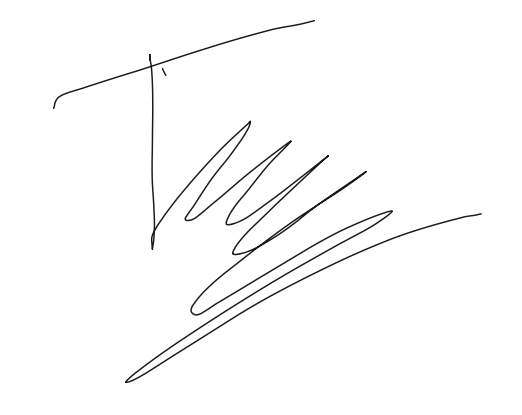
\includegraphics[width=3.8cm]{figures/common/sign.png}\\
        \vspace{0.1cm}
        \textbf{Võ Quang Thắng}
    \end{minipage}
\end{flushright}

\newpage
% --- PHẦN TIÊU ĐỀ ---
\thispagestyle{empty} % Không đánh số trang trang này (tùy chọn)
\phantomsection
\addcontentsline{toc}{chapter}{Lời cảm ơn}

\noindent
\vspace{0.2cm}
\begin{center}
    \textbf{\LARGE LỜI CẢM ƠN}
\end{center}
\vspace{1cm} % Khoảng cách từ tiêu đề xuống nội dung

% --- NỘI DUNG ---

Trong suốt thời gian học tập và nghiên cứu tại \textbf{Trường Đại học Bách Khoa - Đại học Quốc gia Thành phố Hồ Chí Minh}, em đã nhận được sự quan tâm, giảng dạy và hướng dẫn tận tình từ quý thầy cô trong khoa. Đồ án tốt nghiệp này là minh chứng cho sự nỗ lực không ngừng của em trong việc vận dụng những kiến thức đã được trang bị để giải quyết các vấn đề thực tiễn trong lĩnh vực công nghệ thông tin.

Trước tiên, em xin gửi lời cảm ơn chân thành và sâu sắc nhất đến \textbf{TS. Trương Tuấn Anh}, người thầy đã tận tâm hướng dẫn, định hướng và đồng hành cùng em trong suốt quá trình thực hiện đồ án. Thầy không chỉ truyền đạt kiến thức chuyên môn mà còn định hướng phương pháp nghiên cứu khoa học, giúp em có cái nhìn sâu sắc hơn về vấn đề đang giải quyết. Những lời khuyên, góp ý quý báu của thầy là động lực to lớn giúp em vượt qua mọi khó khăn, thử thách để hoàn thành tốt đồ án này.

Em cũng xin gửi lời cảm ơn chân thành đến \textbf{CN. Dương Huỳnh Anh Đức} đã đồng hành, hỗ trợ và đóng góp nhiều ý kiến quý báu trong quá trình thực hiện đồ án, giúp em có thêm góc nhìn thực tiễn và áp dụng hiệu quả các giải pháp kỹ thuật.

Em xin bày tỏ lòng biết ơn sâu sắc đến toàn thể quý thầy cô \textbf{Khoa Khoa học và Kỹ thuật Máy tính} đã tận tình giảng dạy, truyền đạt kiến thức và kinh nghiệm quý báu trong suốt những năm học vừa qua. Nền tảng kiến thức vững chắc mà các thầy cô đã trang bị là hành trang vô cùng quý giá để em tự tin bước vào môi trường làm việc thực tế.

Em cũng xin cảm ơn gia đình, bạn bè đã luôn bên cạnh, động viên và tạo điều kiện tốt nhất để em có thể hoàn thành tốt chương trình học tập cũng như đồ án tốt nghiệp này.

Do thời gian và kinh nghiệm có hạn, đồ án không tránh khỏi những thiếu sót. Em rất mong nhận được sự góp ý, chỉ bảo của quý thầy cô để đồ án được hoàn thiện hơn và em có thêm kinh nghiệm quý báu cho công việc sau này.

Xin chân thành cảm ơn!

% --- PHẦN KÝ TÊN ---
\vspace{0.8cm}
\begin{flushright}
    \begin{minipage}{7.2cm}
        \centering
        \textit{Tp. Hồ Chí Minh, tháng 05 năm 2026} \\
        \vspace{0.15cm}
        \textbf{Sinh viên thực hiện} \\
        \vspace{0.3cm}
        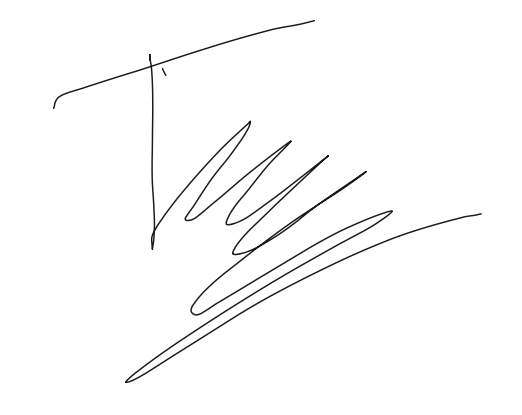
\includegraphics[width=3.8cm]{figures/common/sign.png}\\
        \vspace{0.1cm}
        \textbf{Hồ Sỹ Thắng}
    \end{minipage}
\end{flushright}

\newpage
\thispagestyle{empty}
\phantomsection
\addcontentsline{toc}{chapter}{Tóm tắt}

% --- PHẦN TIÊU ĐỀ (Mô phỏng theo mẫu ảnh bạn gửi) ---
\noindent
\vspace{0.2cm}
\begin{center}
    \textbf{\LARGE TÓM TẮT}
\end{center}
\vspace{1cm} % Khoảng cách xuống nội dung

% --- NỘI DUNG TÓM TẮT ---

Đồ án tốt nghiệp này tập trung vào việc nghiên cứu, thiết kế và xây dựng \textbf{Hệ thống Quản lý Thư viện Trực tuyến tích hợp AI}, nhằm giải quyết các hạn chế của các hệ thống thư viện truyền thống như khả năng tìm kiếm kém hiệu quả và thiếu sự cá nhân hóa. Hệ thống được phát triển với mục tiêu số hóa toàn diện quy trình vận hành thư viện, đồng thời ứng dụng trí tuệ nhân tạo để nâng cao trải nghiệm đọc và khám phá tri thức của người dùng.

Về mặt kỹ thuật, hệ thống được xây dựng dựa trên kiến trúc \textbf{Modular Monolith} với Clean Architecture + Domain-Driven Design cho từng module, đảm bảo tính bảo mật và khả năng mở rộng. Backend sử dụng \textbf{Spring Boot (Java)} để xử lý các nghiệp vụ phức tạp, kết hợp với Frontend \textbf{React + Vite} mang lại giao diện hiện đại, tốc độ build nhanh và triển khai đơn giản qua NGINX. Các chức năng chính bao gồm: quản lý tài nguyên sách, quản lý độc giả, quy trình mượn trả tự động, kiểm soát phí phạt và hệ thống báo cáo thống kê trực quan cho thủ thư.

Điểm đột phá của đồ án là việc tích hợp sâu các công nghệ AI/NLP tiên tiến. Cụ thể, hệ thống ứng dụng mô hình \textbf{Sentence-BERT (SBERT)} để thực hiện tìm kiếm ngữ nghĩa (Semantic Search), giúp xử lý các truy vấn tiếng Việt phức tạp mà không phụ thuộc vào từ khóa chính xác. Song song đó, hệ thống gợi ý sách sử dụng phương pháp lai (\textbf{Hybrid Approach}), kết hợp giữa Lọc cộng tác (Collaborative Filtering) và Lọc dựa trên nội dung (Content-Based), giúp đưa ra các đề xuất sách phù hợp nhất dựa trên lịch sử và hành vi của từng độc giả.

Kết quả của đồ án là một hệ thống phần mềm hoàn chỉnh, có giao diện thân thiện, đáp ứng đầy đủ các yêu cầu nghiệp vụ của một thư viện đại học. Hệ thống đã chứng minh được tính khả thi trong việc kết hợp giữa quản lý truyền thống và công nghệ thông minh, mang lại giá trị thực tiễn cao trong việc thúc đẩy văn hóa đọc và chuyển đổi số trong môi trường giáo dục.

\newpage
\thispagestyle{empty}
\tableofcontents
\newpage
\thispagestyle{empty}
\phantomsection
\addcontentsline{toc}{chapter}{Danh mục hình ảnh}
\listoffigures
\newpage
\thispagestyle{empty}
\phantomsection
\addcontentsline{toc}{chapter}{Danh mục bảng biểu}
\listoftables
\newpage

% --- NỘI DUNG CHÍNH (ĐÁNH SỐ Ả RẬP 1, 2, 3... VÀ CÓ TRANG X/Y) ---
\cleardoublepage
\makeatletter
\let\ps@plain\ps@fancy
\makeatother
\pagestyle{fancy}
\pagenumbering{arabic}
\setcounter{page}{1}

% % File: I.Introduction_project.tex
% Nội dung Chương 1: Giới thiệu

\chapter{Giới thiệu}
\label{chap:GioiThieu}

Chương này trình bày tổng quan về đề tài, bao gồm lý do lựa chọn, mục tiêu cần
đạt được, phạm vi nghiên cứu và phát triển, ý nghĩa khoa học--thực tiễn của dự
án, đồng thời giới thiệu cấu trúc tổng thể của báo cáo.
% ------------------------------------
\section{Động cơ của đề tài}
\label{sec:DongCo}

Trong bối cảnh chuyển đổi số giáo dục đang diễn ra mạnh mẽ, việc hiện đại hóa
các hệ thống thư viện tại trường đại học là một yêu cầu cấp thiết. Các hệ thống
thư viện hiện tại, như Koha hay OPAC-HCMUT, dù đáp ứng được nhu cầu quản lý cơ
bản nhưng vẫn còn nhiều hạn chế. Cụ thể, các hệ thống này chủ yếu dựa trên tìm
kiếm từ khóa đơn giản, chưa khai thác tốt nội dung số của tài liệu PDF, chưa có
cơ chế gợi ý dựa trên hành vi người dùng, và giao diện chưa thật sự tối ưu cho
trải nghiệm sử dụng trên nhiều thiết bị. Thêm vào đó, các nghiệp vụ như đặt
trước, nhắc hạn trả, thông báo thời gian thực, theo dõi phí phạt và thống kê xu
hướng đọc thường còn rời rạc, gây tốn nhiều thời gian cho thủ thư.

Từ thực tiễn đó, có một nhu cầu rõ rệt từ các bên liên quan:
\begin{itemize}
    \item \textbf{Sinh viên và giảng viên:} Cần một công cụ tìm kiếm tài liệu
    nhanh chóng, chính xác, hỗ trợ cả truy vấn tiếng Việt/tiếng Anh và gợi ý tài
    liệu liên quan để phục vụ học tập, nghiên cứu.
    \item \textbf{Thủ thư và nhà quản lý:} Mong muốn có một hệ thống tự động hóa
    các công việc lặp lại như quản lý ấn phẩm, bản sao, mượn--trả, đặt trước,
    phí phạt, thông báo và báo cáo thống kê.
    \item \textbf{Nhà trường:} Hướng tới việc thúc đẩy văn hóa đọc và năng lực
    số của sinh viên thông qua một nền tảng thư viện hiện đại, có khả năng mở
    rộng và tích hợp với các dịch vụ số khác.
\end{itemize}

Vì vậy, việc phát triển một \textbf{Hệ thống quản lý thư viện trực tuyến tích
hợp AI hỗ trợ tìm kiếm và gợi ý sách} là cần thiết, không chỉ để giải quyết các
hạn chế của hệ thống cũ mà còn để thử nghiệm cách kết hợp phần mềm quản lý thư
viện truyền thống với AI service xử lý nội dung tài liệu.

\section{Mục tiêu}
\label{sec:MucTieu}

Đề tài đặt ra mục tiêu tổng quát là xây dựng một hệ thống quản lý thư viện trực
tuyến thông minh, vừa đảm bảo các chức năng quản lý cốt lõi, vừa tích hợp AI/NLP
để nâng cao trải nghiệm tìm kiếm, khám phá và đọc tài liệu của người dùng.

Các mục tiêu cụ thể bao gồm:
\begin{itemize}
    \item \textbf{Xây dựng hệ thống quản lý thư viện trực tuyến:} Cung cấp các
    chức năng chính như quản lý ấn phẩm, bản sao, tác giả, nhà xuất bản, danh
    mục, tag, người dùng, mượn--trả, đặt trước, phí phạt và thông báo.
    \item \textbf{Ứng dụng AI/NLP để nâng cao trải nghiệm:}
    \begin{itemize}
        \item Phát triển công cụ tìm kiếm kết hợp lexical search và semantic
        search, hỗ trợ truy vấn tiếng Việt/tiếng Anh thông qua tag canonical và
        alias dịch.
        \item Xây dựng hệ thống gợi ý sách dựa trên hành vi người dùng, kết hợp
        content-based recommendation, collaborative filtering và fallback theo
        xu hướng.
        \item Tích hợp pipeline xử lý PDF để sinh tóm tắt nội dung, audience và
        đúng 5 tag học thuật phục vụ tìm kiếm, gợi ý và hiển thị chi tiết sách.
    \end{itemize}
    \item \textbf{Hỗ trợ công tác quản lý:} Tự động hóa thống kê, dashboard,
    nhắc hạn trả, xử lý quá hạn, hàng chờ đặt trước và thanh toán phí phạt, giúp
    thủ thư dễ dàng theo dõi vận hành thư viện.
    \item \textbf{Đảm bảo khả năng triển khai và mở rộng:} Xây dựng backend theo
    mô hình modular monolith, frontend SPA tách biệt và AI service độc lập để
    thuận tiện triển khai, kiểm thử và tách module trong tương lai.
\end{itemize}

\section{Phạm vi}
\label{sec:PhamVi}

Đề tài sẽ tập trung vào các phạm vi nghiên cứu và phát triển như sau:
\begin{itemize}
    \item \textbf{Về chức năng quản lý:} Hệ thống thực hiện các chức năng cốt
    lõi bao gồm quản lý ấn phẩm, bản sao, tác giả, nhà xuất bản, danh mục, tag,
    người dùng, vai trò, mượn--trả, đặt trước, hàng chờ, hạn trả, phí phạt,
    thanh toán, thông báo và dashboard thống kê.

    \item \textbf{Về ứng dụng AI:}
    \begin{itemize}
        \item Xây dựng hệ thống tìm kiếm kết hợp từ khóa, tag/category alias và
        vector semantic search; ưu tiên lexical search với truy vấn ngắn để giữ
        tính chính xác và dùng semantic search để mở rộng khả năng khám phá.
        \item Tích hợp hệ thống gợi ý cá nhân hóa dựa trên lịch sử xem, wishlist,
        mượn sách, đánh giá và dữ liệu vector nội dung.
        \item Phát triển mô-đun AI ETL xử lý PDF, làm sạch văn bản, chia chunk,
        sinh embedding, tóm tắt nội dung, audience và tag.
    \end{itemize}

    \item \textbf{Về nền tảng công nghệ:} Hệ thống gồm frontend React/Vite,
    backend Spring Boot modular monolith, PostgreSQL/Flyway, Kafka/WebSocket,
    S3-compatible storage, PayOS và AI service Python/FastAPI/Celery dùng
    embedding model kết hợp Gemini ở bước reduce metadata.

    \item \textbf{Về phạm vi triển khai:} Sản phẩm của đề tài là hệ thống web thật sự
    hoàn chỉnh, được kiểm chứng bằng dữ liệu và kịch bản
    nghiệp vụ phù hợp với quy mô thư viện cấp trường; một số tích hợp
    ngoài như PayOS, S3 và Gemini phụ thuộc cấu hình môi trường triển khai.
\end{itemize}

\section{Ý nghĩa}
\label{sec:YNghia}

\subsection{Ý nghĩa thực tiễn}
\label{subsec:YNghiaThucTien}
\begin{itemize}
    \item \textbf{Nâng cao trải nghiệm người dùng:} Giúp sinh viên và giảng viên
    tìm kiếm tài liệu nhanh hơn, xem được tag/tóm tắt nội dung, nhận gợi ý tài
    liệu liên quan và theo dõi trạng thái mượn--trả/đặt trước trực tuyến.
    \item \textbf{Tối ưu hóa công tác quản lý:} Giảm tải công việc thủ công cho
    thủ thư thông qua dashboard, scheduler, notification, quản lý phí phạt,
    thanh toán và các công cụ tra cứu nghiệp vụ.
    \item \textbf{Thúc đẩy chuyển đổi số:} Góp phần xây dựng mô hình thư viện số
    hiện đại, phù hợp với chủ trương chuyển đổi số trong giáo dục và phát triển
    năng lực số cho sinh viên.
\end{itemize}

\subsection{Ý nghĩa khoa học}
\label{subsec:YNghiaKhoaHoc}
\begin{itemize}
    \item \textbf{Ứng dụng AI/NLP vào bài toán thực tế:} Đề tài áp dụng xử lý
    văn bản PDF, embedding, semantic search và hệ thống gợi ý vào bài toán tìm
    kiếm tài liệu trong thư viện đại học.
    \item \textbf{Kết hợp mô hình và hệ thống:} Dự án là cầu nối giữa kỹ thuật
    AI và hệ thống phần mềm hoàn chỉnh: AI service không đứng riêng lẻ mà được
    nối với catalog, search, recommendation, notification và giao diện người
    dùng.
    \item \textbf{Đề xuất giải pháp khả thi:} Hệ thống áp dụng hướng hybrid
    search và hybrid recommendation ở mức phù hợp với dữ liệu và quy mô thư viện theo hướng tối ưu nhất giữa độ chính xác và khả năng khám phá.
\end{itemize}

\section{Cấu trúc báo cáo}
\label{sec:CauTruc}

Ngoài các phần đầu mục như Tóm tắt, Mục lục, Tài Nguyên và Mã Nguồn, Danh mục hình ảnh và bảng biểu, nội dung chính của báo cáo được cấu trúc thành 9 chương như sau:
\begin{itemize}
    \item \textbf{Chương 1 - Giới thiệu:} Trình bày tổng quan về động cơ, mục tiêu, phạm vi và ý nghĩa của đề tài, đồng thời giới thiệu cấu trúc tổng thể của báo cáo.

    \item \textbf{Chương 2 - Kiến thức và công nghệ nền tảng:} Trình bày các cơ sở lý thuyết, kiến thức chuyên ngành và các công nghệ cốt lõi được sử dụng để phát triển dự án.

    \item \textbf{Chương 3 - Công trình liên quan:} Phân tích, so sánh các nghiên cứu và hệ thống tương tự để xác định khoảng trống nghiên cứu mà đề tài giải quyết.

    \item \textbf{Chương 4 - Hệ thống đề xuất:} Mô tả tổng quan hệ thống được đề xuất, bao gồm đối tượng người dùng, yêu cầu chức năng, phi chức năng, yêu cầu dữ liệu và các luồng nghiệp vụ chính.

    \item \textbf{Chương 5 - Phân tích và Thiết kế:} Trình bày chi tiết quá trình phân tích và thiết kế hệ thống, bao gồm kiến trúc phần mềm, thiết kế cơ sở dữ liệu, thiết kế AI Service và thiết kế giao diện.

    \item \textbf{Chương 6 - Hiện thực hệ thống:} Mô tả quá trình hiện thực frontend, backend và AI service, bao gồm giao diện cho Độc giả/Thủ thư, API nghiệp vụ, pipeline xử lý dữ liệu AI và các tích hợp hạ tầng.

    \item \textbf{Chương 7 - Kiểm thử:} Trình bày chiến lược kiểm thử phân tầng cho frontend, backend và AI service, bao gồm unit/context test, controller/integration test, SQL contract test, AI metadata quality test và live Gemini artifact.

    \item \textbf{Chương 8 - Triển khai hệ thống:} Mô tả quá trình đóng gói Docker, cấu hình NGINX, CI/CD và triển khai lên môi trường VPS thực tế.

    \item \textbf{Chương 9 - Tổng kết:} Tóm tắt kết quả đạt được, nhận xét ưu điểm và hạn chế còn tồn tại của hệ thống.

    % \item \textbf{Chương 10 - Tài nguyên và Mã nguồn:} Cung cấp các đường dẫn đến mã nguồn (GitHub) và bản thiết kế giao diện (Figma) của dự án.
\end{itemize}

% \newpage
\chapter{Kiến thức và công nghệ nền tảng}

Chương này trình bày tổng quan về các kiến thức và các lĩnh vực công nghệ nền tảng được vận dụng để xây dựng "Hệ thống quản lý thư viện trực tuyến tích hợp AI hỗ trợ tìm kiếm và gợi ý sách".

\section{Các Lĩnh vực Công nghệ Chính}

Dự án được định hướng phát triển dựa trên kiến trúc phần mềm hiện đại, trong đó các thành phần chính được phân tách rõ ràng để thuận lợi cho việc bảo trì và mở rộng sau này.

\begin{itemize}
    \item \textbf{Công nghệ phía Server (Back-End):} Đây là thành phần trung tâm, chịu trách nhiệm xử lý toàn bộ logic nghiệp vụ của hệ thống, cung cấp các giao diện lập trình ứng dụng (API), quản lý dữ liệu mượn-trả, và thực hiện các tác vụ thống kê.

    \item \textbf{Công nghệ phía Client (Front-End):} Thành phần này đảm nhiệm việc xây dựng giao diện người dùng, giúp người dùng cuối (thủ thư, bạn đọc) tương tác với hệ thống một cách trực quan và thân thiện trên nền tảng web.

    \item \textbf{Hệ quản trị Cơ sở dữ liệu:} Hệ thống sử dụng một hệ quản trị cơ sở dữ liệu quan hệ để tổ chức, lưu trữ và truy xuất toàn bộ dữ liệu của thư viện, bao gồm thông tin sách, người dùng, và lịch sử giao dịch.

    \item \textbf{Trí tuệ Nhân tạo (AI) và Học máy (Machine Learning):}
    \begin{itemize}
        \item \textbf{Hệ thống gợi ý (Recommendation System):} Trọng tâm của dự án là áp dụng mô hình \textbf{Hybrid}, một phương pháp kết hợp ưu điểm của hai kỹ thuật chính:
        \begin{enumerate}
            \item \textbf{Lọc dựa trên nội dung (Content-Based Filtering):} Gợi ý tài liệu dựa trên sự tương đồng về thuộc tính và nội dung của chúng.
            \item \textbf{Lọc cộng tác (Collaborative Filtering):} Đề xuất tài liệu dựa trên hành vi và sở thích của các nhóm người dùng tương tự nhau.
        \end{enumerate}

        \item \textbf{Xử lý Ngôn ngữ Tự nhiên (NLP):} Các kỹ thuật NLP được ứng dụng để nâng cao trải nghiệm người dùng, bao gồm: phát triển công cụ \textbf{tìm kiếm ngữ nghĩa} cho tiếng Việt và tích hợp khả năng \textbf{tự động tóm tắt nội dung sách}.
    \end{itemize}
\end{itemize}

\section{Nền tảng Kiến thức Khoa học}

Việc triển khai các lĩnh vực công nghệ trên đòi hỏi các nền tảng kiến thức sau:

\begin{itemize}
    \item \textbf{Kiến trúc và Phát triển Hệ thống:}
    \begin{itemize}
        \item Hiểu biết về kiến trúc \textbf{Client-Server} và nguyên lý thiết kế \textbf{RESTful API} để đảm bảo sự giao tiếp hiệu quả giữa Front-End và Back-End.
        \item Kiến thức về thiết kế và mô hình hóa cơ sở dữ liệu quan hệ (ví dụ: ERD) để xây dựng một cấu trúc lưu trữ tối ưu.
    \end{itemize}

    \item \textbf{Khoa học Dữ liệu và Trí tuệ Nhân tạo:}
    \begin{itemize}
        \item \textbf{Nguyên lý các thuật toán gợi ý:} Nắm vững bản chất, ưu và nhược điểm của các phương pháp Content-Based, Collaborative Filtering, và cách chúng bổ trợ cho nhau trong một mô hình Hybrid.
        \item \textbf{Các kỹ thuật xử lý ngôn ngữ tự nhiên:} Có kiến thức về các phương pháp tiền xử lý văn bản, mô hình hóa ngôn ngữ (word embedding), và các thuật toán đo lường độ tương đồng ngữ nghĩa (ví dụ: \textbf{cosine similarity}).
    \end{itemize}
\end{itemize}

\textbf{Kết chương}

Nội dung chương này đã hệ thống hóa các lĩnh vực công nghệ và nền tảng kiến thức khoa học cần thiết cho dự án. Các thành phần công nghệ chính bao gồm \textbf{Back-End}, \textbf{Front-End}, \textbf{Cơ sở dữ liệu quan hệ} và các module \textbf{Trí tuệ nhân tạo}. Trọng tâm của dự án nằm ở việc áp dụng các kiến thức về \textbf{Hệ thống gợi ý Hybrid} và \textbf{Xử lý Ngôn ngữ Tự nhiên} để tạo ra một sản phẩm thông minh và khác biệt.

Các nền tảng kiến thức đã trình bày bao quát các yêu cầu lý thuyết cần thiết để triển khai dự án, từ việc xây dựng một ứng dụng web hoàn chỉnh đến tích hợp các tính năng AI nâng cao theo đúng mục tiêu đề ra.

% \chapter{Công trình liên quan}

Chương này tập trung phân tích các công trình nghiên cứu khoa học và các hệ thống phần mềm đã có liên quan đến lĩnh vực thư viện số và hệ thống gợi ý. Từ đó, chương sẽ chỉ ra những khoảng trống nghiên cứu và định vị hướng đi của đề tài.

\section{Các công trình nghiên cứu khoa học}

Qua việc tổng hợp các công trình nghiên cứu, có thể thấy các hướng tiếp cận phổ biến trong việc xây dựng hệ thống gợi ý sách cho thư viện có những đặc điểm sau:

\begin{itemize}
    \item \textbf{Ưu điểm và xu hướng chung:}
    \begin{itemize}
        \item Hầu hết các mô hình gợi ý đều theo hướng \textbf{hybrid}, kết hợp giữa Lọc dựa trên nội dung (Content-Based) và Lọc cộng tác (Collaborative Filtering) để cân bằng giữa độ cá nhân hóa và khả năng khai thác hành vi người dùng.
        \item Một số nghiên cứu cải tiến kết quả bằng cách thêm các cơ chế xếp hạng (ranking) hoặc gợi ý theo cụm người dùng (clustering), đặc biệt hiệu quả trong môi trường dữ liệu vừa và nhỏ.
        \item Việc đánh giá mô hình thường dựa trên dữ liệu thực tế từ các thư viện, giúp kiểm chứng rõ ràng hiệu quả của thuật toán.
    \end{itemize}

    \item \textbf{Hạn chế phổ biến:}
    \begin{itemize}
        \item Nhiều công trình tập trung sâu vào phần mô hình thuật toán nhưng ít chú trọng đến việc triển khai thành một hệ thống hoàn chỉnh với đầy đủ backend và frontend.
        \item Các hướng đi hiện đại như tìm kiếm ngữ nghĩa (semantic search) hay các mô hình Transformer tuy tiềm năng nhưng đòi hỏi chi phí tính toán và nguồn lực lớn, vượt quá khả năng của nhiều dự án quy mô nhỏ.
    \end{itemize}
\end{itemize}

\section{Các hệ thống và phần mềm tương tự}

Hiện nay, có nhiều hệ thống quản lý thư viện điện tử đã được triển khai rộng rãi, tiêu biểu có thể kể đến:

\begin{itemize}
    \item \textbf{Opac-HCMUT-VNU:} Là hệ thống của Đại học Quốc Gia TP.HCM, đáp ứng tốt các nghiệp vụ tra cứu và mượn-trả cơ bản. Tuy nhiên, chức năng tìm kiếm vẫn chủ yếu dựa vào từ khóa và lọc và chưa tích hợp tính năng gợi ý thông minh, tìm kiếm theo ngữ nghĩa.

    \item \textbf{Koha:} Là một phần mềm quản lý thư viện mã nguồn mở rất phổ biến, cung cấp đầy đủ chức năng quản lý và báo cáo. Mặc dù vậy, giao diện của Koha đã cũ, chưa hỗ trợ gợi ý tự động và chưa có cơ chế phân tích hành vi người dùng.

    \item \textbf{Aleph (Ex Libris):} Đây là một hệ thống thương mại quy mô lớn, tích hợp nhiều cơ sở dữ liệu học thuật. Nhược điểm chính của hệ thống này là chi phí triển khai cao và không phù hợp cho các thư viện quy mô nhỏ như cấp khoa hoặc trường đại học nhỏ.
\end{itemize}

\section{Kết chương và xác định khoảng trống nghiên cứu}

Từ việc phân tích các công trình khoa học và hệ thống thực tế, có thể nhận thấy một số \textbf{khoảng trống (gaps)} quan trọng mà đề tài này hướng đến giải quyết:

\begin{enumerate}
    \item \textbf{Khoảng trống giữa Mô hình và Thực thi:} Nhiều nghiên cứu tập trung vào việc xây dựng các mô hình gợi ý phức tạp nhưng lại bỏ qua việc triển khai chúng thành một hệ thống phần mềm hoàn chỉnh, có tính ứng dụng thực tế. Đa số các mô hình hiện nay tập trung nhiều vào thuật toán gợi ý, trong khi ít chú trọng đến việc triển khai thành hệ thống hoàn chỉnh.

    \item \textbf{Khoảng trống về Trải nghiệm Người dùng:} Các hệ thống hiện tại, kể cả mã nguồn mở như Koha, thường có giao diện cũ, chưa tối ưu cho các thiết bị hiện đại và thiếu các tính năng thông minh giúp nâng cao trải nghiệm tìm kiếm, khám phá tài liệu của người dùng.

    \item \textbf{Khoảng trống về Tính khả thi:} Các giải pháp gợi ý tiên tiến thường yêu cầu nguồn dữ liệu lớn hoặc xử lý phức tạp, vượt quá phạm vi và nguồn lực của một sinh viên thực hiện.
\end{enumerate}

\textbf{Hướng đi của dự án:} Đề tài này không đặt nặng việc phát triển một mô hình AI quá chuyên sâu. Thay vào đó, dự án tập trung vào việc \textbf{bắc cầu cho các khoảng trống trên} bằng cách:
\begin{itemize}
    \item Xây dựng một \textbf{hệ thống hoàn chỉnh} với kiến trúc frontend-backend tách biệt, dễ bảo trì và mở rộng.
    \item Ưu tiên \textbf{trải nghiệm người dùng} với giao diện hiện đại và tích hợp các tính năng gợi ý, tìm kiếm thông minh một cách liền mạch.
    \item Áp dụng một \textbf{giải pháp AI khả thi} (mô hình hybrid cơ bản) để tạo ra một sản phẩm hoạt động ổn định, có giá trị thực tiễn và phù hợp với bối cảnh của một đồ án tốt nghiệp.
\end{itemize}

% \chapter{Hệ thống đề xuất}
\label{chap:HeThongDeXuat}

\section{Mô tả hệ thống}
\label{sec:MoTaHeThong}

Hệ thống được đề xuất là một \textbf{hệ thống quản lý thư viện trực tuyến tích hợp AI hỗ trợ tìm kiếm, gợi ý và khai thác nội dung tài liệu PDF}. Mục tiêu là xây dựng một nền tảng có đủ nghiệp vụ thư viện: quản lý ấn phẩm, bản sao, người dùng, mượn--trả, đặt trước, phí phạt, thông báo và dashboard vận hành. Trên nền nghiệp vụ đó, AI được dùng ở những điểm thật sự có giá trị như làm giàu metadata từ PDF, tìm kiếm ngữ nghĩa và gợi ý tài liệu theo hành vi người dùng.

Hệ thống được thiết kế để phục vụ hai nhóm người dùng chính, mỗi nhóm có vai trò và nhu cầu riêng biệt:
\begin{itemize}
    \item \textbf{Bạn đọc (Sinh viên, Giảng viên, Nghiên cứu viên):} Là nhóm người dùng trực tiếp khai thác tài nguyên thư viện. Họ cần tìm kiếm tài liệu nhanh, xem tình trạng bản sao, đọc tóm tắt AI, thêm sách vào wishlist, đánh giá sách, gửi yêu cầu mượn, theo dõi sách đang mượn, đặt trước sách, xem phí phạt và nhận thông báo kịp thời.

    \item \textbf{Thủ thư (Người quản lý thư viện):} Là nhóm người dùng vận hành hệ thống. Thủ thư quản lý ấn phẩm, tác giả, nhà xuất bản, danh mục, tag, bản sao vật lý, upload bìa và PDF, xử lý mượn--trả tại quầy, xác nhận nhận sách, quản lý đặt trước, ghi nhận sách hư/mất, xử lý phí phạt bằng tiền mặt hoặc PayOS và theo dõi dashboard thống kê.
\end{itemize}

\section{Hướng tiếp cận thiết kế}
\label{subsec:DesignApproach}

Hệ thống Quản lý Thư viện được thiết kế theo phương pháp ``từ dưới lên''. Backend được tổ chức theo modular monolith, frontend là React SPA, còn AI service là một service riêng xử lý PDF, semantic search và recommendation.

Quá trình thiết kế được thực hiện theo các bước sau:
\begin{enumerate}
    \item Xác định các module cốt lõi của hệ thống như auth, user, catalog, circulation, recommendation và AI service.
    \item Xây dựng và kiểm thử từng module theo trách nhiệm riêng: xác thực, quản lý ấn phẩm, quản lý bản sao, giao dịch mượn--trả, thông báo, wishlist, rating, tìm kiếm và gợi ý.
    \item Tích hợp các module thành các luồng nghiệp vụ đầy đủ, ví dụ: tạo ấn phẩm, upload PDF, AI xử lý metadata, người dùng tìm kiếm, gửi yêu cầu mượn, thủ thư xác nhận và hệ thống gửi thông báo.
    \item Lặp lại quy trình này để hoàn thiện frontend, backend, AI service và các tích hợp ngoài như S3-compatible storage, Kafka/WebSocket và PayOS.
\end{enumerate}
\newpage
\section{Yêu cầu}
\label{sec:YeuCau}

\subsection{Yêu cầu chức năng}
\label{subsec:YeuCauChucNang}
Các yêu cầu chức năng của hệ thống được đặc tả chi tiết trong bảng dưới đây, phân loại theo từng nhóm chức năng và người dùng tương tác.

\begin{longtable}{|p{0.1\textwidth}|p{0.22\textwidth}|p{0.13\textwidth}|p{0.45\textwidth}|}
\caption{Bảng đặc tả yêu cầu hệ thống} \label{tab:YeuCauHeThong} \\
\hline
\textbf{ID} & \textbf{Tên yêu cầu} & \textbf{Loại} & \textbf{Mô tả chi tiết} \\
\hline
\endfirsthead
\multicolumn{4}{c}%
{{\bfseries \tablename\ \thetable{} -- tiếp theo}} \\
\hline
\textbf{ID} & \textbf{Tên yêu cầu} & \textbf{Loại} & \textbf{Mô tả chi tiết} \\
\hline
\endhead
\hline
\endfoot
%-- Yêu cầu về Dữ liệu --%
\textbf{R1} & Quản lý thực thể dữ liệu & Dữ liệu & Hệ thống phải lưu trữ và quản lý các nhóm dữ liệu cốt lõi: \textbf{ấn phẩm}, \textbf{bản sao}, \textbf{người dùng}, \textbf{giao dịch mượn--trả}, \textbf{đặt trước}, \textbf{phí phạt}, \textbf{đánh giá}, \textbf{wishlist}, \textbf{thông báo} và dữ liệu phục vụ AI. \\
\hline
\textbf{R2} & Phân biệt Ấn phẩm và Bản sao & Dữ liệu & Hệ thống phải phân biệt giữa \textbf{ấn phẩm} và \textbf{bản sao vật lý}. Mỗi bản sao có barcode riêng, trạng thái riêng, tình trạng sách và vị trí kệ để thủ thư có thể quản lý lưu thông chính xác. \\
\hline
\textbf{R3} & Thuộc tính Ấn phẩm & Dữ liệu & Mỗi ấn phẩm phải có metadata cơ bản như ISBN, tiêu đề, tác giả, nhà xuất bản, danh mục, tag, ngôn ngữ, năm xuất bản, mô tả, ảnh bìa và file PDF nếu có. Hệ thống cũng lưu summary, nhóm độc giả mục tiêu và tag do AI sinh ra sau khi xử lý tài liệu. \\
\hline
%-- Yêu cầu về Người dùng và Nghiệp vụ --%
\textbf{R4} & Quản lý vai trò người dùng & Chức năng & Hệ thống phải hỗ trợ xác thực và phân quyền theo vai trò, tối thiểu gồm \textbf{Bạn đọc} và \textbf{Thủ thư}. Bạn đọc được đăng ký, đăng nhập, quản lý hồ sơ cá nhân; thủ thư được truy cập các màn hình quản lý nghiệp vụ. \\
\hline
\textbf{R5} & Nghiệp vụ mượn--trả và phí phạt & Nghiệp vụ & Hệ thống phải hỗ trợ bạn đọc gửi yêu cầu mượn, thủ thư cho mượn trực tiếp hoặc xác nhận nhận sách, trả sách bằng barcode, ghi nhận sách hư/mất, tự tính phí quá hạn hoặc phí sự cố và xử lý thanh toán bằng tiền mặt hoặc PayOS. \\
\hline
%-- Yêu cầu về Chức năng --%
\textbf{R6} & Tìm kiếm hybrid & Chức năng & Hệ thống phải cung cấp tìm kiếm catalog theo keyword, tác giả, danh mục, tag, ngôn ngữ, năm xuất bản, chi nhánh và tình trạng bản sao; đồng thời hỗ trợ \textbf{tìm kiếm ngữ nghĩa} trên nội dung PDF thông qua AI service và pgvector. \\
\hline
\textbf{R7} & Chức năng Đặt trước & Chức năng & Bạn đọc phải có khả năng \textbf{đặt trước} sách khi cần. Hệ thống lưu hàng chờ đặt trước, cho phép bạn đọc hủy đặt trước, thủ thư tra cứu yêu cầu và xác nhận nhận sách khi bản sao sẵn sàng. \\
\hline
\textbf{R8} & Gợi ý, wishlist và đánh giá & Chức năng & Hệ thống phải hỗ trợ gợi ý sách cá nhân hóa dựa trên hành vi người dùng, có fallback khi dữ liệu còn ít; đồng thời cho phép bạn đọc thêm sách vào wishlist, đánh giá, bình luận và tương tác với review. \\
\hline
\textbf{R9} & Hệ thống thông báo tự động & Chức năng & Hệ thống phải gửi thông báo cho người dùng về các sự kiện quan trọng như yêu cầu mượn, xác nhận nhận sách, sách sắp đến hạn, sách quá hạn, phí phạt, đặt trước và phản hồi review. Thông báo được lưu trong hệ thống và đẩy realtime qua WebSocket. \\
\hline
\end{longtable}

\subsection{Yêu cầu phi chức năng}
\label{subsec:YeuCauPhiChucNang}
Hệ thống cần đảm bảo các yêu cầu phi chức năng trọng yếu sau:
\begin{itemize}
    \item \textbf{Tính khả dụng (Usability):} Giao diện người dùng phải nhất quán, trực quan và dễ học cho cả bạn đọc và thủ thư. Frontend cần hỗ trợ các luồng chính như tìm kiếm, xem chi tiết sách, đặt trước, theo dõi sách đang mượn, phí phạt, thông báo, quản lý ấn phẩm và xử lý mượn--trả trên các kích thước màn hình phổ biến.

    \item \textbf{Hiệu năng (Performance):} Các chức năng tương tác phải có thời gian phản hồi nhanh trong điều kiện tải thông thường. Các truy vấn catalog cần được phân trang; semantic search và recommendation cần giới hạn số lượng kết quả, dùng connection pool và timeout để tránh ảnh hưởng đến backend chính.

    \item \textbf{Độ tin cậy (Reliability):} Hệ thống phải hoạt động ổn định ngay cả khi một dịch vụ phụ trợ gặp lỗi. Khi AI service hoặc Gemini lỗi, hệ thống cần ghi nhận trạng thái xử lý, có fallback cho metadata/gợi ý và không làm nghẽn các nghiệp vụ chính như tra cứu, mượn--trả hoặc thanh toán.

    \item \textbf{Bảo mật (Security):} Hệ thống cần có cơ chế xác thực và phân quyền rõ ràng bằng JWT và kiểm tra vai trò ở backend. Các API quản trị chỉ dành cho thủ thư; callback từ AI service và webhook thanh toán cần được kiểm tra chữ ký hoặc cơ chế xác thực tương ứng; upload file phải đi qua đường dẫn có kiểm soát như presigned URL.

    \item \textbf{Khả năng bảo trì và mở rộng (Maintainability \& Scalability):} Mã nguồn phải được tổ chức rõ ràng theo frontend, backend và AI service. Backend theo modular monolith giúp tách ranh giới nghiệp vụ; AI service tách riêng giúp mở rộng pipeline PDF, semantic search và recommendation mà không làm phức tạp phần nghiệp vụ thư viện.
\end{itemize}

\subsection{Yêu cầu dữ liệu}
\label{subsec:YeuCauDuLieu}
Hệ thống yêu cầu và quản lý các nhóm dữ liệu chính sau:
\begin{itemize}
    \item \textbf{Dữ liệu lõi (Core Data):} Bao gồm thông tin ấn phẩm, bản sao, barcode, tác giả, nhà xuất bản, danh mục, tag, file bìa, file PDF và thông tin tài khoản người dùng.

    \item \textbf{Dữ liệu nghiệp vụ (Transactional Data):} Gồm các bản ghi yêu cầu mượn, xác nhận nhận sách, trả sách, đặt trước, phí phạt, thanh toán tiền mặt, thanh toán PayOS, trạng thái bản sao và thông báo.

    \item \textbf{Dữ liệu hành vi và AI (Behavioral/AI Data):} Gồm lịch sử tìm kiếm, lượt xem chi tiết sách, wishlist, rating, lịch sử mượn, vector embedding của chunk PDF, summary AI, audience, tag AI và trạng thái ETL. Đây là nguồn dữ liệu phục vụ semantic search và recommendation.
\end{itemize}

\textbf{Kết chương}

Chương này đã trình bày tổng quan hệ thống quản lý thư viện trực tuyến tích hợp AI. Hệ thống được định hướng như một sản phẩm hoàn chỉnh, trong đó nghiệp vụ thư viện vẫn là phần lõi, còn AI được dùng để làm giàu dữ liệu, hỗ trợ tìm kiếm ngữ nghĩa và gợi ý tài liệu.

Phần trọng tâm của chương đã đặc tả các yêu cầu cốt lõi của hệ thống, từ quản lý ấn phẩm, bản sao, người dùng, mượn--trả, đặt trước, phí phạt và thông báo cho đến các chức năng thông minh như semantic search, recommendation, wishlist và rating. Đồng thời, các \textbf{yêu cầu phi chức năng} như tính khả dụng, hiệu năng, độ tin cậy, bảo mật và khả năng bảo trì cũng được xác định theo đúng kiến trúc frontend--backend--AI service hiện tại.

Những yêu cầu này tạo thành một nền tảng vững chắc, là cơ sở để tiến hành quá trình phân tích và thiết kế chi tiết hệ thống sẽ được trình bày ở Chương 5.

% % ======= NỘI DUNG =======
\chapter{Phân tích và Thiết kế}
\label{chap:PhanTichVaThietKe}

\section{Phân tích}
\label{sec:PhanTich}

% ======= NỘI DUNG PHẦN PHÂN TÍCH USE CASE =======
\subsection{Mô hình hóa tương tác (Use-case Diagram)}
\label{subsec:BieuDoCaSuDung}

Phần phân tích use case được xây dựng theo phạm vi hệ thống đã hiện thực. Hệ
thống có các tác nhân chính gồm \textbf{Khách}, \textbf{Bạn đọc},
\textbf{Thủ thư} và \textbf{Quản trị viên}; ngoài ra còn có các hệ thống phụ
trợ như \textbf{Google OAuth}, \textbf{PayOS}, \textbf{Dịch vụ Email} và
\textbf{Gemini API}. Để giữ báo cáo trong giới hạn số trang, phần này trình bày
use case dưới dạng bảng đối chiếu thay cho các sơ đồ module chi tiết. Ranh giới
chức năng chính của hệ thống gồm nhóm xác thực/tài khoản, nhóm tra cứu tài liệu,
nhóm nghiệp vụ bạn đọc, nhóm nghiệp vụ thủ thư, nhóm quản trị và nhóm AI tự
động. Các quan hệ nghiệp vụ chính gồm: đăng ký bao gồm xác thực email; tìm kiếm
có thể mở rộng sang semantic search; mượn/đặt trước bao gồm kiểm tra điều kiện
mượn; upload PDF bao gồm xử lý AI; trả sách và báo hư/mất bao gồm tính phí và
gửi thông báo.

\begin{table}[H]
\centering
\caption{Đối chiếu nhóm Use Case với hiện thực hệ thống}
\label{tab:usecase_mapping_reality}
\begin{tabularx}{\linewidth}{|p{0.22\linewidth}|>{\raggedright\arraybackslash}X|>{\raggedright\arraybackslash}X|}
\hline
\textbf{Nhóm} & \textbf{Use case chính} & \textbf{Hiện thực tương ứng} \\
\hline
Xác thực và tài khoản & Đăng ký, xác thực email, đăng nhập thường, đăng nhập Google, refresh token, quên/đặt lại mật khẩu, hồ sơ, avatar, đổi mật khẩu, thông báo & Auth/User modules, OAuth2 Google, JWT/refresh token, email verification/reset password, profile API và notification API. \\
\hline
Tra cứu và khám phá tài liệu & Trang chủ, tìm kiếm catalog, semantic search, lọc danh mục/tag, chi tiết tài liệu, bản sao, đánh giá, sách tương tự, thống kê công khai & Public pages và catalog/recommendation API: \texttt{/api/v1/publications/search}, \texttt{/api/v1/ai/semantic-search}, \texttt{/api/v1/publications/\{id\}}, \texttt{/items}, \texttt{/ratings}, \texttt{/similar}. \\
\hline
Chức năng bạn đọc & Mượn, đặt trước, hủy đặt trước, theo dõi sách đang mượn, lịch sử mượn trả, phí phạt, PayOS, wishlist, rating, gợi ý cá nhân hóa & Reader pages, circulation/reservation/fine APIs, PayOS payment, wishlist/rating APIs và recommendation API. \\
\hline
Chức năng thủ thư & Quản lý ấn phẩm, bản sao, upload bìa/PDF, AI ETL, xử lý yêu cầu mượn, mượn trực tiếp, trả sách, báo hư/mất, ghi chú giao dịch, thu tiền mặt & Librarian pages, catalog/item APIs, presigned upload, backend AI gateway, circulation transaction APIs, fine cash payment và notification/email events. \\
\hline
Chức năng quản trị & Quản lý thủ thư, quản lý người dùng, khóa/mở khóa, xác minh tài khoản, chính sách mượn trả, nhật ký hệ thống & Admin pages và admin APIs: librarian/user management, circulation policy, audit log và account verification. \\
\hline
AI và xử lý tự động & Semantic search, recommendation, sách tương tự, xử lý PDF, trích xuất text, embedding, sinh summary/tag/audience, ghi nhận tương tác, realtime/email notification & AI service FastAPI/Celery, RabbitMQ, Gemini API, PostgreSQL pgvector, interaction tracking, Kafka/email/WebSocket notification. \\
\hline
\end{tabularx}
\end{table}

\subsection{Mô hình hóa luồng xử lý (Activity Diagram)}
\label{subsec:activity-diagram}

Activity Diagram được dùng để mô tả các luồng xử lý chính sau khi đã xác định
use case. Phần mô hình hóa tập trung vào các nghiệp vụ có nhiều bước và có tương tác giữa
người dùng, giao diện, backend và dịch vụ phụ trợ: xác thực, tra cứu, mượn--trả,
quản lý sách, đánh giá, xử lý hàng chờ và gợi ý sách.

\begin{figure}[H]
    \centering
    \begin{subfigure}[t]{0.48\linewidth}
        \centering
        \includegraphics[width=\linewidth, height=0.38\textheight, keepaspectratio]{figures/ch05/activity/sign_up.png}
        \caption{Đăng ký tài khoản}
    \end{subfigure}
    \hfill
    \begin{subfigure}[t]{0.48\linewidth}
        \centering
        \includegraphics[width=\linewidth, height=0.38\textheight, keepaspectratio]{figures/ch05/activity/login.png}
        \caption{Đăng nhập}
    \end{subfigure}
    \caption{Activity Diagram cho xác thực người dùng}
    \label{fig:activity_auth}
\end{figure}

\begin{figure}[H]
    \centering
    \begin{subfigure}[t]{0.48\linewidth}
        \centering
        \includegraphics[width=\linewidth, height=0.38\textheight, keepaspectratio]{figures/ch05/activity/search_book.png}
        \caption{Tìm kiếm sách}
    \end{subfigure}
    \hfill
    \begin{subfigure}[t]{0.48\linewidth}
        \centering
        \includegraphics[width=\linewidth, height=0.38\textheight, keepaspectratio]{figures/ch05/activity/suggest_book.png}
        \caption{Gợi ý sách}
    \end{subfigure}
    \caption{Activity Diagram cho tra cứu và gợi ý tài liệu}
    \label{fig:activity_search_suggest}
\end{figure}

\begin{figure}[H]
    \centering
    \begin{subfigure}[t]{0.48\linewidth}
        \centering
        \includegraphics[width=\linewidth, height=0.38\textheight, keepaspectratio]{figures/ch05/activity/borrow_book.png}
        \caption{Mượn sách}
    \end{subfigure}
    \hfill
    \begin{subfigure}[t]{0.48\linewidth}
        \centering
        \includegraphics[width=\linewidth, height=0.38\textheight, keepaspectratio]{figures/ch05/activity/return_book.png}
        \caption{Trả sách}
    \end{subfigure}
    \caption{Activity Diagram cho nghiệp vụ mượn--trả}
    \label{fig:activity_borrow_return}
\end{figure}

\begin{figure}[H]
    \centering
    \begin{subfigure}[t]{0.48\linewidth}
        \centering
        \includegraphics[width=\linewidth, height=0.38\textheight, keepaspectratio]{figures/ch05/activity/process_queue.png}
        \caption{Xử lý hàng chờ đặt trước}
    \end{subfigure}
    \hfill
    \begin{subfigure}[t]{0.48\linewidth}
        \centering
        \includegraphics[width=\linewidth, height=0.38\textheight, keepaspectratio]{figures/ch05/activity/review_and_comment.png}
        \caption{Đánh giá và bình luận}
    \end{subfigure}
    \caption{Activity Diagram cho đặt trước và tương tác sau mượn}
    \label{fig:activity_queue_review}
\end{figure}

\begin{figure}[H]
    \centering
    \includegraphics[width=0.72\linewidth, height=0.55\textheight, keepaspectratio]{figures/ch05/activity/add_book.png}
    \caption{Activity Diagram cho nghiệp vụ thêm sách}
    \label{fig:activity_add_book}
\end{figure}
\subsection{Mô hình lớp (Class diagram)}
\label{subsec:ClassDiagram}

Class diagram trong Hình~\ref{fig:class_diagram_lms} mô tả các lớp domain
chính của hệ thống theo hai cụm lớn: Core Domain và Extended Services. Trong đó,
Core Domain bao gồm User, Catalog và Circulation; Extended Services bao gồm
Reader Data, AI và Support. Sơ đồ tập trung vào entity, thuộc tính nghiệp vụ
quan trọng và quan hệ giữa các lớp, giúp liên kết phần
phân tích use case với thiết kế dữ liệu và cấu trúc backend.

\begin{figure}[H]
 \centering
 \includegraphics[width=\linewidth,height=0.9\textheight,keepaspectratio]{figures/ch05/class/classdiagram.png}
 \caption{Class diagram tổng quát của hệ thống}
 \label{fig:class_diagram_lms}
\end{figure}
\subsection{Công nghệ được sử dụng}
\label{subsec:technologies-used}
\begin{table}[H]
\centering
\small
\renewcommand{\arraystretch}{1.18}
\setlength{\tabcolsep}{4pt}
\begin{tabularx}{\linewidth}{|p{2.2cm}|p{4.1cm}|X|}
\hline
\textbf{Phần} & \textbf{Công nghệ} & \textbf{Vai trò trong hệ thống} \\
\hline
\textbf{Frontend} & React, TypeScript, Vite & Xây dựng SPA, chia trang theo vai trò và phát triển giao diện có kiểm soát kiểu dữ liệu. \\
\hline
\textbf{Frontend} & Tailwind CSS, lucide-react, sonner & Thiết kế giao diện, icon, toast notification và trạng thái tương tác. \\
\hline
\textbf{Frontend} & React Router/HashRouter & Điều hướng public/user/librarian/admin page và bảo vệ route theo vai trò. \\
\hline
\textbf{Frontend} & Context API & Quản lý trạng thái dùng chung như đăng nhập, ngôn ngữ, theme, notification và upload. \\
\hline
\textbf{Frontend} & Axios, STOMP/SockJS & Gọi REST API, gắn JWT/refresh token và nhận thông báo realtime qua WebSocket. \\
\hline
\textbf{Frontend} & Jest, Testing Library, Nginx & Kiểm thử frontend và phục vụ bản build static trong container production. \\
\hline
\textbf{Backend} & Java 21, Spring Boot & Hiện thực API nghiệp vụ theo mô hình modular monolith. \\
\hline
\textbf{Backend} & Spring Security, JWT, OAuth2 & Xác thực, phân quyền, refresh token và đăng nhập Google. \\
\hline
\textbf{Backend} & Spring Data JPA, Flyway & Truy cập dữ liệu, quản lý entity và migration cơ sở dữ liệu. \\
\hline
\textbf{Backend} & PostgreSQL, pgvector & Lưu dữ liệu nghiệp vụ, metadata AI và vector phục vụ semantic search. \\
\hline
\textbf{Backend} & Kafka, WebSocket & Phát sự kiện và đẩy thông báo realtime đến người dùng. \\
\hline
\textbf{Backend} & RabbitMQ, S3-compatible Storage & Gửi job xử lý AI và lưu trữ ảnh bìa/PDF thông qua presigned URL. \\
\hline
\textbf{Backend} & PayOS, Gmail SMTP, OpenAPI/Swagger & Thanh toán phí phạt, gửi email và tài liệu hóa API. \\
\hline
\textbf{Backend} & JUnit, Mockito, Testcontainers & Kiểm thử unit/controller và integration với PostgreSQL thật. \\
\hline
\textbf{Backend} & Docker, Docker Compose & Đóng gói backend và triển khai cùng các dịch vụ phụ trợ. \\
\hline
\textbf{AI Service} & Python, FastAPI & Xây dựng API cho semantic search, similar books, recommendation và health check. \\
\hline
\textbf{AI Service} & Celery, RabbitMQ & Xử lý job AI bất đồng bộ sau khi thủ thư upload PDF. \\
\hline
\textbf{AI Service} & PyMuPDF & Trích xuất văn bản từ PDF trước khi làm sạch và chia chunk. \\
\hline
\textbf{AI Service} & SentenceTransformer/SBERT & Sinh embedding tiếng Việt cho chunk tài liệu và truy vấn tìm kiếm. \\
\hline
\textbf{AI Service} & Gemini API & Sinh summary, audience và tag học thuật ở bước metadata enrichment. \\
\hline
\textbf{AI Service} & PostgreSQL, pgvector & Lưu vector, ETL run, search log và dữ liệu phục vụ truy vấn nearest-neighbor. \\
\hline
\textbf{AI Service} & ALS implicit feedback, content-based, trending fallback & Tạo gợi ý sách cá nhân hóa và fallback khi dữ liệu tương tác còn ít. \\
\hline
\textbf{AI Service} & pytest, Docker & Kiểm thử AI Service và đóng gói FastAPI/Celery Worker để chạy tách biệt trong production. \\
\hline
\end{tabularx}
\caption{Công nghệ được sử dụng trong hệ thống}
\label{tab:technologies_used}
\end{table}
Các công nghệ trong hệ thống được chọn theo đúng phạm vi hiện thực: frontend
phục vụ trải nghiệm người dùng, backend xử lý nghiệp vụ thư viện và AI Service
xử lý các tác vụ tìm kiếm/gợi ý thông minh. Bảng dưới đây gom các công nghệ
chính đã sử dụng trong toàn hệ thống.

\section{Ứng dụng AI vào hệ thống}
% =========================================================================================
Trong hệ thống LMS, AI không được đặt vào như một chức năng phụ để ``làm đẹp'' sản phẩm. AI được thiết kế như một \textbf{lớp năng lực hỗ trợ khám phá tri thức}: đọc nội dung PDF, hiểu ý định tìm kiếm của bạn đọc và đề xuất tài liệu phù hợp với hành vi sử dụng thật.

Điểm quan trọng nhất trong thiết kế là \textbf{AI không thay thế nghiệp vụ thư viện}. Các nghiệp vụ như mượn--trả, đặt trước, quản lý bản sao, phí phạt, thanh toán và phân quyền vẫn do backend Spring Boot kiểm soát. AI Service chỉ xử lý các bài toán phù hợp với ML/NLP, sau đó trả về \textbf{metadata bổ trợ}, \textbf{danh sách \texttt{publication\_id}} hoặc \textbf{chiến lược gợi ý}; backend luôn là nơi lấy dữ liệu cuối cùng trước khi trả về frontend.

\begin{itemize}
    \item \textbf{Module 1 -- Xử lý PDF file:} biến file PDF do thủ thư upload thành dữ liệu có thể tìm kiếm và gợi ý.
    \item \textbf{Module 2 -- Hỗ trợ tìm kiếm ngữ nghĩa:} giúp bạn đọc tìm theo ý định, không chỉ theo từ khóa chính xác.
    \item \textbf{Module 3 -- Gợi ý cá nhân hoá:} kết hợp nội dung sách, hành vi người dùng và fallback nghiệp vụ để đề xuất sách có thể mượn.
\end{itemize}

Dự án chọn mô hình \textbf{AI Satellite Service}: backend Java giữ nghiệp vụ và giao dịch; AI Service Python/FastAPI xử lý workload nặng như đọc PDF, sinh embedding, truy vấn pgvector và recommendation. Cách tách này giúp hệ thống vừa \textbf{giữ lõi nghiệp vụ ổn định}, vừa \textbf{tận dụng hệ sinh thái AI của Python}.

Về mặt giá trị sử dụng, AI giải quyết ba điểm yếu thường gặp của hệ thống thư
viện truyền thống. Thứ nhất, nhiều tài liệu chỉ được mô tả bằng tiêu đề và vài
trường metadata, trong khi nội dung thật nằm sâu trong PDF; pipeline AI giúp
biến phần nội dung đó thành dữ liệu có thể tìm kiếm. Thứ hai, người đọc thường
tìm bằng nhu cầu học tập thay vì từ khóa chính xác; semantic search giúp hệ
thống hiểu gần đúng ý định truy vấn. Thứ ba, danh mục thư viện càng lớn thì
người dùng càng khó chọn sách phù hợp; recommendation dùng hành vi đọc, wishlist,
mượn và rating để rút ngắn quá trình khám phá tài liệu.

\begin{table}[H]
\centering
\small
\renewcommand{\arraystretch}{1.16}
\setlength{\tabcolsep}{5pt}
\begin{tabularx}{\linewidth}{|>{\bfseries}p{0.24\linewidth}|>{\raggedright\arraybackslash}X|>{\raggedright\arraybackslash}X|}
\hline
\textbf{Vấn đề} & \textbf{Thiết kế AI trong hệ thống} & \textbf{Giá trị đạt được} \\
\hline
Tài liệu PDF khó khai thác & Trích xuất nội dung, làm sạch, chia chunk, sinh embedding và summary/tag. & Sách không chỉ được tìm bằng metadata nhập tay mà còn bằng nội dung thật. \\
\hline
Truy vấn người dùng không chính xác & Mã hóa query thành vector và so khớp với vector chunk trong pgvector. & Người đọc có thể tìm theo ý định như ``sách nhập môn dễ hiểu'' hoặc ``tài liệu về chuẩn hóa dữ liệu''. \\
\hline
Khó chọn sách phù hợp & Kết hợp content-based, ALS implicit feedback và trending fallback. & Gợi ý vẫn hoạt động khi người dùng mới, sách mới hoặc dữ liệu tương tác còn ít. \\
\hline
AI có thể lỗi hoặc hết quota & Backend giữ nghiệp vụ chính; AI có timeout, retry, fallback và trạng thái xử lý rõ ràng. & Lỗi AI không làm hỏng catalog, mượn--trả, đặt trước hoặc thanh toán. \\
\hline
\end{tabularx}
\caption{Giá trị thiết kế của lớp AI trong hệ thống}
\label{tab:ai_design_value}
\end{table}

Một nguyên tắc quan trọng là \textbf{AI chỉ làm giàu dữ liệu, không tự quyết định
nghiệp vụ}. Ví dụ, semantic search có thể trả danh sách \texttt{publication\_id}
phù hợp, nhưng backend vẫn kiểm tra sách còn bản sao hay không, người dùng có
quyền mượn hay không và dữ liệu nào được phép hiển thị. Tương tự, recommendation
chỉ đề xuất ứng viên; trạng thái cuối cùng của sách, phí phạt, đặt trước và phân
quyền vẫn nằm trong các module nghiệp vụ của backend. Nhờ vậy, hệ thống tận dụng
được AI nhưng không đánh đổi tính nhất quán dữ liệu.

\begin{figure}[H]
\centering
\begin{tikzpicture}[
    % Sử dụng positioning giúp quản lý khoảng cách các khối linh hoạt và rộng rãi hơn
    node distance=1.5cm and 2.5cm,
    every node/.style={font=\small\sffamily},
    box/.style={rectangle, draw=blue!65!black, fill=blue!5, thick, rounded corners=3pt, minimum width=3.5cm, minimum height=1.2cm, align=center},
    ai/.style={rectangle, draw=green!55!black, fill=green!6, thick, rounded corners=3pt, minimum width=3.5cm, minimum height=1.2cm, align=center},
    db/.style={cylinder, draw=orange!80!black, fill=orange!7, shape border rotate=90, aspect=0.22, minimum width=2.5cm, minimum height=1.5cm, align=center},
    arrow/.style={thick, ->, >=stealth},
    label text/.style={font=\small, midway}
]
    % --- Định nghĩa các khối hệ thống (Nodes) ---
    \node[box] (fe) {Frontend\\React/Vite};
    \node[box, right=of fe] (be) {Backend\\Spring Boot};
    \node[ai, right=of be] (ai) {AI Service\\FastAPI};

    \node[db, below=of be] (pg) {PostgreSQL\\Catalog};
    \node[db, below=of ai] (vec) {pgvector\\AI schema};

    % --- Định nghĩa đường nối luồng dữ liệu (Arrows) ---
    \draw[arrow] (fe) -- node[label text, above] {REST API} (be);
    \draw[arrow] (be) -- node[label text, above] {AI Gateway} (ai);
    \draw[arrow] (be) -- node[label text, left] {nghiệp vụ} (pg);
    \draw[arrow] (ai) -- node[label text, right] {vectors / ETL / cache} (vec);
    \draw[arrow] (vec) -- node[label text, above] {publication ids} (pg);
\end{tikzpicture}
\caption{Trách nhiệm giữa frontend, backend và AI service}
\label{fig:ai_integration_boundary}
\end{figure}

\begin{table}[H]
\centering
\small
\renewcommand{\arraystretch}{1.18}
\setlength{\tabcolsep}{5pt}
\begin{tabularx}{\linewidth}{|>{\bfseries}p{0.23\linewidth}|>{\raggedright\arraybackslash}X|>{\raggedright\arraybackslash}X|}
\hline
\textbf{Thành phần} & \textbf{Trách nhiệm chính} & \textbf{Điểm nhấn thiết kế} \\
\hline
Frontend & Upload tài liệu, gửi truy vấn, hiển thị trạng thái AI và kết quả đã chuẩn hóa. & \textbf{Không gọi trực tiếp model AI}; mọi request đi qua backend. \\
\hline
Backend & Xác thực, phân quyền, lưu catalog, quản lý bản sao/giao dịch và lấy metadata cuối cùng. & \textbf{Là nguồn sự thật nghiệp vụ}; AI không được quyết định trạng thái mượn--trả. \\
\hline
AI Service & Xử lý PDF, sinh embedding, tìm kiếm ngữ nghĩa, tạo metadata AI và recommendation. & \textbf{Chỉ trả kết quả suy luận}; backend quyết định dữ liệu hiển thị cuối cùng. \\
\hline
\end{tabularx}
\caption{Ranh giới trách nhiệm khi tích hợp AI}
\label{tab:ai_responsibility_boundary}
\end{table}

\subsection{Cơ sở thiết kế dữ liệu AI}

Trước khi hiện thực, thiết kế xác định rõ AI cần ba nhóm dữ liệu đầu vào. Cách
thiết kế này giúp tránh tình trạng ``có model trước rồi mới tìm dữ liệu'', đồng
thời bảo đảm mỗi thuật toán đều có nguồn tín hiệu khả thi trong hệ thống thư
viện.

\begin{table}[H]
\centering
\small
\renewcommand{\arraystretch}{1.18}
\setlength{\tabcolsep}{4pt}
\begin{tabularx}{\linewidth}{|>{\bfseries}p{0.2\linewidth}|>{\raggedright\arraybackslash}X|>{\raggedright\arraybackslash}X|}
\hline
\textbf{Nhóm dữ liệu} & \textbf{Nguồn trong hệ thống} & \textbf{Dùng cho bài toán AI} \\
\hline
Nội dung tài liệu & PDF, tiêu đề, phụ đề, mô tả, mục lục, tác giả, danh mục, tag. & Embedding, semantic search, sách tương tự, content-based recommendation. \\
\hline
Hành vi người dùng & Lượt xem, wishlist, mượn sách, rating, lịch sử tìm kiếm. & Collaborative filtering, ALS implicit feedback, trending fallback. \\
\hline
Trạng thái nghiệp vụ & Sách còn bản sao hay không, chi nhánh, trạng thái bản sao, quyền truy cập. & Lọc kết quả cuối cùng để gợi ý/tìm kiếm có giá trị sử dụng thật. \\
\hline
\end{tabularx}
\caption{Nguồn dữ liệu dùng cho thiết kế AI}
\label{tab:ai_data_sources_design}
\end{table}

Về mặt lưu trữ, thiết kế chọn hướng \textbf{vector theo chunk} thay vì một vector
duy nhất cho cả sách. Một sách có thể bao gồm nhiều chủ đề; nếu chỉ dùng một
vector trung bình cho toàn bộ tài liệu, các chương nhỏ nhưng quan trọng dễ bị
loãng. Vì vậy, mỗi chunk có một embedding riêng và liên kết về
\texttt{publication\_id}.

\begin{lstlisting}[language=SQL, caption={Thiết kế bảng vector phục vụ semantic search}, label={lst:ai_vector_schema_design}]
CREATE TABLE ai_engine.publication_vectors (
    id BIGSERIAL PRIMARY KEY,
    publication_id BIGINT NOT NULL,
    chunk_index INT NOT NULL,
    chunk_text TEXT NOT NULL,
    embedding VECTOR(768) NOT NULL,
    created_at TIMESTAMP DEFAULT NOW()
);

CREATE INDEX idx_publication_vectors_embedding
ON ai_engine.publication_vectors
USING hnsw (embedding vector_cosine_ops);
\end{lstlisting}

\FloatBarrier

\subsection{Module 1: Xử lý PDF file}

\textbf{Mục tiêu của module này} là biến một file PDF thô thành dữ liệu có giá trị cho hệ thống: \textbf{summary}, \textbf{audience}, \textbf{tag}, \textbf{vector embedding} và \textbf{trạng thái xử lý AI}. Đây là module nền tảng: nếu PDF không được xử lý tốt, semantic search và recommendation phía sau sẽ không có đủ dữ liệu để hoạt động.

Luồng xử lý được thiết kế theo hướng \textbf{không chặn thao tác của thủ thư}. Thủ thư chỉ cần upload tài liệu; backend lưu URL tài liệu và kích hoạt AI xử lý ở phía sau.

Phần xử lý PDF được chia thành hai nhánh rõ ràng: \textbf{ETL cục bộ} và
\textbf{LLM reduce}. ETL cục bộ chịu trách nhiệm đọc file, làm sạch văn bản,
chia chunk và sinh embedding. LLM chỉ được dùng ở bước tổng hợp metadata cuối
cùng, không tham gia vào mọi truy vấn tìm kiếm. Cách thiết kế này giúp hệ thống
giảm chi phí gọi LLM, tránh phụ thuộc quá mạnh vào quota Gemini và vẫn giữ được
dữ liệu vector ổn định để phục vụ semantic search.

Với một tài liệu sau khi trích xuất được chuỗi văn bản $D$, hệ thống chia tài
liệu thành các chunk $c_i$ theo cửa sổ trượt:

\[
C = \{c_1, c_2, ..., c_n\}, \quad |c_i| \leq L,\quad overlap(c_i,c_{i+1}) = O
\]

Trong đó $L$ là kích thước chunk tối đa và $O$ là phần chồng lắp giữa hai chunk
liền kề. Overlap giúp giảm rủi ro một ý quan trọng bị cắt giữa hai đoạn. Mỗi
chunk được mã hóa thành vector:

\[
v_i = Encoder(c_i), \quad v_i \in \mathbb{R}^{768}
\]

Các vector này được lưu trong PostgreSQL/pgvector cùng với \texttt{publication\_id}
và \texttt{chunk\_index}. Nhờ vậy, hệ thống có thể truy vấn theo nội dung thật
của sách thay vì chỉ tìm trên tiêu đề, tác giả hoặc mô tả ngắn.

\begin{figure}[H]
\centering
\resizebox{\linewidth}{!}{%
\begin{tikzpicture}[
    every node/.style={font=\small},
    flowstep/.style={rectangle, draw=blue!70!black, fill=blue!5, thick, rounded corners, minimum width=3.05cm, minimum height=1.0cm, align=center},
    store/.style={cylinder, draw=orange!80!black, fill=orange!8, shape border rotate=90, aspect=0.25, minimum width=2.3cm, minimum height=1.35cm, align=center},
    resultnode/.style={rectangle, draw=green!55!black, fill=green!6, thick, rounded corners, minimum width=3.2cm, minimum height=1.0cm, align=center},
    arrow/.style={thick, ->, >=stealth}
]
    \node[flowstep] (fe) at (0,0) {1. Thủ thư\\chọn PDF};
    \node[flowstep] (url) at (3.8,0) {2. Backend cấp\\upload URL};
    \node[store] (s3) at (7.2,0) {Object\\Storage};
    \node[flowstep] (save) at (10.8,0) {3. Lưu\\\texttt{file\_url}};
    \node[resultnode] (ai) at (10.8,-2.0) {4. Gọi AI\\process PDF};
    \node[resultnode] (etl) at (7.2,-2.0) {5. Clean\\chunk\\embed};
    \node[resultnode] (meta) at (3.8,-2.0) {6. Gemini\\reduce metadata};
    \node[store] (db) at (0,-2.0) {DB\\AI outputs};

    \draw[arrow] (fe) -- (url);
    \draw[arrow] (url) -- (s3);
    \draw[arrow] (s3) -- (save);
    \draw[arrow] (save) -- (ai);
    \draw[arrow] (ai) -- (etl);
    \draw[arrow] (etl) -- (meta);
    \draw[arrow] (meta) -- (db);
\end{tikzpicture}
}
\caption{Module 1 -- Luồng xử lý PDF file sau khi thủ thư upload}
\label{fig:ai_pdf_processing_flow}
\end{figure}

\begin{table}[H]
\centering
\small
\renewcommand{\arraystretch}{1.15}
\setlength{\tabcolsep}{4pt}
\begin{tabularx}{\linewidth}{|>{\bfseries}p{0.23\linewidth}|>{\raggedright\arraybackslash}X|>{\raggedright\arraybackslash}X|}
\hline
\textbf{Thành phần} & \textbf{Cách sử dụng trong hệ thống} & \textbf{Lý do thiết kế} \\
\hline
PyMuPDF & Đọc PDF, trích xuất text theo trang, bỏ qua ảnh bìa hoặc phần không có text. & Nhẹ, chạy được trong AI container và phù hợp với tài liệu thư viện dạng PDF. \\
\hline
Text cleaning & Chuẩn hóa khoảng trắng, bỏ số trang/header/footer lặp, giới hạn đoạn quá ngắn. & Giảm nhiễu trước khi sinh embedding và trước khi gửi dữ liệu cho LLM. \\
\hline
Sliding window chunking & Chia văn bản thành các chunk có overlap để giữ ngữ cảnh liên tục. & Tăng khả năng tìm trúng đoạn liên quan khi truy vấn theo ý nghĩa. \\
\hline
SentenceTransformer/SBERT & Sinh embedding 768 chiều cho từng chunk và query. & Phù hợp mô hình bi-encoder, vector được tính trước nên tìm kiếm nhanh. \\
\hline
Gemini reduce & Nhận một phần nội dung đại diện, sinh summary, audience và tag theo JSON. & LLM chỉ dùng để làm giàu metadata, không nằm trên đường tìm kiếm chính. \\
\hline
Fallback metadata & Nếu Gemini lỗi/quota hết, dùng title, author, category và tag sẵn có để tạo metadata tối thiểu. & AI lỗi không làm hỏng catalog và không chặn thủ thư tiếp tục vận hành. \\
\hline
\end{tabularx}
\caption{Các thành phần kỹ thuật trong Module 1}
\label{tab:ai_pdf_components}
\end{table}

\begin{lstlisting}[language={}, caption={Prompt rút gọn metadata bằng LLM}, label={lst:ai_llm_prompt}]
You are an assistant for a Vietnamese library management system.
Read the book content excerpts and return ONLY valid JSON.

Required JSON schema:
{
  "summary": "3-5 concise Vietnamese sentences",
  "audience": "target readers, e.g. beginner/intermediate/advanced",
  "tags_vi": ["3-8 Vietnamese subject tags"],
  "tags_en": ["English aliases for search expansion"]
}

Rules:
- Do not invent authors, publisher, ISBN or facts not present in the input.
- Prefer academic/library subject terms.
- Keep tags short, reusable and searchable.
- If the content is insufficient, infer only from title/category.
\end{lstlisting}

Prompt trên được thiết kế có ràng buộc đầu ra JSON để backend và AI Service dễ
parse kết quả. Các trường \texttt{tags\_vi} và \texttt{tags\_en} được giữ song
song nhằm hỗ trợ tìm kiếm song ngữ: người dùng có thể nhập từ khóa tiếng Việt
hoặc tiếng Anh nhưng vẫn tìm được cùng một nhóm tài liệu.

\begin{table}[H]
\centering
\small
\renewcommand{\arraystretch}{1.15}
\setlength{\tabcolsep}{4pt}
\begin{tabularx}{\linewidth}{|>{\bfseries}p{0.22\linewidth}|>{\raggedright\arraybackslash}X|>{\raggedright\arraybackslash}X|}
\hline
\textbf{Giai đoạn} & \textbf{Thiết kế} & \textbf{Điểm nhấn báo cáo} \\
\hline
Upload và lưu file & Frontend xin \textbf{presigned upload URL}; file PDF được đẩy lên object storage; backend lưu lại \texttt{file\_url}/\texttt{s3Key} cho publication. & \textbf{File được lưu trước, AI xử lý sau}; thao tác tạo/cập nhật sách không bị khóa bởi pipeline AI. \\
\hline
ETL nội dung & AI Service dùng \textbf{PyMuPDF} để trích xuất text, làm sạch header/footer/số trang, sau đó chia chunk bằng sliding window. & \textbf{Index nội dung thật của PDF}, không chỉ index tiêu đề hay mô tả thủ công. \\
\hline
Embedding và metadata & Chunk được vector hóa và lưu vào \texttt{ai\_engine.publication\_vectors}; Gemini chỉ được gọi ở bước reduce để tạo summary, audience và tag. & \textbf{Không gọi LLM trong mỗi lần tìm kiếm}; giảm độ trễ, giảm quota và tăng độ ổn định. \\
\hline
Theo dõi trạng thái & Kết quả xử lý được lưu với trạng thái \texttt{RUNNING}, \texttt{SUCCESS}, \texttt{FAILED}; nếu lỗi, catalog vẫn giữ ấn phẩm. & \textbf{AI lỗi không làm hỏng nghiệp vụ thư viện}. \\
\hline
\end{tabularx}
\caption{Thiết kế Module 1 -- Xử lý PDF file}
\label{tab:ai_module_pdf}
\end{table}

\subsection{Module 2: Hỗ trợ tìm kiếm ngữ nghĩa (Semantic Search)}

\textbf{Mục tiêu của module này} là giúp bạn đọc tìm được tài liệu theo \textbf{ý định học tập}, không bị phụ thuộc hoàn toàn vào việc nhớ đúng tên sách, tác giả hoặc tag. Ví dụ, truy vấn ``sách nhập môn cơ sở dữ liệu dễ hiểu'' vẫn có thể tìm đến các tài liệu liên quan, dù cụm từ đó không xuất hiện nguyên văn trong tiêu đề.

Về mặt thiết kế, hệ thống dùng hướng \textbf{Bi-Encoder} của Sentence-BERT \cite{Reimers2019SentenceBERT}: vector của chunk PDF được tính trước trong Module 1, còn vector của query được tính tại thời điểm tìm kiếm. Việc so khớp vector được thực hiện bằng \textbf{PostgreSQL + pgvector} \cite{pgvector_docs}.

Khi người dùng nhập truy vấn $q$, AI Service sinh vector truy vấn:

\[
v_q = Encoder(q)
\]

Độ phù hợp giữa truy vấn và một chunk được tính bằng cosine similarity:

\[
sim(q,c_i) = \frac{v_q \cdot v_i}{\|v_q\| \|v_i\|}
\]

Vì mỗi sách có nhiều chunk, điểm semantic của một ấn phẩm không lấy trung bình
toàn bộ chunk mà lấy điểm tốt nhất trong các chunk liên quan:

\[
S_{semantic}(q,p) = \max_{c_i \in p} sim(q,c_i)
\]

Điểm cuối cùng được chuẩn hóa và kết hợp thêm tín hiệu keyword để tránh trường
hợp truy vấn rất rõ ràng như tên sách hoặc tên tác giả bị semantic search làm
lệch kết quả:

\[
S_{search}(q,p) =
0.70 \times S_{semantic}(q,p)
+ 0.20 \times S_{keyword}(q,p)
+ 0.10 \times S_{freshness}(p)
\]

Trong đó $S_{keyword}$ đến từ tiêu đề, tác giả, category, tag; còn
$S_{freshness}$ là điểm ưu tiên nhẹ cho tài liệu mới hoặc vừa được cập nhật.
Trọng số này được chọn theo hướng ưu tiên ý nghĩa nội dung nhưng vẫn giữ kết quả
ổn định với các truy vấn định danh.

\begin{figure}[H]
\centering
\resizebox{\linewidth}{!}{%
\begin{tikzpicture}[
    every node/.style={font=\small},
    box/.style={rectangle, draw=blue!70!black, fill=blue!5, thick, rounded corners, minimum width=3.0cm, minimum height=1.0cm, align=center},
    ai/.style={rectangle, draw=green!55!black, fill=green!6, thick, rounded corners, minimum width=3.1cm, minimum height=1.0cm, align=center},
    db/.style={cylinder, draw=orange!80!black, fill=orange!8, shape border rotate=90, aspect=0.25, minimum width=2.2cm, minimum height=1.35cm, align=center},
    arrow/.style={thick, ->, >=stealth}
]
    \node[box] (fe) at (0,0) {Frontend\\query};
    \node[box] (be) at (3.8,0) {Backend\\AI Search API};
    \node[ai] (ai) at (7.6,0) {AI Service\\encode + rank};
    \node[db] (vec) at (11.0,0) {pgvector\\chunks};
    \node[box] (catalog) at (5.7,-2.0) {Catalog\\metadata + copies};
    \node[box] (result) at (0,-2.0) {Frontend\\book cards};

    \draw[arrow] (fe) -- (be);
    \draw[arrow] (be) -- (ai);
    \draw[arrow] (ai) -- (vec);
    \draw[arrow] (vec.south) |- node[pos=0.25, right] {\texttt{publication\_ids}} (catalog.east);
    \draw[arrow] (catalog) -- node[below] {books} (result);
\end{tikzpicture}
}
\caption{Module 2 -- Luồng thực thi semantic search}
\label{fig:search_flow}
\end{figure}

\begin{table}[H]
\centering
\small
\renewcommand{\arraystretch}{1.15}
\setlength{\tabcolsep}{4pt}
\begin{tabularx}{\linewidth}{|>{\bfseries}p{0.23\linewidth}|>{\raggedright\arraybackslash}p{0.22\linewidth}|>{\raggedright\arraybackslash}X|}
\hline
\textbf{Tín hiệu} & \textbf{Trọng số} & \textbf{Ý nghĩa} \\
\hline
Semantic score & $0.70$ & Tín hiệu chính, đo mức gần nghĩa giữa câu hỏi của người dùng và nội dung PDF. \\
\hline
Keyword score & $0.20$ & Giữ độ chính xác với truy vấn có tên sách, tác giả, ISBN, category hoặc tag rõ ràng. \\
\hline
Freshness/availability & $0.10$ & Ưu tiên nhẹ cho tài liệu mới/còn khả dụng, tránh đề xuất kết quả đúng nghĩa nhưng kém hữu ích. \\
\hline
\end{tabularx}
\caption{Trọng số xếp hạng trong Module 2}
\label{tab:semantic_search_weights}
\end{table}

\begin{table}[H]
\centering
\small
\renewcommand{\arraystretch}{1.15}
\setlength{\tabcolsep}{5pt}
\begin{tabularx}{\linewidth}{|>{\bfseries}p{0.24\linewidth}|>{\raggedright\arraybackslash}X|}
\hline
\textbf{Điểm thiết kế} & \textbf{Ý nghĩa} \\
\hline
\textbf{Query đi qua backend} & Backend giữ format response, phân quyền và thống nhất cách trả dữ liệu cho frontend. \\
\hline
\textbf{AI chỉ trả ID} & AI Service không tự trả toàn bộ thông tin sách; backend lấy lại metadata, rating và tình trạng bản sao từ catalog. \\
\hline
\textbf{Kết hợp keyword fallback} & Với truy vấn ngắn như tên sách/tác giả, hệ thống vẫn ưu tiên keyword để tránh semantic search làm lệch kết quả rõ ràng. \\
\hline
\textbf{Tìm trên nội dung thật} & Vector được sinh từ chunk PDF, nên hệ thống có thể tìm theo nội dung bên trong sách, không chỉ theo metadata nhập tay. \\
\hline
\end{tabularx}
\caption{Thiết kế Module 2 -- Hỗ trợ tìm kiếm ngữ nghĩa}
\label{tab:ai_module_semantic_search}
\end{table}

\subsection{Module 3: Gợi ý cá nhân hoá (Recommendation)}

\textbf{Mục tiêu của module này} là biến dữ liệu tương tác rời rạc thành danh sách sách gợi ý có ý nghĩa. Trong bối cảnh thư viện, dữ liệu thường không dày như các nền tảng thương mại: có người dùng mới, sách mới, ít rating và hành vi không đều. Vì vậy, hệ thống chọn hướng \textbf{hybrid recommendation} \cite{Burke2002Hybrid}, kết hợp nhiều nguồn tín hiệu thay vì phụ thuộc vào một thuật toán duy nhất.

Hệ thống xem mỗi hành vi của bạn đọc là một tín hiệu quan tâm ngầm
(\textit{implicit feedback}). Các hành vi không có cùng mức độ quan trọng nên
được quy đổi thành trọng số:

\[
r_{u,p} =
1.0 \times view
+ 2.0 \times wishlist
+ 3.0 \times borrow
+ 2.5 \times rating
+ 1.5 \times searchClick
\]

Trong đó $u$ là người dùng và $p$ là ấn phẩm. Trọng số mượn sách cao nhất vì đây
là tín hiệu mạnh nhất cho thấy người dùng thật sự quan tâm. Wishlist và rating
được xem là tín hiệu trung bình-cao; lượt xem chỉ là tín hiệu yếu vì người dùng
có thể mở trang chi tiết nhưng không có nhu cầu mượn.

Điểm gợi ý cuối cùng được kết hợp từ ba nhóm tín hiệu:

\[
S_{rec}(u,p) =
0.45 \times S_{content}(u,p)
+ 0.35 \times S_{als}(u,p)
+ 0.20 \times S_{trending}(p)
\]

\textbf{Content-based} dùng vector của các sách người dùng từng tương tác để tạo
hồ sơ sở thích. \textbf{ALS implicit} học mẫu tương tác giữa nhiều người dùng.
\textbf{Trending fallback} bảo đảm vẫn có gợi ý khi tài khoản mới, sách mới hoặc
dữ liệu hành vi còn ít.

Hồ sơ nội dung của người dùng được tính bằng trung bình có trọng số các vector
sách đã tương tác:

\[
profile(u) = \frac{\sum_{p \in I_u} r_{u,p} \times v_p}{\sum_{p \in I_u} r_{u,p}}
\]

Sau đó điểm content-based giữa người dùng và sách ứng viên được tính bằng:

\[
S_{content}(u,p) = cos(profile(u), v_p)
\]

\begin{table}[H]
\centering
\small
\renewcommand{\arraystretch}{1.15}
\setlength{\tabcolsep}{5pt}
\begin{tabularx}{\linewidth}{|>{\bfseries}p{0.24\linewidth}|>{\raggedright\arraybackslash}X|>{\raggedright\arraybackslash}p{0.25\linewidth}|}
\hline
\textbf{Nguồn gợi ý} & \textbf{Cách hoạt động} & \textbf{Vai trò} \\
\hline
\textbf{Content-based} & Tạo hồ sơ nội dung từ vector của các sách người dùng đã xem, wishlist hoặc mượn. & Phản ứng nhanh với hành vi mới. \\
\hline
\textbf{ALS implicit feedback} & Học quan hệ người dùng--sách từ \texttt{WATCH}, \texttt{WISHLIST}, \texttt{BORROWED} \cite{Hu2008ImplicitCF}. & Khai thác mẫu hành vi tập thể. \\
\hline
\textbf{Trending fallback} & Xếp hạng theo tương tác, lượt mượn, rating và thời gian tạo sách. & Chống cold-start và lỗi AI. \\
\hline
\end{tabularx}
\caption{Ba nguồn tín hiệu trong Module 3 -- Recommendation}
\label{tab:ai_recommendation_sources}
\end{table}

\begin{table}[H]
\centering
\small
\renewcommand{\arraystretch}{1.15}
\setlength{\tabcolsep}{4pt}
\begin{tabularx}{\linewidth}{|>{\bfseries}p{0.24\linewidth}|>{\raggedright\arraybackslash}p{0.18\linewidth}|>{\raggedright\arraybackslash}X|}
\hline
\textbf{Nguồn điểm} & \textbf{Trọng số} & \textbf{Vai trò trong hệ thống} \\
\hline
Content-based & $0.45$ & Bám sát nội dung sách người dùng từng quan tâm, hoạt động tốt ngay cả khi dữ liệu cộng đồng còn ít. \\
\hline
ALS implicit feedback & $0.35$ & Khai thác mẫu hành vi giữa nhiều độc giả, giúp phát hiện sách liên quan nhưng không quá giống về metadata. \\
\hline
Trending fallback & $0.20$ & Bảo đảm luôn có gợi ý hợp lý cho người dùng mới, sách mới hoặc khi pipeline AI chưa đủ dữ liệu. \\
\hline
\end{tabularx}
\caption{Trọng số hybrid recommendation trong Module 3}
\label{tab:recommendation_weights}
\end{table}

Để tránh gợi ý không phù hợp trong bối cảnh thư viện, danh sách ứng viên còn được
lọc qua các ràng buộc nghiệp vụ: sách đang bị ẩn không được đề xuất, bản sao mất
hoặc hư không được ưu tiên, sách người dùng đang mượn không lặp lại trong danh
sách gợi ý, và các ấn phẩm không còn khả dụng sẽ bị giảm điểm. Nhờ vậy kết quả
recommendation không chỉ ``đúng về mặt thuật toán'' mà còn dùng được trong vận
hành thực tế.

\section{Thiết kế cơ sở dữ liệu}
Thiết kế cơ sở dữ liệu là quá trình chuyển đổi từ mô hình phân tích yêu cầu và các thực thể đã được đặc tả ở các phần trước thành một cấu trúc lưu trữ logic và vật lý. Mục tiêu là xây dựng một nền tảng dữ liệu nhất quán, toàn vẹn, hiệu quả và có khả năng mở rộng để hỗ trợ toàn bộ nghiệp vụ của hệ thống, từ các giao dịch mượn trả cơ bản đến các tính năng AI phức tạp.

\subsubsection{Lựa chọn Hệ Quản trị Cơ sở dữ liệu (HQTCSDL)}
Dựa trên bản chất quan hệ chặt chẽ của dữ liệu (người dùng, sách, lượt mượn), hệ thống lựa chọn \textbf{PostgreSQL} làm HQTCSDL chính.
\begin{itemize}
 \item \textbf{Tính tin cậy và toàn vẹn dữ liệu:} PostgreSQL nổi tiếng với sự tuân thủ nghiêm ngặt các tiêu chuẩn ACID (Atomicity, Consistency, Isolation, Durability), đảm bảo các giao dịch nghiệp vụ quan trọng như mượn, trả, và tính phí phạt luôn được thực hiện một cách an toàn.
 \item \textbf{Hỗ trợ các kiểu dữ liệu nâng cao:} PostgreSQL hỗ trợ các kiểu dữ liệu phức tạp như JSONB, rất hữu ích để lưu trữ các metadata linh hoạt. Đặc biệt, thông qua các extension như \texttt{pgvector}, nó có khả năng lưu trữ và truy vấn các vector embedding hiệu quả, phục vụ trực tiếp cho tính năng tìm kiếm ngữ nghĩa.
 \item \textbf{Khả năng mở rộng:} Đây là một hệ quản trị CSDL mã nguồn mở mạnh mẽ, đã được chứng minh về hiệu năng trong các hệ thống quy mô lớn.
\end{itemize}

\subsubsection{Mô hình Quan hệ Thực thể (ERD)}
Bên dưới là sơ đồ ERD tổng quan của toàn bộ hệ thống. Mô hình dữ liệu được
thiết kế xoay quanh thực thể trung tâm là \textbf{Publication} và
\textbf{User}. \textbf{Publication} biểu diễn đầu sách hoặc tài liệu thư viện,
liên kết với tác giả, nhà xuất bản, danh mục, thẻ chủ đề, bản sao vật lý
(\textbf{Item}) và dữ liệu vector phục vụ tìm kiếm ngữ nghĩa. \textbf{User}
liên kết với vai trò, lịch sử tìm kiếm, wishlist, đánh giá, tương tác, thông
báo và các nghiệp vụ mượn/đặt trước.

Các quan hệ nghiệp vụ chính được thể hiện qua \textbf{borrowing\_transactions},
\textbf{reservations} và \textbf{fines}. Một người dùng có thể tạo nhiều phiếu
mượn hoặc đặt trước; mỗi phiếu mượn gắn với một bản sao sách cụ thể và có thể
phát sinh phí phạt nếu quá hạn, mất sách hoặc hư hỏng. Các bảng AI như
\textbf{PublicationVector}, \textbf{Ai\_Recommendation} và
\textbf{user\_interactions} được tách ra nhưng vẫn liên kết với dữ liệu lõi để
hỗ trợ gợi ý cá nhân hóa, tìm kiếm ngữ nghĩa và phân tích hành vi đọc.

\begin{figure}[htbp]
 \centering
\includegraphics[width=1\linewidth]{figures/ch05/database/erd.png}
 \caption{Sơ đồ Quan hệ Thực thể (ERD) tổng thể của hệ thống}
 \label{fig:erd}
\end{figure}
\FloatBarrier

% \chapter{Hiện thực hệ thống}

\section{Hiện thực ứng dụng}

Phần hiện thực được tổ chức theo ba lớp triển khai chính của hệ thống:
frontend, backend và AI service. Để tránh báo cáo bị dàn trải, chương này trình
bày theo dạng tổng hợp những phần đã hiện thực, thay vì mô tả tuần tự từng
màn hình hoặc từng hàm. Cách trình bày này giúp thể hiện đầy đủ phạm vi công
việc đã làm nhưng vẫn giữ báo cáo ngắn gọn.

\subsection{Hiện thực Frontend}

Frontend được hiện thực bằng React, TypeScript và Vite theo mô hình Single
Page Application. Frontend đảm nhiệm hiển thị dữ liệu, điều phối trạng thái đăng
nhập, phân vùng giao diện theo vai trò, gọi API nghiệp vụ, nhận thông báo thời
gian thực, upload tài liệu, hiển thị QR nhận sách và hỗ trợ thanh toán phí phạt
qua PayOS. Mã nguồn được chia theo trách nhiệm: \texttt{pages} chứa màn hình
nghiệp vụ, \texttt{components} chứa thành phần tái sử dụng, \texttt{contexts}
chứa state dùng chung, \texttt{api} đóng gói HTTP service và \texttt{utils} chứa
các hàm xử lý thuần.


Để đáp ứng độ phức tạp của một hệ thống nghiệp vụ tích hợp AI và thanh toán, phân hệ Frontend được thiết kế tuân thủ nghiêm ngặt nguyên lý phân tách trách nhiệm (Separation of Concerns). Hình \ref{fig:fe_architecture_and_structure} minh họa chi tiết sơ đồ kiến trúc luồng dữ liệu (Data Flow) cùng với cấu trúc thư mục thực tế của dự án.

Cụ thể, lớp \texttt{api} được đóng gói độc lập để xử lý giao tiếp HTTP và refresh token tự động. Dữ liệu sau đó được đẩy lên lớp \texttt{contexts} để quản lý trạng thái tập trung (Global State), và cuối cùng mới được phân phối xuống các trang (\texttt{pages}) và thành phần giao diện (\texttt{components}) để hiển thị cho người dùng.

\begin{figure}[H]
    \centering
    \begin{subfigure}[b]{0.65\textwidth}
        \centering
        \includegraphics[width=\linewidth]{figures/ch06/frontend/frontend_architecture.png}
        \caption{Sơ đồ kiến trúc và luồng dữ liệu Frontend}
    \end{subfigure}
    \hfill
    \begin{subfigure}[b]{0.3\textwidth}
        \centering
        \includegraphics[width=\linewidth]{figures/ch06/frontend/frontend_folder_tree.png}
        \caption{Cấu trúc thư mục \texttt{src} thực tế}
    \end{subfigure}
    \caption{Kiến trúc tổng thể và cách thức tổ chức mã nguồn Frontend}
    \label{fig:fe_architecture_and_structure}
\end{figure}

Dựa trên nền tảng kiến trúc vững chắc này, hệ thống đã triển khai thành công các luồng nghiệp vụ phức tạp và phân định rạch ròi quyền truy cập thông qua cơ chế Route Protection. Bảng \ref{tab:fe_pages_implemented} liệt kê chi tiết danh sách các màn hình chức năng đã được hiện thực và phân quyền cụ thể cho từng nhóm người dùng (Bạn đọc, Thủ thư, Quản trị viên).

\begin{longtable}{|p{2.9cm}|p{4.2cm}|p{7.2cm}|}
\caption{Các màn hình Frontend đã hiện thực theo nhóm người dùng}
\label{tab:fe_pages_implemented}\\
\hline
\textbf{Nhóm trang} & \textbf{Màn hình} & \textbf{Chức năng đã hiện thực} \\
\hline
\endfirsthead
\hline
\textbf{Nhóm trang} & \textbf{Màn hình} & \textbf{Chức năng đã hiện thực} \\
\hline
\endhead
\texttt{/publicpage} & Trang chủ &
Hiển thị sách mới, sách được mượn nhiều, sách được đánh giá cao, thống kê công
khai và ô tìm kiếm nhanh. \\
\hline
\texttt{/publicpage} & Tìm kiếm sách &
Tìm kiếm theo từ khóa, lọc danh mục/tag/ngôn ngữ/năm xuất bản/trạng thái bản
sao, sắp xếp, phân trang và chuyển sang semantic search khi cần. \\
\hline
\texttt{/publicpage} & Chi tiết sách &
Hiển thị metadata, bản sao, trạng thái khả dụng, summary/tag AI, rating, review,
sách tương tự, nút mượn hoặc đặt trước. \\
\hline
\texttt{/publicpage} & Auth pages &
Đăng ký, đăng nhập, Google OAuth callback, xác thực email, quên mật khẩu và đặt
lại mật khẩu. \\
\hline
\texttt{/publicpage} & Liên hệ, hướng dẫn, FAQ &
Hiển thị thông tin thư viện, form liên hệ, iframe Google Maps lazy loading và
nội dung hướng dẫn sử dụng. \\
\hline
\texttt{/userpage} & Dashboard bạn đọc &
Tổng hợp sách đang mượn, đặt trước, phí phạt, thông báo, gợi ý sách và thao tác
nhanh. \\
\hline
\texttt{/userpage} & Sách đang mượn/lịch sử &
Theo dõi giao dịch mượn, hạn trả, trạng thái quá hạn, lịch sử mượn trả và chi
tiết giao dịch. \\
\hline
\texttt{/userpage} & Đặt trước &
Xem danh sách phiếu đặt trước, vị trí hàng chờ, trạng thái sẵn sàng nhận sách,
deadline và hủy đặt trước. \\
\hline
\texttt{/userpage} & Phí phạt &
Xem phí quá hạn/hư/mất, trạng thái thanh toán, tạo QR PayOS và cập nhật kết quả
thanh toán. \\
\hline
\texttt{/userpage} & Wishlist, rating, hồ sơ &
Lưu sách yêu thích, đánh giá sách sau khi mượn, phản hồi review, cập nhật hồ sơ,
avatar, mật khẩu, ngôn ngữ và theme. \\
\hline
\texttt{/userpage} & Thông báo &
Nhận thông báo realtime, đánh dấu đã đọc, xem thông báo về mượn--trả, đặt trước,
phí phạt và phản hồi review. \\
\hline
\texttt{/librarianpage} & Dashboard thủ thư &
Thống kê vận hành, sách mượn/trả, yêu cầu chờ xử lý, phí phạt, cảnh báo quá hạn
và các thao tác nhanh. \\
\hline
{\footnotesize\texttt{/librarianpage/}\newline\texttt{reports}} & Báo cáo điều hành &
Tổng hợp báo cáo vận hành cho thủ thư, gồm các chỉ số mượn--trả, đặt trước, phí
phạt, xu hướng sử dụng tài liệu và dữ liệu hỗ trợ ra quyết định. \\
\hline
\texttt{/librarianpage} & Quản lý ấn phẩm &
Tạo/sửa/xóa ấn phẩm, tác giả, nhà xuất bản, danh mục, tag, ảnh bìa, ISBN auto
fill, upload PDF và theo dõi trạng thái xử lý AI. \\
\hline
\texttt{/librarianpage} & Quản lý bản sao &
Tạo bản sao vật lý, barcode, vị trí kệ, chi nhánh, trạng thái khả dụng, hư/mất
và lịch sử lưu thông. \\
\hline
\texttt{/librarianpage} & Mượn--trả tại quầy &
Tra cứu bạn đọc, quét/nhập barcode, cho mượn trực tiếp, xác nhận nhận sách, trả
sách, ghi chú giao dịch và xử lý sách hư/mất. \\
\hline
\texttt{/librarianpage} & Yêu cầu và đặt trước &
Xem yêu cầu mượn, duyệt/từ chối, quản lý hàng chờ đặt trước, xác nhận nhận sách
và gửi thông báo cho bạn đọc. \\
\hline
\texttt{/librarianpage} & Phí phạt và thanh toán &
Tính phí, thu tiền mặt, tạo QR PayOS, polling trạng thái chuyển khoản và cập
nhật trạng thái fine. \\
\hline
\texttt{/adminpage} & Quản lý tài khoản &
Quản lý tài khoản độc giả/thủ thư, tạo thủ thư, khóa/mở khóa, xác minh tài
khoản và cập nhật trạng thái người dùng. \\
\hline
\texttt{/adminpage} & Chính sách và audit &
Cấu hình quy định mượn trả, xem nhật ký thao tác, lọc audit log và theo dõi thay
đổi vận hành hệ thống. \\
\hline
\end{longtable}

% ==========================================
% 1. PHÂN HỆ BẠN ĐỌC (READER FLOW)
% ==========================================
Để mang lại trải nghiệm liền mạch cho bạn đọc, phân hệ Frontend được thiết kế tối ưu từ khâu khám phá tài liệu đến các thao tác tương tác chi tiết. Quá trình này bắt đầu tại màn hình Dashboard và công cụ tìm kiếm ngữ nghĩa, nơi người dùng có thể tra cứu ấn phẩm bằng ngôn ngữ tự nhiên thay vì chỉ dựa vào từ khóa rập khuôn.

\begin{figure}[H]
    \centering
    \begin{subfigure}[b]{0.48\textwidth}
        \centering
        \includegraphics[width=\linewidth]{figures/ch06/frontend/semantic_search_page.png}
        \caption{Tìm kiếm ngữ nghĩa và lọc sách}
    \end{subfigure}
    \hfill
    \begin{subfigure}[b]{0.48\textwidth}
        \centering
        \includegraphics[width=\linewidth]{figures/ch06/frontend/reader_dashboard.png}
        \caption{Dashboard bạn đọc}
    \end{subfigure}
    \caption{Giao diện tổng quan và chức năng tìm kiếm thông minh dành cho bạn đọc}
    \label{fig:fe_reader_discovery}
\end{figure}

Sau khi tìm được tài liệu mong muốn, bạn đọc có thể xem thông tin chi tiết với các siêu dữ liệu (metadata) được AI tự động trích xuất. Đồng thời, hệ thống cung cấp đầy đủ các tính năng tương tác như đánh giá, phản hồi và thanh toán trực tuyến tự động thông qua mã QR PayOS.

\begin{figure}[H]
    \centering
    \begin{subfigure}[b]{0.48\textwidth}
        \centering
        \includegraphics[width=\linewidth]{figures/ch06/frontend/book_detail.png}
        \caption{Chi tiết sách và siêu dữ liệu (metadata) AI}
    \end{subfigure}
    \hfill
    \begin{subfigure}[b]{0.48\textwidth}
        \centering
        \includegraphics[width=\linewidth]{figures/ch06/frontend/book_rating_review.png}
        \caption{Đánh giá và phản hồi}
    \end{subfigure}
    \caption{Trải nghiệm xem chi tiết và tương tác với ấn phẩm}
    \label{fig:fe_reader_interaction}
\end{figure}

\begin{figure}[H]
    \centering
    \begin{subfigure}[b]{0.48\textwidth}
        \centering
        \includegraphics[width=\linewidth]{figures/ch06/payment/init_qr.png}
        \caption{Khởi tạo thanh toán}
    \end{subfigure}
    \hfill
    \begin{subfigure}[b]{0.48\textwidth}
        \centering
        \includegraphics[width=\linewidth]{figures/ch06/payment/create_qr.png}
        \caption{Hiển thị mã QR PayOS}
    \end{subfigure}
    \caption{Quy trình tích hợp thanh toán tự động}
    \label{fig:fe_payment_integration}
\end{figure}

% ==========================================
% 2. PHÂN HỆ THỦ THƯ (LIBRARIAN FLOW)
% ==========================================
Đối với nghiệp vụ quản trị, hệ thống tập trung giải quyết bài toán giảm tải thao tác thủ công cho thủ thư bằng cách tự động hóa luồng số hóa tài liệu. Các tính năng nổi bật bao gồm tự động điền thông tin từ mã ISBN và giám sát tiến trình AI xử lý tài liệu vừa tải lên.

\begin{figure}[H]
    \centering
     \begin{subfigure}[b]{0.48\textwidth}
        \centering
        \includegraphics[width=\linewidth]{figures/ch06/frontend/isbn_auto_fill.png}
        \caption{Tự động trích xuất metadata từ ISBN}
    \end{subfigure}
    \hfill
        \begin{subfigure}[b]{0.48\textwidth}
        \centering
        \includegraphics[width=\linewidth]{figures/ch06/frontend/upload_book.png}
        \caption{Tải lên tài liệu và giám sát tiến trình AI}
    \end{subfigure}
    \caption{Nghiệp vụ nhập liệu và số hóa tài liệu thông minh}
    \label{fig:fe_librarian_cataloging}
\end{figure}

Bên cạnh khâu nhập liệu, công tác giám sát và quản lý danh mục ấn phẩm cũng được trực quan hóa, kết hợp cùng hệ thống thông báo thời gian thực (real-time notification) để thủ thư nắm bắt và xử lý kịp thời các sự kiện phát sinh.

\begin{figure}[H]
    \centering
    \begin{subfigure}[b]{0.48\textwidth}
        \centering
        \includegraphics[width=\linewidth]{figures/ch06/frontend/publication_management.png}
        \caption{Quản lý danh mục ấn phẩm}
    \end{subfigure}
    \hfill
        \begin{subfigure}[b]{0.48\textwidth}
        \centering
        \includegraphics[width=\linewidth]{figures/ch06/frontend/realtime_notification.png}
        \caption{Hệ thống thông báo thời gian thực}
    \end{subfigure}
    \caption{Nghiệp vụ quản lý vận hành và giám sát hệ thống của thủ thư}
    \label{fig:fe_librarian_management}
\end{figure}

% ==========================================
% 3. GIAO TIẾP VÀ CẤU HÌNH HỆ THỐNG
% ==========================================
Cuối cùng, để đảm bảo tính kết nối và đáp ứng đa dạng nhu cầu sử dụng, hệ thống cung cấp luồng giao tiếp hỗ trợ trực tuyến giữa các nhóm người dùng, đi kèm các tùy chọn cá nhân hóa sâu về giao diện (Light/Dark mode) và ngôn ngữ (Việt - Anh).

\begin{figure}[H]
    \centering
    \begin{subfigure}[b]{0.48\textwidth}
        \centering
        \includegraphics[width=\linewidth]{figures/ch06/frontend/contact_and_support_user.png}
        \caption{Gửi yêu cầu hỗ trợ (Bạn đọc)}
    \end{subfigure}
    \hfill
    \begin{subfigure}[b]{0.48\textwidth}
        \centering
        \includegraphics[width=\linewidth]{figures/ch06/frontend/contact_and_support_librarian.png}
        \caption{Tiếp nhận và phản hồi (Thủ thư)}
    \end{subfigure}
    \caption{Luồng giao tiếp và hỗ trợ trực tuyến giữa các nhóm người dùng}
    \label{fig:fe_cross_support}
\end{figure}

\begin{figure}[H]
    \centering
    \begin{subfigure}[b]{0.48\textwidth}
        \centering
        \includegraphics[width=\linewidth]{figures/ch06/frontend/light_theme_and_vietnamese.png}
        \caption{Giao diện sáng (Light) - Tiếng Việt}
    \end{subfigure}
    \hfill
    \begin{subfigure}[b]{0.48\textwidth}
        \centering
        \includegraphics[width=\linewidth]{figures/ch06/frontend/dark_theme_and_english.png}
        \caption{Giao diện tối (Dark) - Tiếng Anh}
    \end{subfigure}
    \caption{Tính năng cá nhân hóa giao diện và đa ngôn ngữ (i18n)}
    \label{fig:fe_system_personalization}
\end{figure}

% --- ĐOẠN CHUYỂN Ý 1: TỪ GIAO DIỆN SANG KỸ THUẬT ---
Đằng sau giao diện trực quan và các trải nghiệm cá nhân hóa linh hoạt, phân hệ Frontend được xây dựng dựa trên một kiến trúc kỹ thuật vững chắc nhằm đảm bảo tính mở rộng và hiệu năng cao. Bảng \ref{tab:fe_technical_summary} tổng hợp các giải pháp kỹ thuật trọng tâm đã được áp dụng để giải quyết các bài toán cốt lõi: từ quản lý trạng thái tập trung, tối ưu giao tiếp API, đến xử lý luồng sự kiện thời gian thực (real-time) và tích hợp an toàn các dịch vụ bên thứ ba.

\begin{table}[H]
\centering
\small
\begin{tabularx}{\textwidth}{|p{3.4cm}|X|}
\hline
\textbf{Hạng mục Frontend} & \textbf{Nội dung đã hiện thực} \\
\hline
Routing và phân quyền &
\texttt{HashRouter}, lazy loading theo page, \texttt{ProtectedRoute}, redirect
theo role \texttt{student}, \texttt{librarian}, \texttt{admin}. \\
\hline
State dùng chung &
\texttt{AuthContext}, \texttt{LanguageContext}, \texttt{ThemeContext},
\texttt{NotificationContext}, \texttt{UploadContext}, \texttt{AppDialogContext}. \\
\hline
Giao tiếp API &
Axios instance, gắn JWT và \texttt{Accept-Language}, unwrap response, xử lý lỗi
nghiệp vụ, refresh token bằng queue để tránh gọi refresh nhiều lần. \\
\hline
Realtime và notification &
STOMP/SockJS, unread count, toast realtime, đánh dấu đã đọc và đồng bộ danh sách
thông báo. \\
\hline
Upload và tài liệu &
Upload bìa/PDF bằng presigned URL, hiển thị progress, cảnh báo khi đóng tab lúc
upload đang chạy, gửi yêu cầu AI xử lý tài liệu. \\
\hline
Thanh toán &
Khởi tạo thanh toán PayOS, hiển thị QR, polling trạng thái, cập nhật UI cho thủ
thư và bạn đọc sau khi thanh toán. \\
\hline
Cá nhân hóa &
Light/dark/system theme, song ngữ Việt--Anh, lưu cấu hình vào
\texttt{localStorage}, cập nhật \texttt{document.lang}. \\
\hline
\end{tabularx}
\caption{Các hạng mục kỹ thuật Frontend}
\label{tab:fe_technical_summary}
\end{table}

% --- ĐOẠN CHUYỂN Ý 2: TỪ KỸ THUẬT SANG GIÁ TRỊ THỰC TIỄN ---
Tất cả các quyết định về mặt kiến trúc và kỹ thuật nêu trên đều hướng tới một mục tiêu duy nhất: chuyển hóa công nghệ thành giá trị sử dụng. Bảng \ref{tab:fe_value_highlights} đúc kết lại những điểm sáng nổi bật của phân hệ, minh chứng cho việc ứng dụng công nghệ không chỉ dừng lại ở mặt hiển thị mà đã thực sự giải quyết triệt để các bài toán vận hành, chuyển đổi toàn diện trải nghiệm của bạn đọc và thủ thư.

\begin{table}[H]
\centering
\small
\begin{tabularx}{\textwidth}{|p{3.4cm}|X|p{3.4cm}|}
\hline
\textbf{Giá trị hiện thực} & \textbf{Cách hệ thống đã làm} & \textbf{Tác động với người dùng} \\
\hline
Tìm kiếm đa hướng &
Kết hợp keyword search, bộ lọc catalog, tag/category alias và semantic search. &
Bạn đọc không cần nhớ chính xác tên sách vẫn có thể tìm tài liệu phù hợp. \\
\hline
Vận hành tại quầy &
Màn hình thủ thư hỗ trợ mượn trực tiếp, xác nhận nhận sách, trả sách, ghi chú và xử lý phí. &
Nghiệp vụ mượn--trả không còn chỉ nằm ở phần demo giao diện. \\
\hline
Báo cáo điều hành &
Trang \texttt{/librarianpage/reports} gom dữ liệu vận hành thành các báo cáo
theo dõi mượn--trả, phí phạt, đặt trước và xu hướng sử dụng tài liệu. &
Thủ thư có thêm góc nhìn tổng hợp để theo dõi tình hình thư viện và ra quyết
định vận hành dựa trên dữ liệu. \\
\hline
Tài liệu số &
Upload bìa/PDF, progress upload, presigned URL và kích hoạt AI xử lý nền. &
Thủ thư có thể đưa tài liệu mới vào hệ thống và theo dõi kết quả xử lý. \\
\hline
Phản hồi tức thời &
Toast, notification realtime, unread count và đồng bộ trạng thái thanh toán/đặt trước. &
Người dùng biết ngay khi có thay đổi quan trọng thay vì phải tải lại trang. \\
\hline
\end{tabularx}
\caption{Các điểm giá trị nổi bật ở Frontend}
\label{tab:fe_value_highlights}
\end{table}

\subsection{Hiện thực Backend}

Backend được hiện thực bằng Spring Boot 3.3.5 và Java 21 theo mô hình modular
monolith. Backend là lớp kiểm soát chính của hệ thống: xác thực, phân quyền,
giao dịch mượn--trả, trạng thái bản sao, phí phạt, thanh toán, thông báo, audit
và gateway sang AI service đều đi qua backend. Cấu trúc module được chia theo
miền nghiệp vụ để dễ bảo trì nhưng vẫn triển khai trong một ứng dụng thống nhất.


Để hiện thực hóa tư tưởng thiết kế này, hệ thống được phân rã thành các miền nghiệp vụ độc lập (Bounded Contexts) nhưng vẫn chia sẻ chung một lõi nền tảng (\texttt{library-shared}). Hình \ref{fig:be_architecture_diagram} minh họa chi tiết sơ đồ kiến trúc tổng thể của hệ thống. Trong đó, các module giao tiếp với nhau thông qua cơ chế hướng sự kiện (Event-driven) bằng Apache Kafka hoặc qua các giao diện hợp đồng, giúp giảm thiểu tối đa sự phụ thuộc chéo (tight-coupling).

\begin{figure}[H]
    \centering
    \includegraphics[width=\textwidth]{figures/ch06/backend/backend_architecture.png}
    \caption{Sơ đồ kiến trúc Modular Monolith tổng thể}
    \label{fig:be_architecture_diagram}
\end{figure}

Tương ứng với sơ đồ kiến trúc, mã nguồn vật lý cũng được tổ chức phân rã một cách chặt chẽ. Hình \ref{fig:be_folder_structure} thể hiện cấu trúc thư mục thực tế của dự án, minh chứng cho việc áp dụng triệt để mô hình Modular Monolith vào khâu triển khai mã nguồn.

\begin{figure}[H]
    \centering
    \includegraphics[width=0.45\textwidth]{figures/ch06/backend/backend_folder_tree.png}
    \caption{Cấu trúc thư mục mã nguồn Backend thực tế}
    \label{fig:be_folder_structure}
\end{figure}

Nhờ cấu trúc phân mảnh rõ ràng, toàn bộ các điểm cuối giao tiếp (API endpoints) của hệ thống đều được quy chuẩn hóa và tự động sinh tài liệu thông qua OpenAPI/Swagger. Do quy mô hệ thống lớn với hàng trăm API, Hình \ref{fig:be_swagger_publication} trích xuất giao diện API của module đại diện (Publication Controller) nhằm minh chứng cho mức độ chi tiết và tính chuẩn mực của các API Contract, đảm bảo sự minh bạch khi tích hợp với Frontend và AI Service.

\begin{figure}[H]
    \centering
    \includegraphics[width=0.85\linewidth]{figures/ch06/backend/publication-controller-swagger.png}
    \caption{Tài liệu hóa API tự động bằng Swagger (Đại diện module Publication)}
    \label{fig:be_swagger_publication}
\end{figure}

Chi tiết nhiệm vụ và nội dung hiện thực của toàn bộ các phân hệ con trong kiến trúc Backend được tổng hợp cụ thể tại Bảng \ref{tab:be_modules_implemented}.

% (Giữ nguyên Bảng \begin{longtable} của bạn ở bên dưới)

\begin{longtable}{|p{3.8cm}|p{4cm}|p{6.5cm}|}
\caption{Các module Backend đã hiện thực}
\label{tab:be_modules_implemented}\\
\hline
\textbf{Module} & \textbf{Nhóm chức năng} & \textbf{Nội dung đã hiện thực} \\
\hline
\endfirsthead
\hline
\textbf{Module} & \textbf{Nhóm chức năng} & \textbf{Nội dung đã hiện thực} \\
\hline
\endhead
\texttt{library-bootstrap} & Khởi động hệ thống &
Cấu hình Spring Boot, datasource, JPA, Flyway, Kafka, mail, OpenAPI, async,
security, CORS và biến môi trường triển khai. \\
\hline
\texttt{library-shared} & Thành phần dùng chung &
Response wrapper, exception, error code, base entity, DTO dùng chung, shared
port, Kafka event, S3 storage port và audit logging aspect. \\
\hline
\texttt{library-auth-module} & Xác thực &
Đăng ký, đăng nhập, refresh token, logout, xác thực email, quên mật khẩu, đặt
lại mật khẩu, Google OAuth2, JWT decoder và WebSocket authentication. \\
\hline
\texttt{library-user-module} & Người dùng và thông báo &
Hồ sơ người dùng, avatar, đổi mật khẩu, vai trò, trạng thái tài khoản, danh sách
notification, Kafka consumer và WebSocket push. \\
\hline
\texttt{library-admin-module} & Quản trị &
Quản lý tài khoản độc giả/thủ thư, tạo thủ thư, khóa/mở khóa, xác minh tài
khoản, cấu hình chính sách mượn trả và audit log. \\
\hline
\texttt{library-catalog-module} & Catalog thư viện &
Ấn phẩm, bản sao, tác giả, nhà xuất bản, danh mục, tag, tìm kiếm công khai,
chi tiết sách, trạng thái bản sao, upload bìa và presigned URL cho PDF. \\
\hline
\texttt{library-circulation-module} & Mượn--trả &
Yêu cầu mượn, mượn trực tiếp, xác nhận nhận sách, trả sách, đặt trước, hàng chờ,
gia hạn trạng thái, báo hư/mất và cập nhật trạng thái bản sao. \\
\hline
\texttt{library-circulation-module} & Phí phạt và scheduler &
Tính phí quá hạn/hư/mất, thanh toán tiền mặt, PayOS, nhắc sắp đến hạn, xử lý quá
hạn, hủy đặt trước hết hạn và dashboard vận hành. \\
\hline
\texttt{library-recommendation-module} & Tương tác bạn đọc &
Wishlist, lịch sử tìm kiếm, lượt xem, rating, comment, phản hồi rating của thủ
thư, đánh giá hệ thống và thống kê tương tác. \\
\hline
\texttt{library-recommendation-module} & AI Gateway &
Gọi semantic search, sách tương tự, recommendation, gửi yêu cầu xử lý PDF, nhận
AI callback có HMAC và cập nhật metadata AI về publication. \\
\hline
\end{longtable}

Để đảm bảo các miền nghiệp vụ nêu trên phối hợp nhịp nhàng và chịu tải tốt, toàn bộ hệ thống được xây dựng trên một bộ tiêu chuẩn kỹ thuật cốt lõi nghiêm ngặt. Bảng \ref{tab:be_technical_summary} trình bày chi tiết các giải pháp nền tảng đã được triển khai, bao gồm chuẩn hóa giao tiếp API, cơ chế bảo mật không trạng thái (stateless), quản trị cơ sở dữ liệu tập trung và các luồng xử lý tác vụ nền bất đồng bộ.

\begin{table}[H]
\centering
\small
\begin{tabularx}{\textwidth}{|p{3.6cm}|X|}
\hline
\textbf{Hạng mục Backend} & \textbf{Nội dung đã hiện thực} \\
\hline
Chuẩn API &
\texttt{ApiResponseApp}, \texttt{PageResponse}, mã lỗi nghiệp vụ, message theo
\texttt{Accept-Language}, \texttt{GlobalExceptionHandler}. \\
\hline
Bảo mật &
Spring Security stateless, JWT, refresh token, Google OAuth2, kiểm tra role bằng
annotation và AOP, khóa tài khoản có hiệu lực ngay khi đăng nhập. \\
\hline
Dữ liệu &
PostgreSQL, Flyway migration, entity audit, phân biệt ấn phẩm và bản sao, lưu
trạng thái giao dịch, fine, reservation, notification và dữ liệu AI. \\
\hline
Tác vụ nền &
Scheduler nhắc hạn, xử lý quá hạn, hủy reservation hết hạn, Kafka event cho
notification và async callback sang frontend. \\
\hline
Tích hợp ngoài &
S3-compatible storage, email SMTP, Google OAuth2, PayOS, AI service, WebSocket
và Swagger/OpenAPI. \\
\hline
Quan sát vận hành &
Audit log, dashboard thủ thư, dashboard admin, lỗi nghiệp vụ có mã rõ ràng và
log cho callback/tác vụ nền. \\
\hline
\end{tabularx}
\caption{Các hạng mục kỹ thuật Backend}
\label{tab:be_technical_summary}
\end{table}

% --- ĐOẠN CHUYỂN Ý 2: TỪ KỸ THUẬT SANG GIÁ TRỊ VẬN HÀNH ---
Việc áp dụng kiến trúc Modular Monolith và các công nghệ phụ trợ không chỉ nhằm mục đích đáp ứng yêu cầu phần mềm, mà còn trực tiếp giải quyết các bài toán vận hành thực tế của một thư viện hiện đại. Bảng \ref{tab:be_value_highlights} đúc kết những giá trị cốt lõi mà thiết kế Backend đã mang lại, từ việc đảm bảo tính toàn vẹn dữ liệu xuyên suốt các giao dịch mượn trả, khả năng bảo trì hệ thống, cho đến độ an toàn tuyệt đối khi giao tiếp với các dịch vụ bên ngoài (External Services).

\begin{table}[H]
\centering
\small
\begin{tabularx}{\textwidth}{|p{3.4cm}|X|p{3.4cm}|}
\hline
\textbf{Điểm hiện thực} & \textbf{Nội dung đã làm} & \textbf{Ý nghĩa vận hành} \\
\hline
Ranh giới module &
Auth, user, admin, catalog, circulation và recommendation tách theo miền nghiệp vụ. &
Dễ đọc code, dễ kiểm thử và giảm phụ thuộc chéo khi mở rộng. \\
\hline
Luồng trạng thái sách &
Backend kiểm soát item, transaction, reservation, fine và notification theo một nguồn dữ liệu thống nhất. &
Tránh lệch trạng thái giữa giao diện bạn đọc và giao diện thủ thư. \\
\hline
Tích hợp ngoài &
PayOS, Google OAuth2, email, storage, AI service, WebSocket và Swagger/OpenAPI. &
Hệ thống có khả năng chạy như một sản phẩm hoàn chỉnh, không chỉ là prototype. \\
\hline
An toàn callback &
Webhook PayOS và callback AI đều có cơ chế kiểm tra chữ ký hoặc token. &
Giảm rủi ro cập nhật trạng thái giả từ request bên ngoài. \\
\hline
\end{tabularx}
\caption{Các điểm giá trị nổi bật ở Backend}
\label{tab:be_value_highlights}
\end{table}

\subsection{Hiện thực AI Service}

AI service được tách thành một tiến trình Python riêng để xử lý các tác vụ có
đặc thù tính toán và phụ thuộc mô hình. Service này không quyết định nghiệp vụ
mượn--trả; nó chỉ sinh metadata, vector, điểm tương đồng hoặc danh sách mã ấn
phẩm. Backend luôn là nơi chuẩn hóa kết quả cuối cùng trước khi trả về frontend.

Để đáp ứng được đặc thù xử lý này, kiến trúc nội bộ của AI Service được phân tách thành luồng xử lý đồng bộ (Synchronous Gateway) và luồng xử lý nền bất đồng bộ (Background Worker). Hình \ref{fig:ai_architecture} mô tả bức tranh tổng thể về cách AI Service tương tác với các thành phần trong hệ thống: từ việc nhận yêu cầu từ Spring Boot, tải tài liệu vật lý từ AWS S3, cho đến việc giao tiếp với LLM (Google Gemini) để trích xuất tri thức. Đặc biệt, để đảm bảo tính toàn vẹn dữ liệu, mọi bản cập nhật trạng thái từ tiến trình xử lý nền (Worker) trả về Backend đều được ký xác thực bằng thuật toán mã hóa HMAC (Hash-based Message Authentication Code).

\begin{figure}[H]
    \centering
    \includegraphics[width=\textwidth]{figures/ch06/ai/ai_architecture.png}
    \caption{Kiến trúc tổng thể và luồng giao tiếp của AI Service}
    \label{fig:ai_architecture}
\end{figure}

Lõi sức mạnh của phân hệ AI nằm ở luồng xử lý và số hóa tài liệu (ETL Pipeline). Khi một tài liệu PDF mới được hệ thống ghi nhận, tiến trình ETL (Hình \ref{fig:ai_etl_pipeline}) sẽ tự động được kích hoạt. Quá trình này trải qua nhiều công đoạn phức tạp: làm sạch nhiễu (Header/Footer), chia nhỏ văn bản bằng kỹ thuật Cửa sổ trượt (Sliding Window), sinh vector nhúng (Embedding) bằng mô hình SentenceTransformer tiếng Việt, và cuối cùng là đúc kết siêu dữ liệu (Tóm tắt, Phân loại độc giả, Gắn thẻ) thông qua LLM trước khi lưu trữ vào cơ sở dữ liệu \texttt{pgvector}.

\begin{figure}[H]
    \centering
    % Hạ tỷ lệ chiều rộng xuống để chiều cao tự động co ngắn lại vừa trang
    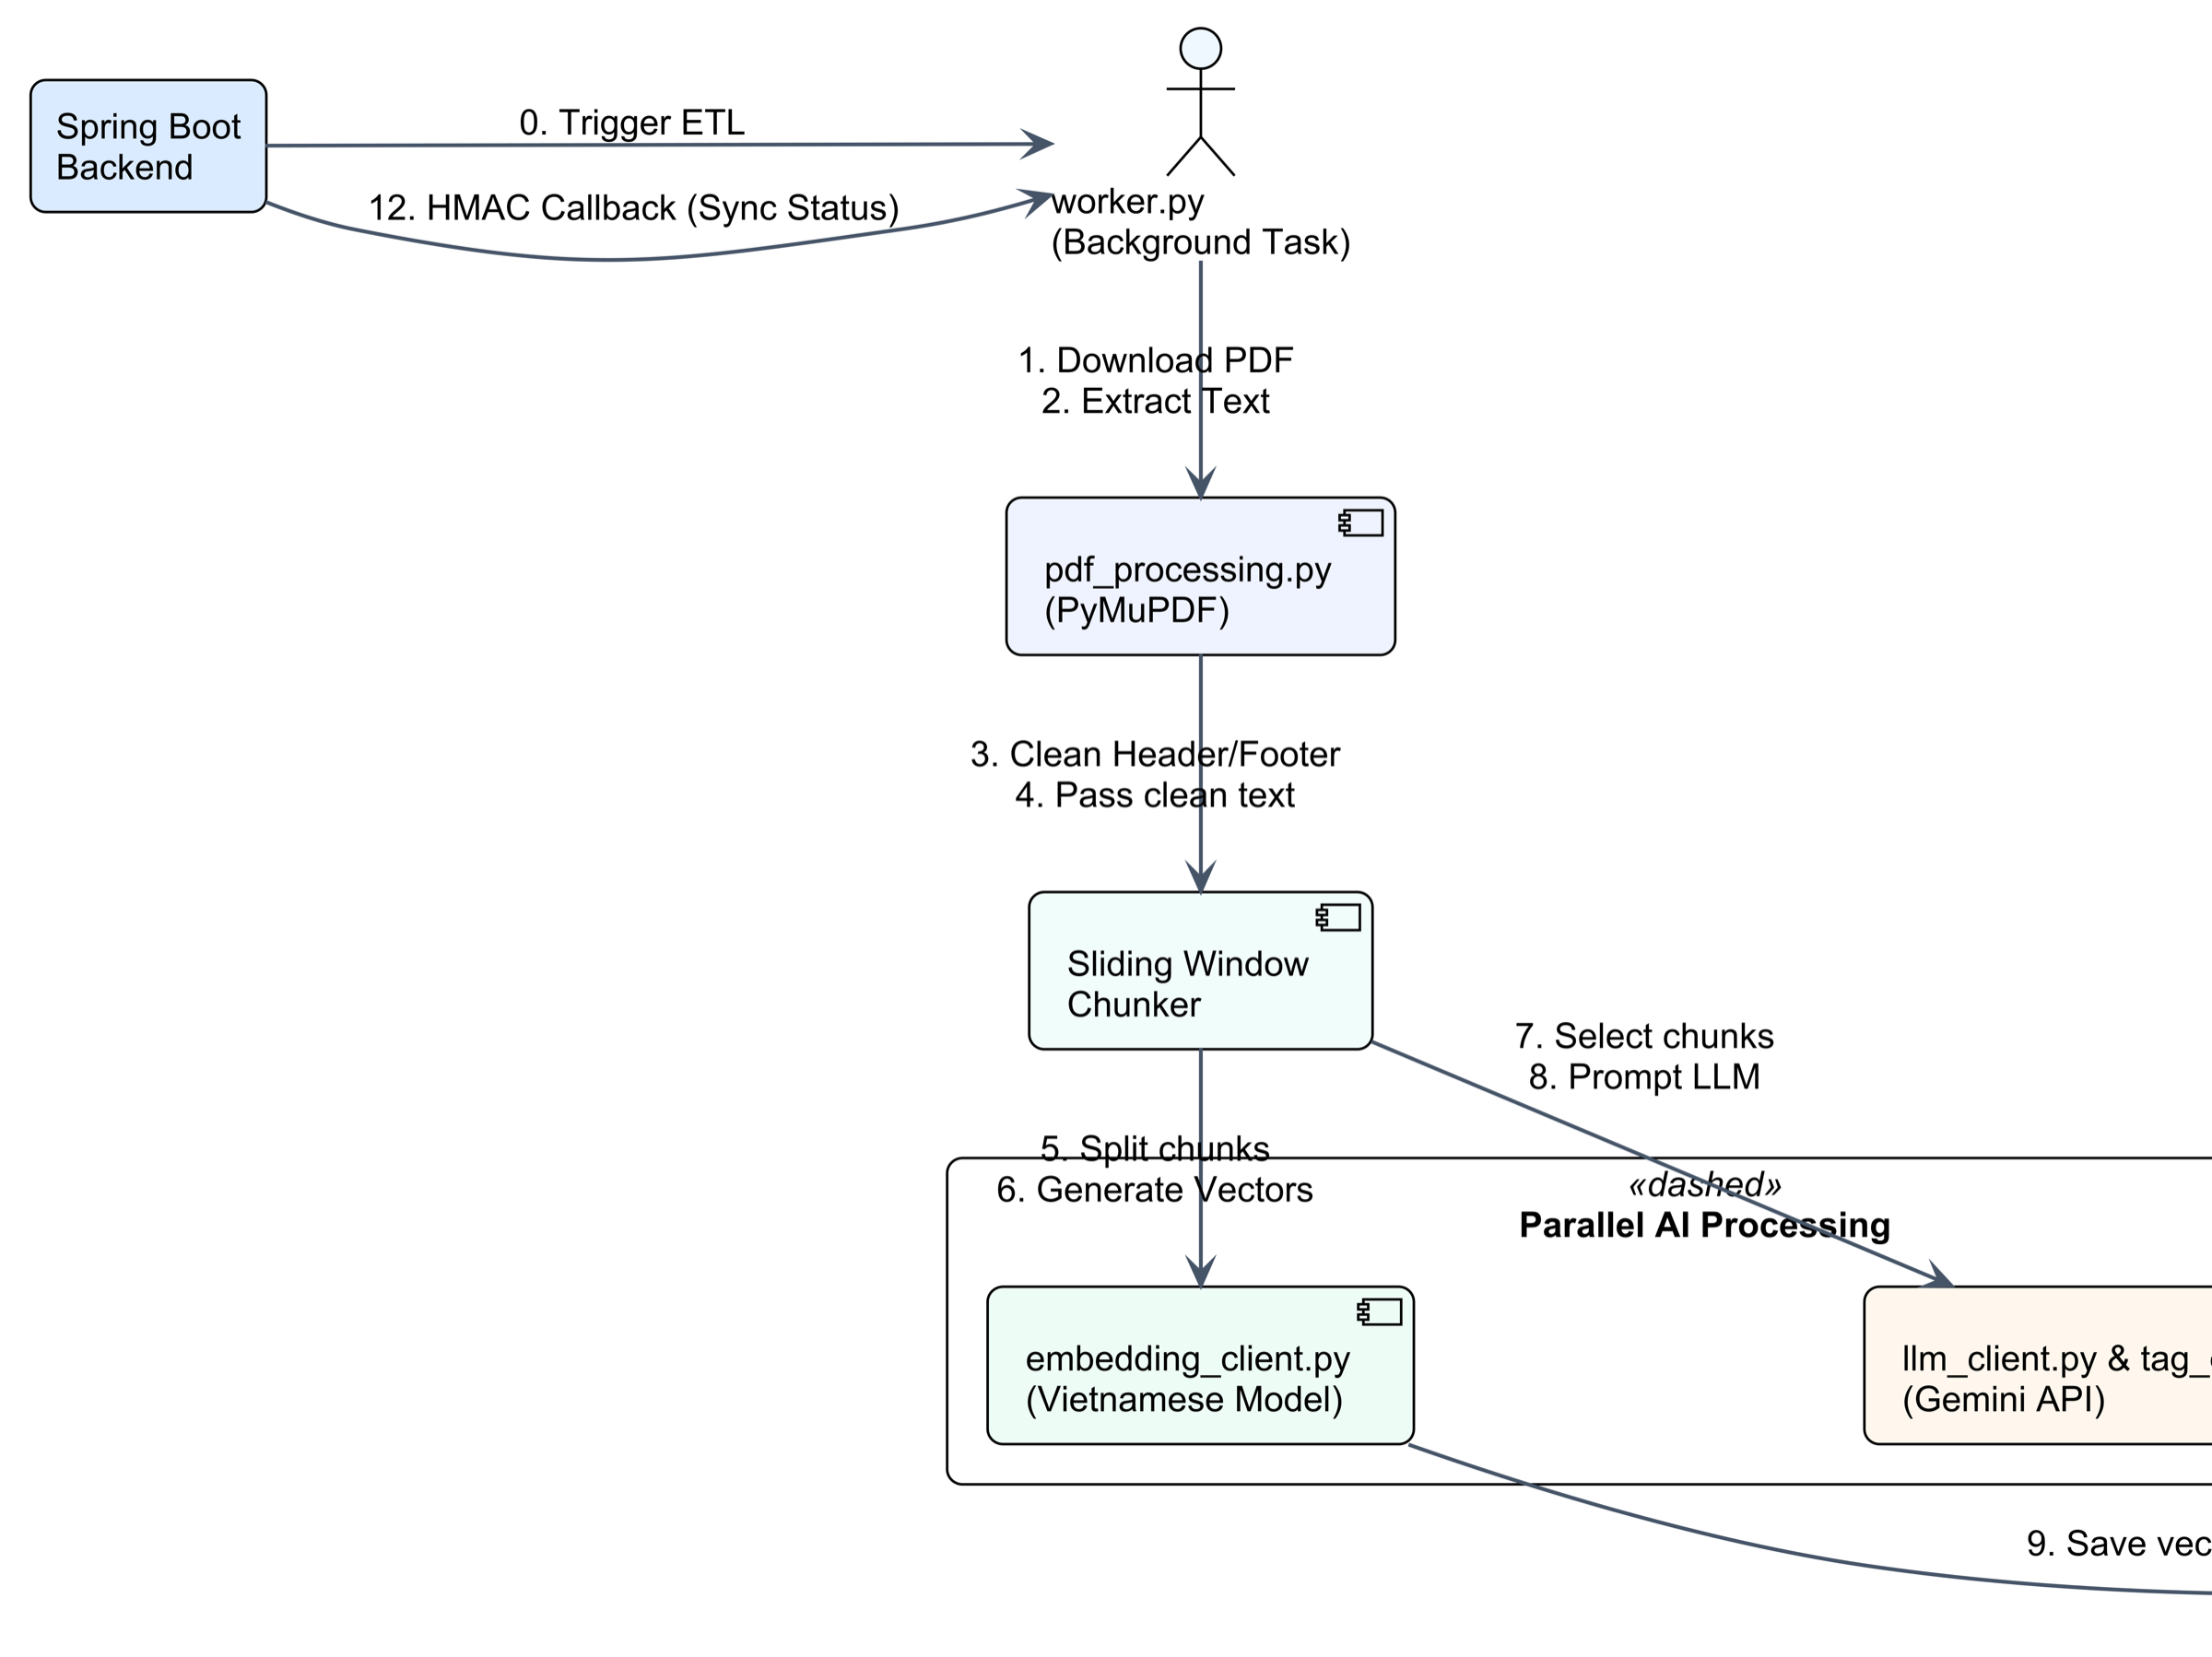
\includegraphics[width=0.52\textwidth]{figures/ch06/ai/ai_etl_pipeline.png}
    \caption{Luồng xử lý trích xuất, biến đổi và tải dữ liệu (ETL Pipeline) cho tài liệu PDF}
    \label{fig:ai_etl_pipeline}
\end{figure}

Chi tiết về chức năng và nhiệm vụ cụ thể của từng thành phần mã nguồn bên trong AI Service được thống kê tại Bảng \ref{tab:ai_components_implemented}.

% ================= NỐI TIẾP BẰNG BẢNG CỦA BẠN =================

\begin{longtable}{|p{3.8cm}|p{4cm}|p{6.5cm}|}
\caption{Các thành phần AI Service đã hiện thực}
\label{tab:ai_components_implemented}\\
\hline
\textbf{Thành phần} & \textbf{Nhóm chức năng} & \textbf{Nội dung đã hiện thực} \\
\hline
\endfirsthead
\hline
\textbf{Thành phần} & \textbf{Nhóm chức năng} & \textbf{Nội dung đã hiện thực} \\
\hline
\endhead
\texttt{api\_service.py} & FastAPI gateway &
Cung cấp health check, semantic search, similar publications, recommendation và
xử lý publication theo request đồng bộ. \\
\hline
\texttt{worker.py} & Xử lý nền &
Nhận message xử lý sách, tải PDF, chạy ETL, ghi trạng thái và gửi callback về
backend bằng chữ ký HMAC. \\
\hline
\texttt{pdf\_processing.py} & PDF ETL &
Tải/đọc PDF, trích xuất text bằng PyMuPDF, làm sạch header/footer/số trang, chia
chunk sliding window. \\
\hline
\texttt{pipeline.py} & Điều phối ETL &
Hash skip, sinh embedding, chọn chunk đại diện, reduce metadata bằng LLM, fallback
local khi lỗi và ghi kết quả vào database. \\
\hline
\texttt{embedding\_client.py} & Embedding &
Load SentenceTransformer tiếng Việt, sinh vector 768 chiều, normalize vector và
phục vụ semantic search/similar/recommendation. \\
\hline
\texttt{llm\_client.py} & Metadata AI &
Gọi Gemini, throttle/retry, ép output JSON, sinh summary, audience, tag tiếng
Việt và alias \texttt{tags\_en}. \\
\hline
\texttt{tag\_quality.py} & Làm sạch tag &
Lọc tag rác, chuẩn hóa alias Anh--Việt, map tag tiếng Việt sang thuật ngữ tiếng
Anh để hỗ trợ tìm kiếm song ngữ. \\
\hline
\texttt{recommender.py} & Gợi ý sách &
Huấn luyện ALS implicit feedback, kết hợp content-based, collaborative signal và
trending fallback. \\
\hline
\texttt{init\_schema.sql} & Dữ liệu AI &
Khởi tạo schema \texttt{ai\_engine}, bảng vector, ETL run, search log, index
pgvector và bảng recommendation. \\
\hline
\end{longtable}

% --- ĐOẠN CHUYỂN Ý 1: TỪ MODULE SANG MINH CHỨNG HÌNH ẢNH ---
Để minh chứng cho hoạt động của các thành phần mã nguồn nêu trên, hệ thống ghi nhận các kết quả đầu ra rõ rệt ở cả lớp giao diện người dùng lẫn lớp lưu trữ dữ liệu. Hình \ref{fig:ai_feature_showcase} thể hiện trải nghiệm trực quan của bạn đọc khi sử dụng công cụ tìm kiếm ngữ nghĩa và tiếp nhận các đề xuất sách cá nhân hóa. Song song đó, Hình \ref{fig:ai_etl_vector_showcase} cung cấp bằng chứng kỹ thuật (Technical Evidence) về tiến trình xử lý nền (ETL run) và cấu trúc dữ liệu vector nhiều chiều đã được lưu trữ thành công trong \texttt{pgvector}.

\begin{figure}[H]
    \centering
    \begin{subfigure}[b]{0.48\textwidth}
        \centering
        \includegraphics[width=\linewidth]{figures/ch06/ai/semantic_search.png}
        \caption{Semantic search}
    \end{subfigure}
    \hfill
    \begin{subfigure}[b]{0.48\textwidth}
        \centering
        \includegraphics[width=\linewidth]{figures/ch06/ai/recommendation.png}
        \caption{Gợi ý sách}
    \end{subfigure}
    \caption{Các chức năng AI đã tích hợp vào hệ thống}
    \label{fig:ai_feature_showcase}
\end{figure}

\begin{figure}[H]
    \centering
    \begin{subfigure}[b]{0.48\textwidth}
        \centering
        \includegraphics[width=\linewidth]{figures/ch06/ai/etl_run.png}
        \caption{Kết quả chạy ETL}
    \end{subfigure}
    \hfill
    \begin{subfigure}[b]{0.48\textwidth}
        \centering
        \includegraphics[width=\linewidth]{figures/ch06/ai/vector_db.png}
        \caption{Dữ liệu vector trong PostgreSQL}
    \end{subfigure}
    \caption{Pipeline xử lý PDF và lưu vector}
    \label{fig:ai_etl_vector_showcase}
\end{figure}

% --- ĐOẠN CHUYỂN Ý 2: TỪ HÌNH ẢNH SANG NĂNG LỰC KỸ THUẬT ---
Dựa trên các kết quả trực quan này, Bảng \ref{tab:ai_capability_summary} tổng hợp chi tiết các năng lực trí tuệ nhân tạo cốt lõi mà phân hệ AI Service đã đảm nhiệm. Các năng lực này được thiết kế không chỉ để phô diễn công nghệ, mà còn phải đáp ứng nghiêm ngặt các tiêu chuẩn về an toàn tích hợp, khả năng chịu lỗi (fault tolerance) và cơ chế dự phòng (fallback) khi giao tiếp với mô hình ngôn ngữ lớn (LLM).

\begin{table}[H]
\centering
\small
\begin{tabularx}{\textwidth}{|p{3.5cm}|X|}
\hline
\textbf{Năng lực AI} & \textbf{Nội dung đã hiện thực} \\
\hline
Xử lý PDF &
Upload PDF từ thủ thư, chạy ETL nền, lưu trạng thái \texttt{RUNNING},
\texttt{SUCCESS}, \texttt{FAILED}, không làm gián đoạn nghiệp vụ catalog. \\
\hline
Semantic search &
Sinh embedding cho truy vấn, tìm chunk gần nhất bằng pgvector, gom về
publication id và trả kết quả cho backend lọc nghiệp vụ. \\
\hline
Metadata enrichment &
Sinh summary, audience, tag học thuật, alias tiếng Anh và ghi về publication để
hiển thị trên chi tiết sách/tìm kiếm. \\
\hline
Similar books &
Tính tương đồng dựa trên vector nội dung và metadata để đề xuất sách liên quan
từ trang chi tiết. \\
\hline
Recommendation &
Gợi ý cá nhân hóa theo lịch sử xem, wishlist, mượn, rating; có fallback khi
người dùng mới hoặc dữ liệu tương tác còn ít. \\
\hline
An toàn tích hợp &
Callback HMAC, timeout/retry, fallback local khi LLM lỗi, kiểm thử API contract
và kiểm tra độ trễ cơ bản. \\
\hline
\end{tabularx}
\caption{Các năng lực AI đã tích hợp vào hệ thống}
\label{tab:ai_capability_summary}
\end{table}

% --- ĐOẠN CHUYỂN Ý 3: TỪ KỸ THUẬT SANG GIÁ TRỊ VẬN HÀNH ---
Công nghệ chỉ thực sự có ý nghĩa khi nó phục vụ đúng bài toán con người. Bảng \ref{tab:ai_value_highlights} đúc kết những điểm sáng nổi bật nhất, minh chứng cho việc ứng dụng AI đã thực sự giải phóng sức lao động của thủ thư (thông qua tự động hóa xử lý nền) và nâng tầm trải nghiệm khám phá tri thức của độc giả (thông qua tìm kiếm trên lõi nội dung thay vì từ khóa bề mặt).

\begin{table}[H]
\centering
\small
\begin{tabularx}{\textwidth}{|p{3.4cm}|X|p{3.4cm}|}
\hline
\textbf{Điểm hiện thực} & \textbf{Nội dung đã làm} & \textbf{Giá trị thực tế} \\
\hline
Xử lý nền &
AI worker nhận request, tải PDF, chạy ETL và callback kết quả về backend. &
Thủ thư không phải chờ AI xử lý xong mới tiếp tục thao tác catalog. \\
\hline
Tìm trên nội dung PDF &
Chunk nội dung được embedding và lưu vào pgvector để semantic search. &
Kết quả tìm kiếm dựa trên nội dung sách, không chỉ tiêu đề hoặc mô tả. \\
\hline
Metadata enrichment &
Sinh summary, audience, tag tiếng Việt và alias tiếng Anh. &
Trang chi tiết sách và bộ lọc tìm kiếm có thêm dữ liệu có ích cho người đọc. \\
\hline
Fallback &
Khi LLM lỗi hoặc dữ liệu tương tác ít, hệ thống dùng rule local, content-based và trending. &
Tính năng AI vẫn có kết quả ổn định trong điều kiện demo hoặc quota giới hạn. \\
\hline
\end{tabularx}
\caption{Các điểm giá trị nổi bật ở AI Service}
\label{tab:ai_value_highlights}
\end{table}

% --- ĐOẠN CHUYỂN Ý 4: TỔNG KẾT TOÀN BỘ CHƯƠNG 6 ---
\subsection{Tổng kết kết quả hiện thực}

Khép lại toàn bộ quá trình triển khai từ Frontend, Backend đến AI Service, sự thành công của một hệ thống phần mềm không chỉ nằm ở việc hoàn thiện từng module đơn lẻ, mà là khả năng liên kết chúng thành các luồng nghiệp vụ (Business Flows) thông suốt.

Bảng \ref{tab:implementation_value_flows} tổng hợp 4 luồng giá trị xương sống của dự án, đối chiếu trực tiếp giữa các thành phần công nghệ đã tham gia và những minh chứng rõ nét đã được trình bày xuyên suốt chương này. Đây là thước đo cuối cùng khẳng định hệ thống đã được xây dựng hoàn chỉnh từ đầu đến cuối (end-to-end) và đáp ứng trọn vẹn bài toán thực tiễn đặt ra ban đầu.

\begin{table}[H]
\centering
\small
\begin{tabularx}{\textwidth}{|p{3.4cm}|X|p{3.4cm}|}
\hline
\textbf{Luồng được show} & \textbf{Thành phần tham gia} & \textbf{Kết quả thể hiện trong Chương 6} \\
\hline
Upload và xử lý sách &
Frontend upload, Backend catalog/AI gateway, AI worker, pgvector. &
Có màn hình upload, bảng module, ảnh ETL, ảnh vector DB và callback. \\
\hline
Tìm kiếm thông minh &
Public search UI, Backend search API, AI semantic search, catalog filter. &
Có màn hình tìm kiếm, bảng năng lực AI và ảnh semantic search. \\
\hline
Mượn--trả và thanh toán &
User/librarian UI, circulation module, PayOS, notification realtime. &
Có màn hình dashboard, mượn sách, QR PayOS, cập nhật thanh toán và notification. \\
\hline
Quản trị vận hành &
Admin/librarian pages, audit/policy, scheduler, API documentation. &
Có bảng module Backend, bảng giá trị Backend và ảnh Swagger/cấu trúc module. \\
\hline
\end{tabularx}
\caption{Các luồng giá trị được minh chứng trong phần hiện thực}
\label{tab:implementation_value_flows}
\end{table}

\section{Tổng kết hiện thực}

Về tổng thể, hệ thống đã được hiện thực theo đúng ba lớp: frontend phục vụ tương
tác theo vai trò, backend giữ nghiệp vụ và dữ liệu gốc, AI service xử lý các tác
vụ thông minh. Các chức năng đã làm không chỉ dừng ở demo giao diện, mà đã nối
tới API, cơ sở dữ liệu, tác vụ nền, dịch vụ ngoài, kiểm thử và cấu hình triển
khai. Bảng dưới đây tóm tắt các luồng end-to-end quan trọng nhất.

\begin{table}[H]
\centering
\small
\begin{tabularx}{\textwidth}{|p{3.7cm}|X|}
\hline
\textbf{Luồng end-to-end} & \textbf{Các phần đã nối thông} \\
\hline
Đăng ký/đăng nhập &
Frontend auth pages, backend auth module, email verification, JWT/refresh token,
Google OAuth2 và route guard theo role. \\
\hline
Tra cứu và mượn sách &
Public/user search, catalog API, trạng thái bản sao, circulation API, thông báo
cho bạn đọc và dashboard thủ thư. \\
\hline
Đặt trước &
User reservation page, backend reservation queue, scheduler deadline, xác nhận
nhận sách và notification realtime. \\
\hline
Phí phạt &
Fine API, giao diện bạn đọc/thủ thư, PayOS QR, thanh toán tiền mặt, cập nhật
trạng thái fine và lịch sử giao dịch. \\
\hline
Upload PDF và AI &
Librarian upload, presigned URL, backend AI gateway, worker ETL, Gemini metadata,
pgvector và callback cập nhật publication. \\
\hline
Tìm kiếm/gợi ý thông minh &
Semantic search UI, AI service, recommendation module, behavior tracking, similar
books và fallback khi dữ liệu ít. \\
\hline
Vận hành &
Admin policy, audit log, scheduler, WebSocket notification, Docker Compose,
Nginx reverse proxy và cấu hình môi trường production. \\
\hline
\end{tabularx}
\caption{Các luồng end-to-end đã hiện thực}
\label{tab:end_to_end_summary}
\end{table}

% \chapter{Kiểm thử hệ thống}
\label{ch:testing}

Chương này trình bày chiến lược kiểm thử và kết quả thực nghiệm của hệ thống
Library74. Mục tiêu của kiểm thử không chỉ là chứng minh chương trình chạy được,
mà là chứng minh các thành phần chính của hệ thống hoạt động ổn định ở nhiều
tầng khác nhau: logic mã nguồn, hợp đồng API, pipeline AI, môi trường triển khai
thật, bảo mật cơ bản và khả năng chịu tải có kiểm soát.

Chiến lược kiểm thử được tổ chức theo dạng phễu. Ở tầng dưới, các unit test và
contract test chạy nhanh để bắt lỗi hồi quy trong mã nguồn. Ở tầng giữa, các
integration test kiểm tra cơ sở dữ liệu, API contract và cơ chế fallback giữa
các service. Ở tầng trên, hệ thống được kiểm thử trực tiếp trên domain production
\texttt{https://library74.uk} để xác nhận phiên bản triển khai thật phản hồi ổn
định.

\section{Chiến lược và môi trường kiểm thử}

Các kịch bản kiểm thử được tách thành hai môi trường. Môi trường local tập trung
vào tính đúng đắn của mã nguồn và hợp đồng dữ liệu. Môi trường production tập trung
vào khả năng vận hành thực tế sau khi hệ thống được đóng gói bằng Docker và đưa
lên server.

\begin{table}[H]
\centering
\scriptsize
\renewcommand{\arraystretch}{1.35}
\begin{tabularx}{\textwidth}{|p{2.9cm}|p{3.6cm}|p{2.8cm}|X|}
\hline
\textbf{Tầng kiểm thử} & \textbf{Mục tiêu} & \textbf{Công cụ} & \textbf{Bằng chứng thực nghiệm} \\
\hline
Local unit/contract &
Bắt lỗi logic và hợp đồng dữ liệu trước khi triển khai. &
Jest, JUnit, Mockito, pytest &
Frontend 62/62 test pass; Backend 79/79 test pass; AI Service 72 pass, 3 skip. \\
\hline
Integration &
Kiểm tra tương tác giữa service, schema database và API contract. &
Spring Boot Test, Testcontainers, MockMvc &
Backend integration chạy với PostgreSQL thật; AI SQL contract kiểm schema \texttt{public}/\texttt{ai\_engine}. \\
\hline
Production smoke &
Xác nhận hệ thống thật phản hồi đúng trên domain public. &
Curl, Python smoke script &
Domain \texttt{library74.uk} trả HTTP/2 200, có security headers; 8/8 production smoke case pass. \\
\hline
AI benchmark &
Đo chất lượng AI bằng metric định lượng thay vì nhận xét cảm tính. &
\texttt{ai\_quality\_benchmark.py} &
Reliability 95.46/100; Search Recall@5 87.5\%; nDCG@5 0.907; Hallucination guard 100\%. \\
\hline
Security &
Kiểm tra endpoint nhạy cảm bị bảo vệ bởi xác thực và phân quyền. &
API smoke, controller contract &
Login sai bị từ chối; admin endpoint không token trả 401; HTTPS có HSTS/CSP/nosniff; callback AI có HMAC contract. \\
\hline
Load test &
Đo khả năng phục vụ request đọc dưới tải đồng thời có kiểm soát. &
Python load probe &
50/100/200 virtual users; cả ba mức đều đạt error 0.00\%; mức 100 users đạt 42.11 req/s, p95 4191.64ms; mức 200 users đạt p95 7678.82ms. \\
\hline
\end{tabularx}
\caption{Tổng quan chiến lược kiểm thử hệ thống}
\label{tab:testing_strategy_overview}
\end{table}

Trọng tâm của chương này là các bằng chứng có thể lặp lại. Các kết quả đều được
ghi thành ảnh hoặc log, sau đó nhúng trực tiếp vào báo cáo để tránh tình trạng
mô tả chung chung mà không có số liệu đi kèm.

\section{Kiểm thử tầng mã nguồn}

\subsection{Kiểm thử Frontend}

Frontend được kiểm thử bằng Jest, Testing Library và môi trường
\texttt{jsdom}. Bộ test tập trung vào những phần ảnh hưởng rộng đến trải nghiệm
người dùng: ngôn ngữ Việt--Anh, theme sáng/tối, trạng thái đăng nhập, upload,
notification, helper đặt trước, service contract và các component giao diện dùng
chung.

\begin{figure}[H]
    \centering
    \IfFileExists{figures/ch07/test-results/fe-jest-result.png}{
        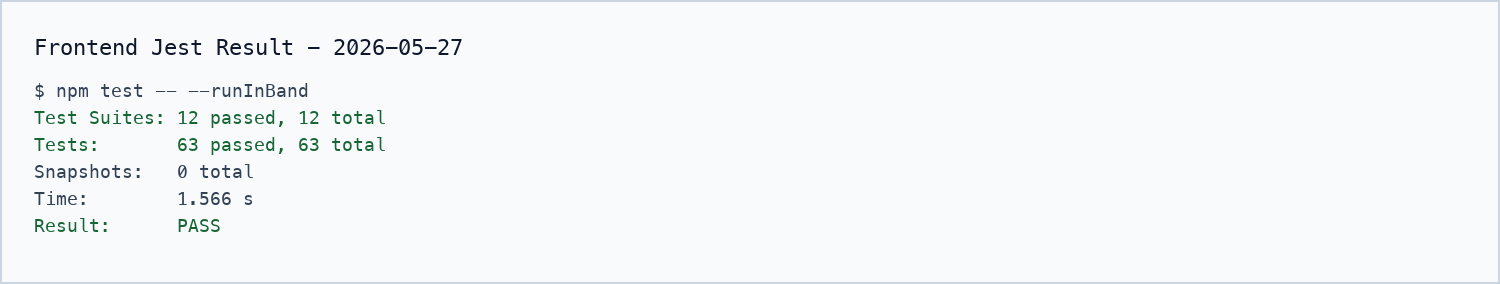
\includegraphics[width=0.9\textwidth]{figures/ch07/test-results/fe-jest-result.png}
    }{
        \fbox{\parbox[c][5cm][c]{0.9\textwidth}{\centering Thiếu ảnh kết quả Frontend tại \texttt{figures/ch07/test-results/fe-jest-result.png}}}
    }
    \caption{Kết quả chạy bộ kiểm thử Frontend}
    \label{fig:fe_unit_test_result}
\end{figure}

\begin{table}[H]
\centering
\small
\begin{tabularx}{\textwidth}{|p{4cm}|X|}
\hline
\textbf{Chỉ số} & \textbf{Kết quả} \\
\hline
Test suites & \textbf{12 passed / 12 total}. \\
\hline
Test cases & \textbf{62 passed / 62 total}. \\
\hline
Snapshot & \textbf{0 total}. \\
\hline
Thời gian chạy & Khoảng \textbf{1.31s}. \\
\hline
Kết luận & Frontend pass toàn bộ ở tầng unit, context, component và service contract. \\
\hline
\end{tabularx}
\caption{Kết quả kiểm thử Frontend}
\label{tab:fe_test_result}
\end{table}

Các test frontend giúp kiểm soát những lỗi dễ lan rộng trong SPA. Nếu
\texttt{LanguageContext} sai, nhiều màn hình có thể hiển thị sai ngôn ngữ. Nếu
\texttt{ThemeContext} sai, toàn bộ giao diện có thể lệch trạng thái sáng/tối.
Nếu service contract sai endpoint hoặc payload, frontend có thể lỗi ngay cả khi
giao diện vẫn render được. Vì vậy bộ test này đóng vai trò lớp phòng vệ đầu tiên
trước khi kiểm thử trên web thật.

\subsection{Kiểm thử Backend}

Backend được kiểm thử bằng JUnit 5, Mockito, MockMvc, Spring Boot Test và
Testcontainers. Các test được chia theo module nghiệp vụ: xác thực, người dùng,
catalog, mượn--trả, đặt trước, phí phạt, wishlist/rating, AI gateway và callback
từ AI service. Với các truy vấn native SQL quan trọng, PostgreSQL thật được dùng
trong container để tránh sai lệch so với database production.

\begin{figure}[H]
    \centering
    \IfFileExists{figures/ch07/test-results/be-test-result.png}{
        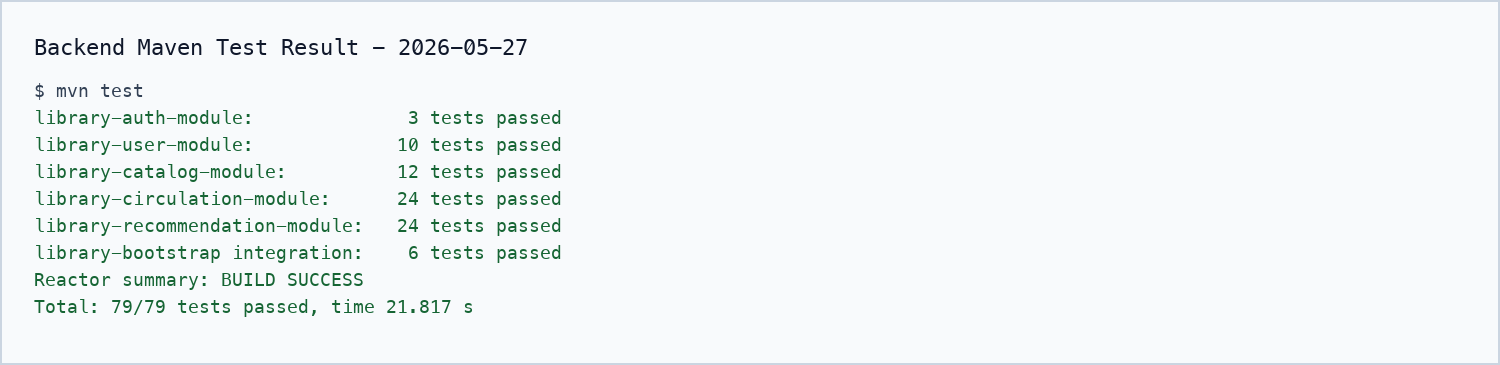
\includegraphics[width=0.9\textwidth]{figures/ch07/test-results/be-test-result.png}
    }{
        \fbox{\parbox[c][5cm][c]{0.9\textwidth}{\centering Thiếu ảnh kết quả Backend tại \texttt{figures/ch07/test-results/be-test-result.png}}}
    }
    \caption{Kết quả chạy bộ kiểm thử Backend}
    \label{fig:be_test_result}
\end{figure}

\begin{table}[H]
\centering
\small
\begin{tabularx}{\textwidth}{|p{4.2cm}|p{2cm}|p{2cm}|X|}
\hline
\textbf{Module} & \textbf{Class} & \textbf{Test} & \textbf{Nội dung kiểm thử chính} \\
\hline
\texttt{library-auth-module} & 1 & 3 & Đăng ký, validation email/student id và payload hợp lệ. \\
\hline
\texttt{library-user-module} & 3 & 10 & Signup, notification page, unread count, mark read và mark all read. \\
\hline
\texttt{library-catalog-module} & 5 & 12 & Tạo publication/item, upload URL, save document URL, public search SQL và publication controller. \\
\hline
\texttt{library-circulation-module} & 5 & 24 & Borrow request, return book, fine, reservation, transaction controller và policy cấu hình từ DB. \\
\hline
\texttt{library-recommendation-module} & 7 & 24 & Wishlist, rating, AI gateway fallback, semantic/recommendation contract và signed AI callback. \\
\hline
\texttt{library-bootstrap} & 2 & 6 & Integration với PostgreSQL thật cho borrow/return flow và reservation SQL. \\
\hline
\textbf{Tổng cộng} & \textbf{23} & \textbf{79} & \textbf{79/79 test pass}. \\
\hline
\end{tabularx}
\caption{Phạm vi kiểm thử Backend theo module}
\label{tab:be_test_modules}
\end{table}

Bộ test backend chứng minh các use case lõi hoạt động đúng: quản lý ấn phẩm,
tìm kiếm public, xác thực, notification, mượn--trả, đặt trước, thanh toán/phí
phạt, đánh giá sách, wishlist và tích hợp AI. Các test controller kiểm request
binding, validation và response JSON; các test use case kiểm nhánh nghiệp vụ và
fallback; các test integration kiểm migration và truy vấn trên PostgreSQL thật.

\subsection{Kiểm thử AI Service}

AI Service được kiểm thử ở hai mức: contract/regression test và quality
benchmark. Contract test dùng \texttt{pytest} để kiểm tra pipeline xử lý PDF,
chunking, parse JSON từ LLM, fallback, tag quality, SQL contract, semantic
search, recommender và chữ ký HMAC callback.

\begin{figure}[H]
    \centering
    \IfFileExists{figures/ch07/test-results/ai-pytest-result.png}{
        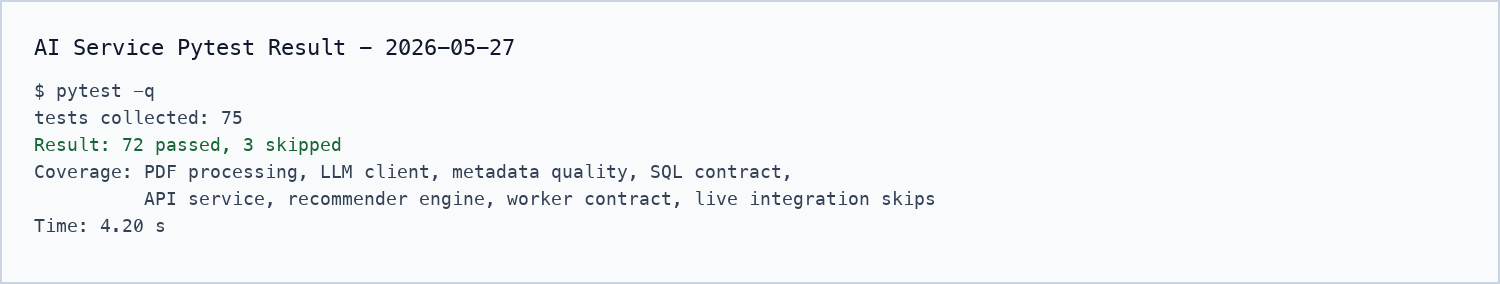
\includegraphics[width=0.9\textwidth]{figures/ch07/test-results/ai-pytest-result.png}
    }{
        \fbox{\parbox[c][5cm][c]{0.9\textwidth}{\centering Thiếu ảnh kết quả AI pytest tại \texttt{figures/ch07/test-results/ai-pytest-result.png}}}
    }
    \caption{Kết quả chạy bộ kiểm thử AI Service}
    \label{fig:ai_pytest_result}
\end{figure}

\begin{table}[H]
\centering
\small
\renewcommand{\arraystretch}{1.35}
\begin{tabularx}{\textwidth}{|p{4cm}|X|p{1.4cm}|}
\hline
\textbf{Hạng mục test} & \textbf{Nội dung xác thực} & \textbf{Case} \\
\hline
\texttt{pdf\_processing} và \texttt{pipeline\_core} & Làm sạch header/footer, bỏ ký tự lỗi, OCR sampling, chunk id ổn định, chọn representative chunks, budget reduce và fallback khi LLM lỗi. & 18 \\
\hline
\texttt{llm\_client}, metadata và benchmark helpers & Parse JSON, lọc tag generic, reject summary chỉ lặp catalog, giữ alias \texttt{tags\_en} 1--1 và tính Precision/Recall/MRR/nDCG. & 26 \\
\hline
\texttt{database\_sql\_contract} và config & Kiểm schema vector, publication tags, tag translations, điều kiện đủ AI output và cấu hình fallback. & 7 \\
\hline
\texttt{api\_service} & pgvector literal, tokenize tiếng Việt không dấu, hybrid search, ranking guard, recommendation fallback và giới hạn semantic result. & 13 \\
\hline
\texttt{recommender} và worker & ALS bundle, cold user, weighted interactions, Celery payload, download PDF và HMAC callback. & 8 \\
\hline
\texttt{integration\_live} & Health, semantic search và recommendation contract/latency với API thật; skip mặc định. & 3 skip \\
\hline
\textbf{Tổng cộng} & \textbf{72 pass, 3 skip} & \textbf{75} \\
\hline
\end{tabularx}
\caption{Phạm vi kiểm thử AI Service}
\label{tab:ai_contract_test_scope}
\end{table}

Bộ kiểm thử AI không phụ thuộc cảm tính. Các trường hợp LLM lỗi, JSON sai, tag
quá chung, summary lệch domain, SQL ghi sai schema hoặc callback thiếu chữ ký
đều được đưa vào test tự động. Nhờ vậy, pipeline AI có cơ chế kiểm soát trước
khi chạy trên tài liệu thật.

\section{Kiểm thử trên môi trường triển khai}

Hệ thống được triển khai trên môi trường thực tế tại tên miền \texttt{https://library74.uk}. Kiến trúc hạ tầng được đóng gói thông qua Docker Compose, vận hành song song các dịch vụ: Caddy làm máy chủ định tuyến ngược, Nginx, Spring Boot, FastAPI, Celery và hệ sinh thái trung gian (PostgreSQL pgvector, RabbitMQ, Kafka). Kết quả kiểm tra sức khỏe toàn cục xác nhận toàn bộ luồng giao tiếp giữa các container hoạt động ổn định.

\subsection{Kiểm thử tương tác hệ thống}

Các kịch bản smoke test được thiết kế dưới dạng luồng dữ liệu chỉ đọc, nhằm xác thực tính toàn vẹn của đường truyền từ trình duyệt qua máy chủ định tuyến ngược đến backend và phân hệ AI.

\begin{figure}[H]
    \centering
    \IfFileExists{figures/ch07/test-results/production-smoke-result.png}{
        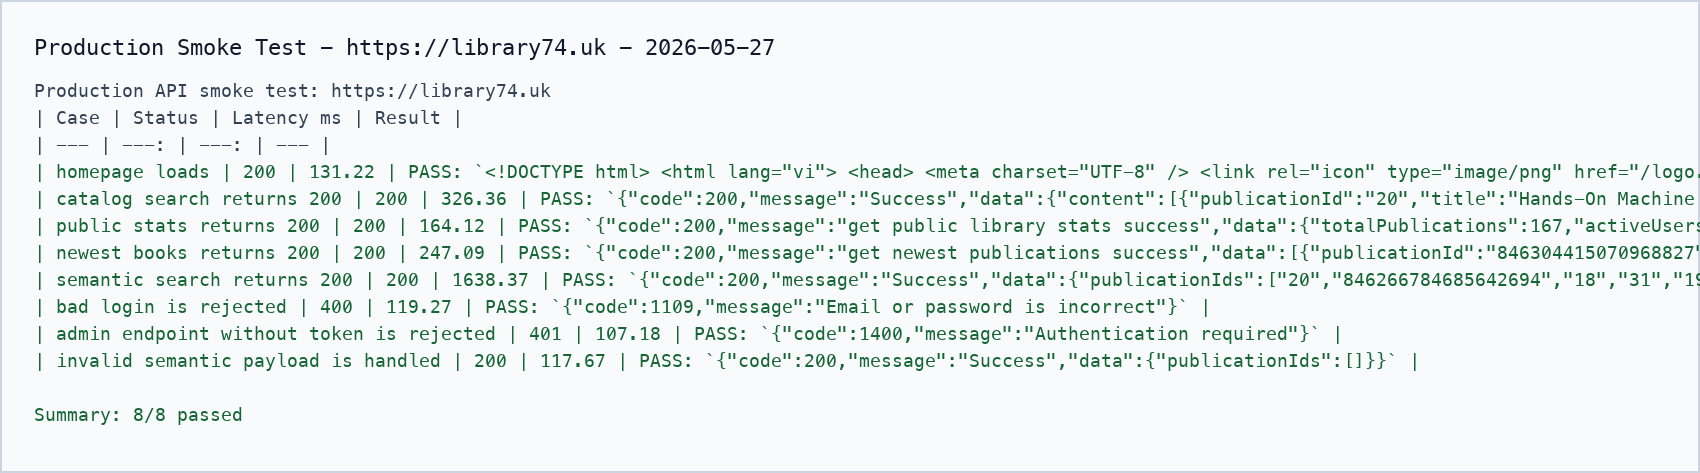
\includegraphics[width=0.95\textwidth]{figures/ch07/test-results/production-smoke-result.png}
    }{
        \fbox{\parbox[c][5cm][c]{0.9\textwidth}{\centering Thiếu ảnh production smoke test tại \texttt{figures/ch07/test-results/production-smoke-result.png}}}
    }
    \caption{Kết quả kiểm thử tương tác trên hệ thống \texttt{library74.uk}}
    \label{fig:production_smoke_result}
\end{figure}

\begin{table}[H]
\centering
\small
\renewcommand{\arraystretch}{1.3}
\begin{tabularx}{\textwidth}{|p{5cm}|p{2cm}|p{2.5cm}|X|}
\hline
\textbf{Kịch bản thao tác} & \textbf{Mã HTTP} & \textbf{Độ trễ} & \textbf{Trạng thái xử lý} \\
\hline
Tải tài nguyên trang chủ & 200 & 95.58ms & Thành công, tải trang tức thời. \\
\hline
Khởi xuất dữ liệu thống kê & 200 & 251.25ms & Thành công, truy vấn tổng hợp hoạt động. \\
\hline
Tra cứu danh mục & 200 & 136.23ms & Thành công, tìm kiếm từ khóa mượt mà. \\
\hline
Tìm kiếm ngữ nghĩa & 200 & 344.91ms & Thành công, AI Gateway phản hồi nhanh chóng. \\
\hline
Ràng buộc đăng nhập sai & 400 & 135.29ms & Bắt lỗi hợp lệ, từ chối cấp token. \\
\hline
Lọc quyền quản trị & 401 & 120.12ms & Thành công, tường lửa xác thực hoạt động. \\
\hline
Tiêm cấu trúc dữ liệu lỗi & 200 & 100.85ms & Thành công, bắt lỗi payload, không sập dịch vụ. \\
\hline
\multicolumn{4}{|c|}{\textbf{Kết luận: 100\% kịch bản vượt qua quy trình kiểm thử trên môi trường thực tế.}} \\
\hline
\end{tabularx}
\caption{Kết quả API smoke test trên phân hệ máy chủ}
\label{tab:production_smoke_result}
\end{table}

Ngoài bộ thử nghiệm tổng quát, hệ thống tiếp tục khẳng định tính đúng đắn ở luồng người dùng ẩn danh. Các tác vụ nâng cao như tìm kiếm ngữ nghĩa tiếng Việt (ví dụ: truy xuất nội dung "môi trường") và đề xuất sách tương tự đều được trả về chính xác mà không yêu cầu phiên đăng nhập, chứng minh chiến lược phân quyền tài nguyên mở được thiết lập chuẩn xác.

\subsection{Cấu trúc bảo mật định tuyến}

Chiến lược bảo mật được thiết lập đa tầng, bao phủ từ lớp mã nguồn đến cấu trúc vận hành máy chủ. Ở tầng quản trị nội dung, các endpoint nhạy cảm đều chịu sự giám sát của bộ lọc xác thực; thao tác thất bại sẽ bị chặn bằng mã lỗi nghiệp vụ chuẩn hóa. Phân hệ AI giao tiếp với máy chủ trung tâm thông qua luồng callback bọc chữ ký HMAC, loại bỏ nguy cơ giả mạo tiến trình.

Trên mặt trận giao thức mạng, cấu hình máy chủ định tuyến ngược tại lớp ngoài cùng tuân thủ nghiêm ngặt các tiêu chuẩn bảo mật quốc tế.

\begin{table}[H]
\centering
\small
\renewcommand{\arraystretch}{1.3}
\begin{tabularx}{\textwidth}{|p{4.2cm}|X|p{3.2cm}|}
\hline
\textbf{Nhóm rủi ro} & \textbf{Phương pháp kiểm soát} & \textbf{Kết quả thực nghiệm} \\
\hline
Leo thang đặc quyền & Khảo sát quyền truy cập quản trị khi không cung cấp JWT. & Chặn truy cập (HTTP 401). \\
\hline
Tấn công dò mật khẩu & Truyền tải thông tin đăng nhập sai cấu trúc liên tục. & Từ chối giao dịch. \\
\hline
Phá hoại quy trình AI & Gửi tập lệnh thiếu biến số truy xuất vào hàng đợi AI. & Trả về rỗng, tiến trình không bị crash. \\
\hline
Cấy ghép mã độc & Phân tích cấu trúc tiêu đề phản hồi HTTP tại tên miền thật. & Kích hoạt HSTS, CSP, nosniff đầy đủ. \\
\hline
Tràn bộ nhớ đệm & Đánh giá chính sách bộ nhớ đệm trên tài nguyên tĩnh. & Tệp JS được băm định danh bất biến, HTML không lưu vết. \\
\hline
\end{tabularx}
\caption{Đánh giá năng lực bảo vệ trên môi trường thực tế}
\label{tab:security_smoke_test}
\end{table}

\subsection{Khả năng giám sát và đo lường}

Để hệ thống có khả năng tự phục hồi và theo dõi dài hạn, mạng lưới đo lường được thiết lập khép kín. Công cụ Spring Actuator được kích hoạt trên hệ sinh thái backend nhằm cung cấp điểm nối khai thác sức khỏe hệ thống. Đặc biệt, để ngăn chặn rò rỉ cấu trúc dữ liệu, các luồng phân tích số liệu được bảo mật nội bộ và chỉ định tuyến cục bộ cho Prometheus và cAdvisor; hoàn toàn vô hình với môi trường Internet công cộng.

\begin{table}[H]
\centering
\small
\renewcommand{\arraystretch}{1.3}
\begin{tabularx}{\textwidth}{|p{4cm}|X|p{3.4cm}|}
\hline
\textbf{Phân hệ giám sát} & \textbf{Chiến lược đo lường} & \textbf{Tình trạng vận hành} \\
\hline
Kiểm tra sức khỏe máy chủ & Truy vấn trạng thái qua môi trường HTTPS. & Hệ thống hoạt động. \\
\hline
An toàn cấu hình metric & Kiểm thử truy cập từ luồng mạng ngoại vi. & Hệ thống từ chối (HTTP 401). \\
\hline
Định tuyến Prometheus & Giám sát tình trạng luồng xử lý metric cục bộ trên server. & Luồng dữ liệu nội bộ ổn định. \\
\hline
Quản trị tài nguyên & Phân tích lượng RAM/CPU tiêu thụ thông qua Docker. & Backend duy trì < 600MB RAM, AI API < 400MB RAM. \\
\hline
\end{tabularx}
\caption{Đánh giá mạng lưới đo lường trên phân hệ production}
\label{tab:observability_result}
\end{table}

\section{Đánh giá định lượng chất lượng AI}

Các module AI trong hệ thống không được đánh giá thông qua các nhận định cảm tính. Hệ thống sử dụng kịch bản \texttt{ai\_quality\allowbreak\_benchmark.py} để trích xuất metadata từ PostgreSQL trên môi trường production, gọi trực tiếp vào endpoint \texttt{/api/v1/ai/\allowbreak semantic-search} và tính toán các độ đo chuẩn trong lĩnh vực Truy xuất thông tin.

\begin{figure}[H]
    \centering
    \IfFileExists{figures/ch07/test-results/ai-quality-benchmark-result.png}{
        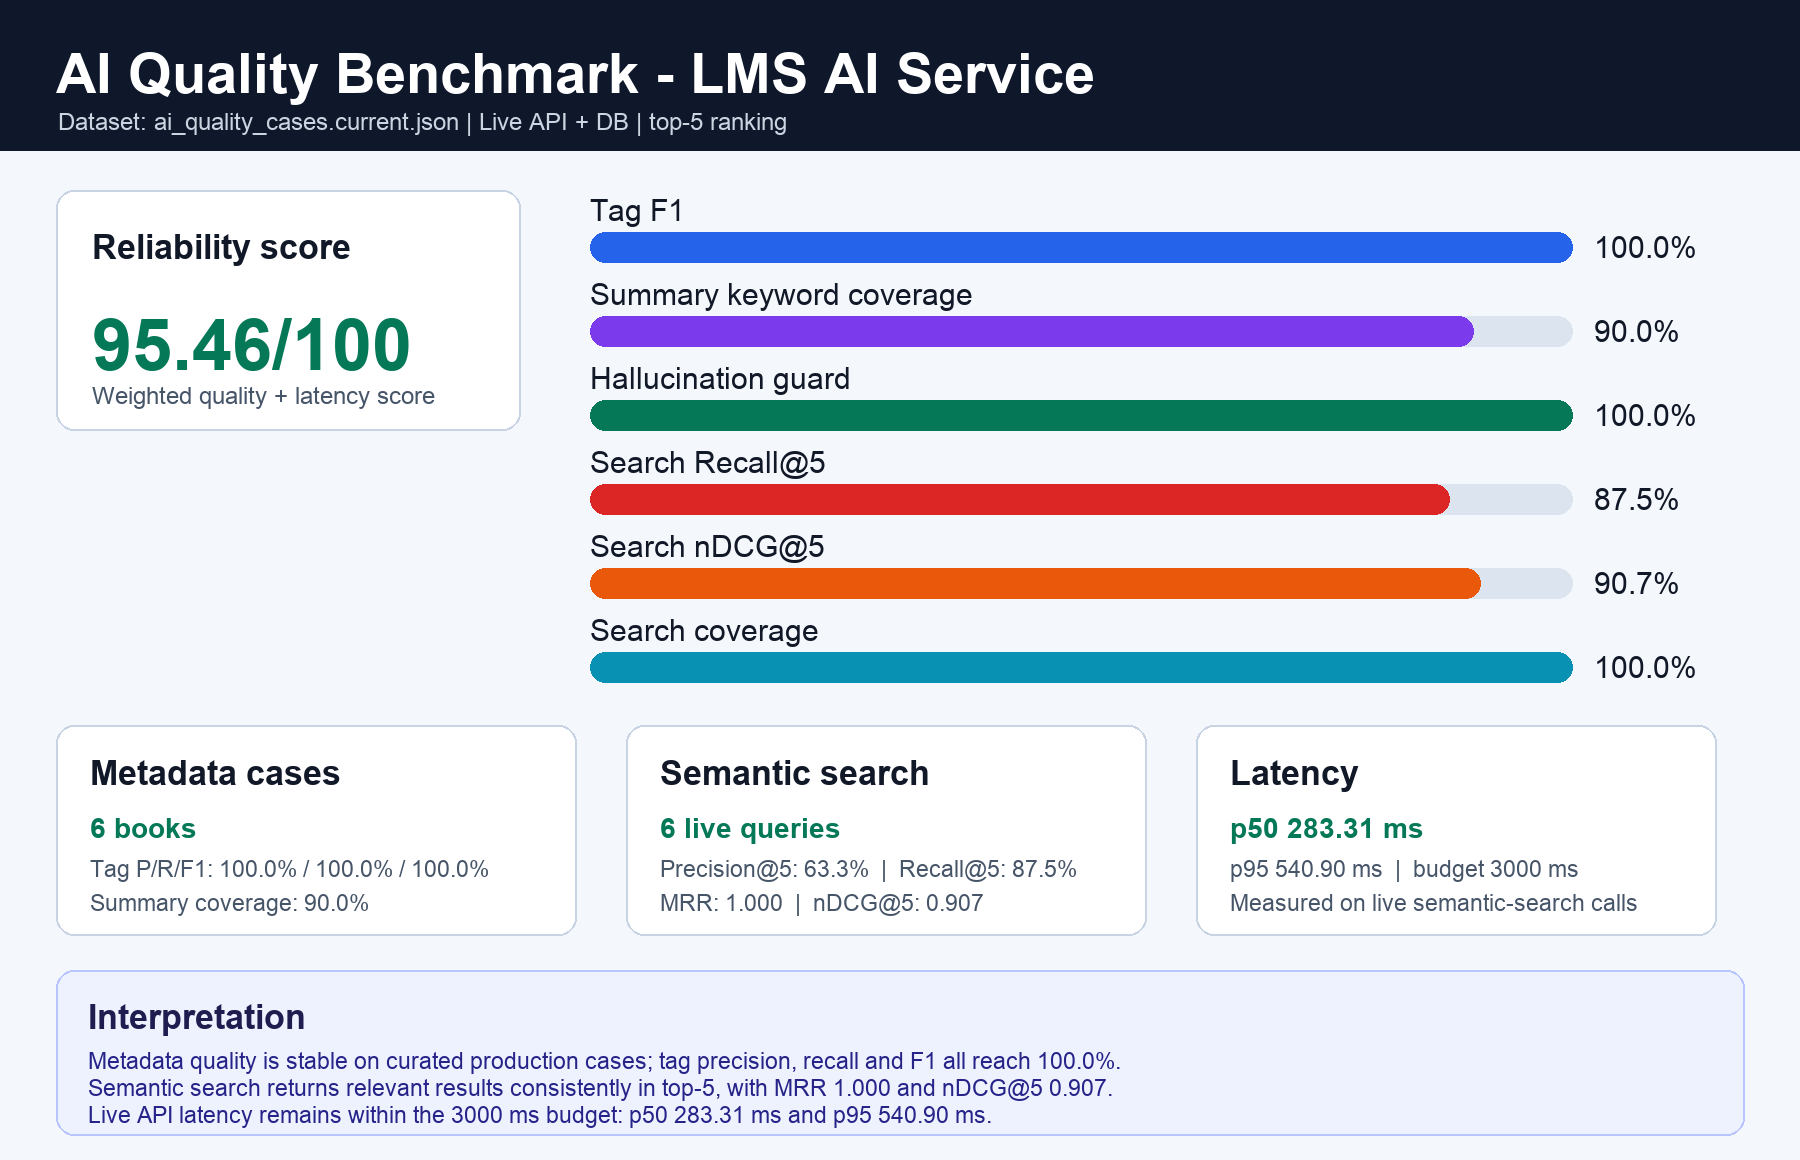
\includegraphics[width=0.95\textwidth]{figures/ch07/test-results/ai-quality-benchmark-result.png}
    }{
        \fbox{\parbox[c][5cm][c]{0.9\textwidth}{\centering Thiếu ảnh benchmark AI tại \texttt{figures/ch07/test-results/ai-quality-benchmark-result.png}}}
    }
    \caption{Kết quả benchmark định lượng chất lượng AI}
    \label{fig:ai_quality_benchmark_result}
\end{figure}

\begin{table}[H]
\centering
\small
\renewcommand{\arraystretch}{1.3}
\begin{tabularx}{\textwidth}{|p{3.6cm}|X|p{3.2cm}|}
\hline
\textbf{Hạng mục} & \textbf{Metric} & \textbf{Kết quả} \\
\hline
Reliability & Điểm tổng hợp có trọng số từ metadata, search và latency & \textbf{95.46/100} \\
\hline
Tag consistency & Precision / Recall / F1 so với tag curated trong production & \textbf{100.0\% / 100.0\% / 100.0\%} \\
\hline
Summary & Keyword coverage, length OK và hallucination guard & \textbf{90.0\%, 100.0\%, 100.0\%} \\
\hline
Semantic search & Precision@5, Recall@5, MRR và nDCG@5 & \textbf{63.3\%, 87.5\%, 1.000, 0.907} \\
\hline
Coverage & Tỉ lệ query trả về danh sách khác rỗng & \textbf{100.0\%} \\
\hline
Latency & p50 / p95 với budget 3000ms & \textbf{283.31ms / 540.90ms} \\
\hline
\end{tabularx}
\caption{Kết quả benchmark AI trên dữ liệu production hiện tại}
\label{tab:ai_quality_benchmark_result}
\end{table}

Với điểm tin cậy tổng hợp đạt \textbf{95.46/100}, hiệu năng thực tế của phân hệ AI được phân tích chi tiết qua các khía cạnh sau:

\begin{itemize}
    \item \textbf{Dữ liệu kiểm thử:} Bộ dữ liệu benchmark được tái thiết lập trực tiếp từ 6 ấn phẩm đặc thù đang lưu hành trên cơ sở dữ liệu production (trải dài qua các miền: môi trường, hóa học xanh, dầu khí, đại số tuyến tính, xác suất và polymer), đảm bảo độ tin cậy và bám sát thực tế vận hành.

    \item \textbf{Khả năng tìm kiếm ngữ nghĩa:} Đây tiếp tục là sức mạnh cốt lõi của hệ thống.
    \begin{itemize}
        \item \textit{Độ chính xác xếp hạng:} Đạt ngưỡng tuyệt đối với \texttt{MRR = 1.000} (kết quả đúng luôn xuất hiện ở vị trí đầu tiên) trên toàn bộ 6 truy vấn phức tạp (\texttt{Coverage = 100\%}).
        \item \textit{Phân bổ kết quả:} Các chỉ số \texttt{Recall@5 = 87.5\%} và \texttt{nDCG@5 = 0.907} chứng minh phần lớn tài liệu liên quan đều được ưu tiên đưa vào nhóm 5 kết quả đầu.
        \item \textit{Hiện tượng nhiễu dữ liệu:} Ở một số truy vấn ngách (ví dụ: "polymer/công nghệ nano"), hệ thống bắt đúng tài liệu đích ở vị trí đầu tiên, nhưng các vị trí tiếp theo bị nhiễu bởi sách vật liệu tổng quát, dẫn đến giảm nhẹ chỉ số \texttt{Precision@5}.
    \end{itemize}

    \item \textbf{Đúc kết và khai phá tri thức:}
    \begin{itemize}
        \item \textit{Khả năng tóm tắt:} Đáp ứng hoàn hảo tiêu chuẩn an toàn học thuật. Độ phủ từ khóa đạt \textbf{90.0\%}; 100\% bản tóm tắt vượt qua rào chắn chống ảo giác và tuân thủ giới hạn độ dài.
        \item \textit{Độ nhất quán của nhãn:} Đạt điểm tuyệt đối \texttt{F1-Score = 100\%}. Báo cáo nhìn nhận số liệu này đại diện cho sự nhất quán giữa metadata do AI sinh ra so với bộ nhãn đã được giám tuyển trên production, thay vì diễn giải sai lệch thành năng lực suy luận độc lập của mô hình trên tài liệu lạ.
    \end{itemize}

    \item \textbf{Tốc độ phản hồi:} Hệ thống tối ưu hóa thành công đường truyền với \texttt{p95 latency} chỉ đạt \textbf{540.90ms}, vượt xa ngân sách giới hạn 3000ms, đảm bảo trải nghiệm tra cứu tức thời.

    \item \textbf{Hệ thống gợi ý:} Tạm thời không áp dụng chấm điểm định lượng do hệ thống đang ở giai đoạn khởi động nguội, chưa tích lũy đủ dữ liệu tương tác để tạo bộ hồ sơ người dùng chuẩn. Phân hệ hiện được bảo vệ vững chắc bởi các bài kiểm thử tự động kết hợp logic dự phòng, sẵn sàng đo lường các chỉ số \texttt{Precision@K} khi hệ thống thu thập đủ luồng hành vi từ người dùng thực tế.
\end{itemize}

\section{Kiểm thử chịu tải có kiểm soát}

Kiểm thử chịu tải được thực hiện trên endpoint đọc dữ liệu, không ghi dữ liệu
vào production. Endpoint được chọn là tìm kiếm catalog:
\texttt{/api/v1/publications/search?keyword=machine\&page=0\&limit=5}. Đây là
luồng có giá trị thực tế vì người dùng thường xuyên tìm kiếm sách, đồng thời
việc gọi endpoint này không làm thay đổi trạng thái nghiệp vụ.

\begin{figure}[H]
    \centering
    \IfFileExists{figures/ch07/test-results/production-load-result.png}{
        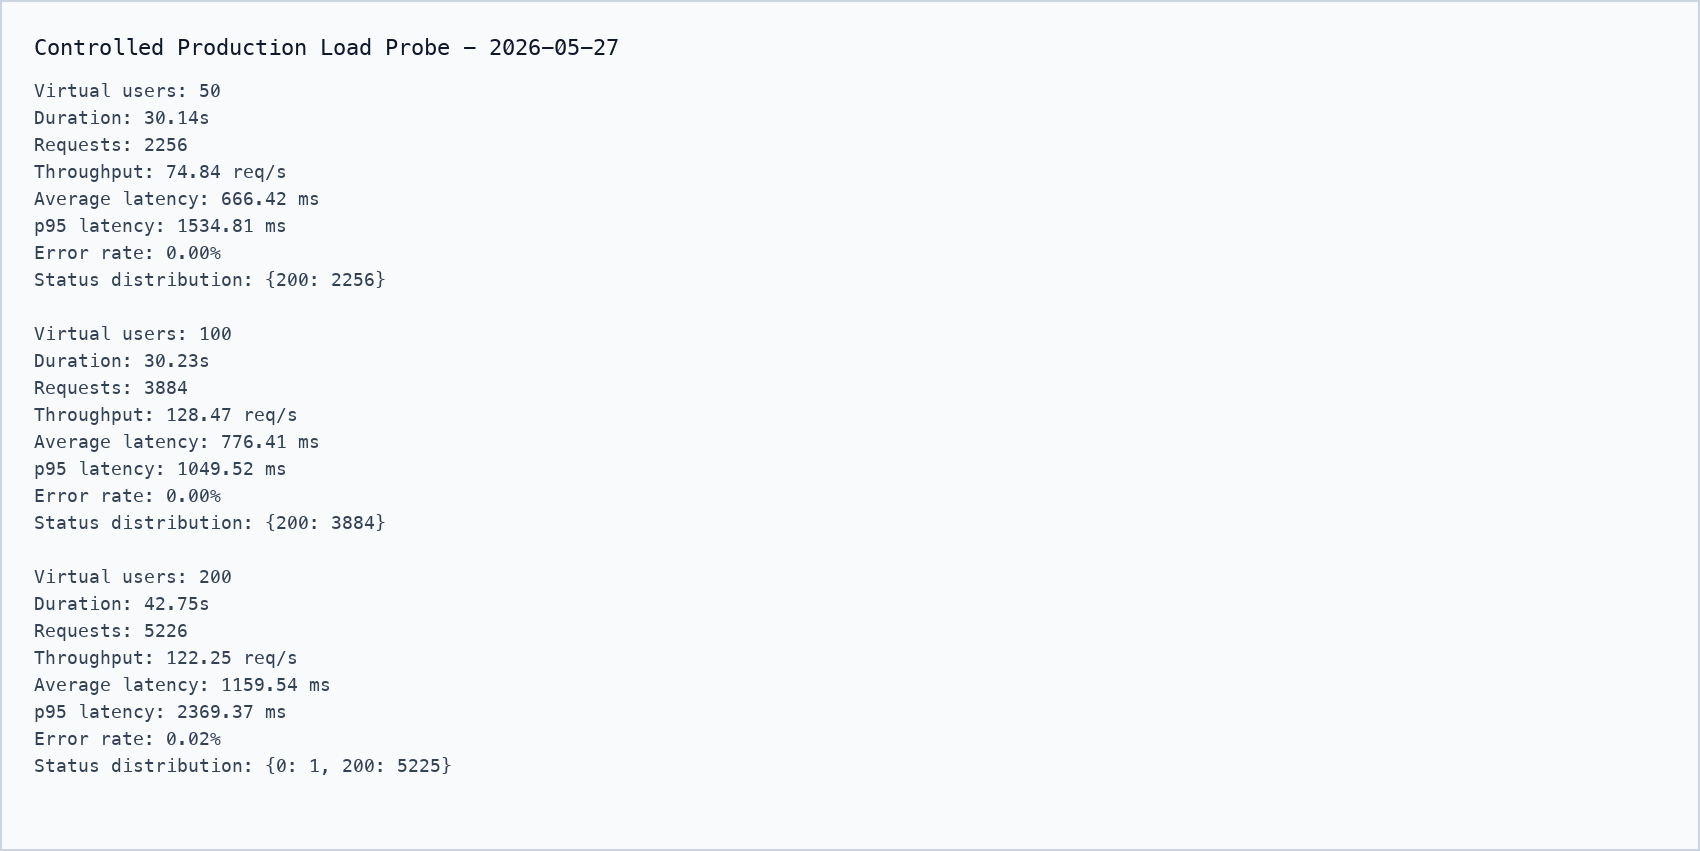
\includegraphics[width=0.95\textwidth]{figures/ch07/test-results/production-load-result.png}
    }{
        \fbox{\parbox[c][5cm][c]{0.9\textwidth}{\centering Thiếu ảnh load test tại \texttt{figures/ch07/test-results/production-load-result.png}}}
    }
    \caption{Kết quả kiểm thử tải có kiểm soát trên production}
    \label{fig:production_load_result}
\end{figure}

\begin{table}[H]
\centering
\small
\renewcommand{\arraystretch}{1.3}
\begin{tabularx}{\textwidth}{|p{1.7cm}|p{2cm}|p{2cm}|p{2cm}|p{2cm}|p{1.8cm}|X|}
\hline
\textbf{Users} & \textbf{Duration} & \textbf{Requests} & \textbf{Throughput} & \textbf{Avg latency} & \textbf{p95} & \textbf{Error/status} \\
\hline
50 & 31.55s & 1205 & 38.19 req/s & 1286.08ms & 2297.99ms & 0.00\%; \texttt{\{200: 1205\}} \\
\hline
100 & 32.03s & 1349 & 42.11 req/s & 2324.92ms & 4191.64ms & 0.00\%; \texttt{\{200: 1349\}} \\
\hline
200 & 32.79s & 1454 & 44.34 req/s & 4347.00ms & 7678.82ms & 0.00\%; \texttt{\{200: 1454\}} \\
\hline
\end{tabularx}
\caption{Kết quả load probe theo bậc trên endpoint tìm kiếm catalog}
\label{tab:production_load_result}
\end{table}

Kết quả cho thấy endpoint tìm kiếm giữ được tính ổn định về mặt lỗi HTTP trong
ba mức tải đã thử: cả 50, 100 và 200 virtual users đều có error rate 0.00\%.
Tuy nhiên latency tăng rõ khi số user đồng thời tăng. Throughput bắt đầu bão hòa
quanh 42--44 request/giây từ mức 100 users, trong khi p95 tăng từ khoảng
2.30 giây ở mức 50 users lên 7.68 giây ở mức 200 users. Vì đây là production
đang phục vụ thật, controlled probe được dừng ở 200 users và không ép tiếp mức
stress cao hơn để tránh tạo tải không cần thiết.

\section{Kết luận kiểm thử}

Thông qua chiến lược kiểm thử phân tầng nghiêm ngặt, dự án đã cung cấp đầy đủ bảo chứng kỹ thuật khẳng định nền tảng Library74 vận hành trơn tru và đạt chuẩn trên cả hai khía cạnh: tính đúng đắn của mã nguồn và độ ổn định trên môi trường thực tế.

Giá trị cốt lõi của quá trình kiểm thử được đúc kết qua các điểm sáng sau:

\begin{itemize}
    \item \textbf{Độ phủ mã nguồn tuyệt đối ở tầng Unit và Contract:} Toàn bộ các phân hệ lõi đều vượt qua rào chắn hồi quy tự động. Cụ thể: Frontend đạt \textbf{62/62} test, Backend đạt \textbf{79/79} test, và AI Service hoàn tất \textbf{72/72} contract test mà không phát sinh bất kỳ ngoại lệ nào.

    \item \textbf{Độ bền bỉ trên môi trường Production:} Tên miền \texttt{library74.uk} vượt qua trọn vẹn \textbf{8/8} kịch bản Smoke Test. Dưới áp lực kiểm thử chịu tải với kịch bản đọc dữ liệu ở ba mốc 50, 100 và 200 người dùng ảo, hệ thống duy trì tỷ lệ lỗi tuyệt đối \textbf{0.00\%}.
    \begin{itemize}
        \item Tại mức 100 người dùng ảo: Thông lượng đạt \textbf{42.11 req/s} với độ trễ \texttt{p95 = 4191.64ms}.
        \item Tại mức 200 người dùng ảo: Thông lượng bão hòa ở mức \textbf{44.34 req/s} với độ trễ \texttt{p95 = 7678.82ms}. Số liệu này chứng minh hệ thống không bị crash khi quá tải, mà tự động chuyển sang cơ chế xếp hàng đợi an toàn.
    \end{itemize}

    \item \textbf{Xóa bỏ tư duy AI hộp đen:} Báo cáo không dừng lại ở việc mô tả tính năng AI một cách trừu tượng, mà định lượng trực tiếp năng lực của mô hình thông qua các độ đo chuẩn học thuật như \texttt{Recall@5}, \texttt{MRR}, \texttt{nDCG@5}, \texttt{Tag F1}, \texttt{Keyword Coverage} và \texttt{Hallucination Guard}. Việc phân hệ AI được đo lường, kiểm soát và có cơ chế Fallback rõ ràng là điểm khác biệt lớn nhất của đồ án.

    \item \textbf{Khả năng giám sát và bảo mật:} Hệ thống được bọc thép bằng các Security Headers tiêu chuẩn, bảo vệ nghiêm ngặt các endpoint nhạy cảm, đồng thời vận hành song song mạng lưới giám sát sức khỏe tự động với Prometheus và cAdvisor.
\end{itemize}

Bên cạnh các thành tựu đạt được, dự án cũng trung thực nhìn nhận các ranh giới kỹ thuật hiện tại nhằm định hình lộ trình nâng cấp:
\begin{enumerate}
    \item \textbf{Đánh giá trích xuất nhãn:} Cần thiết lập một bộ dữ liệu kiểm thử độc lập hoàn toàn, thay vì phụ thuộc một phần vào độ nhất quán của tập nhãn đã được giám tuyển hiện tại.
    \item \textbf{Hệ thống gợi ý:} Cần tích lũy đủ dữ liệu hành vi dài hạn để xây dựng bộ ground truth chuẩn cho hồ sơ người dùng, từ đó mới có thể tiến hành chấm điểm định lượng chính xác.
    \item \textbf{Sức chịu đựng hệ thống:} Kịch bản hiện tại mới dừng ở mức thăm dò có kiểm soát tại 200 người dùng ảo. Hệ thống cần một bài stress test cực hạn để xác định chính xác điểm gãy của phần cứng.
\end{enumerate}

\textbf{Tóm lại,} mặc dù còn những không gian để tối ưu hóa trong dài hạn, các xương sống nghiệp vụ của Library74 đã được kiểm chứng toàn diện bằng bộ test tự động, đánh giá định lượng AI và giám sát trên production. Hệ thống đã sẵn sàng để chuyển giao và đưa vào phục vụ nhu cầu tra cứu học liệu thực tế.

\chapter{Triển khai hệ thống}

\section{Caddy --- Reverse Proxy}

\subsection{Vai trò của Caddy}

Caddy đóng vai trò là reverse proxy trung tâm, tiếp nhận toàn bộ traffic public
từ bên ngoài trên cổng 80/443, tự động cấp HTTPS và định tuyến request đến đúng
dịch vụ nội bộ. Kiến trúc này mang lại hai lợi ích chính: thứ nhất, các cổng
nội bộ của từng container không bị lộ trực tiếp ra internet; thứ hai, client chỉ
cần giao tiếp với một địa chỉ duy nhất là \texttt{https://library74.uk}. Trong
mô hình hiện tại, Nginx vẫn được sử dụng bên trong container frontend để phục vụ
static build của React/Vite, còn Caddy là lớp entrypoint và reverse proxy ở bên
ngoài.

\section{Môi trường sản xuất}

\subsection{Docker Compose sản xuất}

Trong repository hiện tại, cấu hình container được tách theo từng thành phần:
\texttt{LMS\_BE/docker-compose.yml} quản lý PostgreSQL và Kafka cho backend,
còn\\ \texttt{LMS-AI/docker-compose.yml} quản lý RabbitMQ, FastAPI API server và
Celery worker. Frontend và backend có Dockerfile riêng để build image triển
khai. Khi đưa lên server, các thành phần này cần được đặt trong cùng một mạng
triển khai hoặc được cấu hình endpoint rõ ràng thông qua biến môi trường.

Luồng kết nối quan trọng nhất là backend gọi AI qua
\texttt{AI\_GATEWAY\_BASE\_URL}, còn AI service gọi ngược backend qua
\texttt{BACKEND\_WEBHOOK\_URL}. Secret ký callback của hai phía phải khớp nhau:
\texttt{AI\_CALLBACK\_SECRET} ở backend và \texttt{BACKEND\_WEBHOOK\_SECRET}
ở AI service.

Một điểm khác biệt quan trọng so với cấu hình phát triển là giá trị
\path{KAFKA_CFG_ADVERTISED_LISTENERS} được thay đổi từ
\texttt{PLAINTEXT://localhost:9092} thành \texttt{PLAINTEXT://kafka:9092}.
Trong môi trường phát triển, Spring Boot chạy trên máy host nên dùng
\texttt{localhost}; trong môi trường container, Spring Boot nằm trong một
container khác và phải kết nối đến Kafka qua tên service Docker.

\begin{verbatim}
# Hạ tầng Backend
cd LMS_BE && docker compose up -d

# AI Service
cd ../LMS-AI && docker compose up -d --build

# Build image Backend và Frontend
cd ../LMS_BE && docker build -t lms-backend .
cd ../LMS_fe && docker build -t lms-frontend .
\end{verbatim}

\subsection{Quản lý biến môi trường và bảo mật}

Tất cả thông tin nhạy cảm của hệ thống được quản lý thông qua file \texttt{.env}
và không bao giờ được đưa vào mã nguồn (được liệt kê trong \texttt{.gitignore}).
Bảng~\ref{tab:env_vars} liệt kê các nhóm biến môi trường chính.

\begin{table}[h]
\centering
\small
\caption{Các nhóm biến môi trường của hệ thống}
\label{tab:env_vars}
\begin{tabularx}{\textwidth}{|p{2.8cm}|p{6.3cm}|X|}
\hline
\textbf{Nhóm} & \textbf{Biến} & \textbf{Mục đích} \\
\hline
Cơ sở dữ liệu
  & \texttt{DATABASE\_URL} \newline
    \texttt{DATABASE\_USERNAME} \newline
    \texttt{DATABASE\_PASSWORD}
  & Kết nối PostgreSQL \\
\hline
JWT
  & \texttt{EXP\_TOKEN} \newline
    \texttt{EXP\_REFRESH\_TOKEN}
  & Thời hạn Access/Refresh token \\
\hline
OAuth2 Google
  & \texttt{GOOGLE\_CLIENT\_ID} \newline
    \texttt{GOOGLE\_CLIENT\_SECRET} \newline
    \texttt{OAUTH2\_REDIRECT\_URI}
  & Đăng nhập Google \\
\hline
Email
  & \texttt{MAIL\_SENDER\_USERNAME} \newline
    \texttt{MAIL\_SENDER\_PASSWORD}
  & Gửi email qua SMTP \\
\hline
AWS S3
  & \texttt{AWS\_ACCESS\_KEY} \newline
    \texttt{AWS\_SECRET\_KEY}
  & Lưu trữ file (ảnh bìa, tài liệu) \\
\hline
AI Gateway
  & \texttt{AI\_GATEWAY\_BASE\_URL} \newline
    \texttt{AI\_CALLBACK\_SECRET} \newline
    \texttt{AI\_CALLBACK\_MAX\_CLOCK\_} \newline
    \texttt{SKEW\_SECONDS}
  & Backend gọi AI service và xác thực callback \\
\hline
AI Service
  & \texttt{GEMINI\_API\_KEY} \newline
    \texttt{RABBITMQ\_URL} \newline
    \texttt{BACKEND\_WEBHOOK\_URL} \newline
    \texttt{BACKEND\_WEBHOOK\_SECRET}
  & Chạy FastAPI, Celery, Gemini và webhook \\
\hline
PayOS
  & \texttt{CLIENT\_ID\_PAYOS} \newline
    \texttt{API\_KEY\_PAYOS} \newline
    \texttt{CHECKSUM\_KEY\_PAYOS}
  & Tạo và xác thực thanh toán phí phạt \\
\hline
Frontend
  & \texttt{VITE\_API\_BASE\_URL} \newline
    \texttt{VITE\_API\_TIMEOUT}
  & Cấu hình endpoint API và timeout khi build Vite \\
\hline
\end{tabularx}
\end{table}

Khi triển khai lên máy chủ, mỗi thành phần có file môi trường riêng:
\path{LMS_BE.env}, \path{LMS-AI.env} và cấu hình build cho
\texttt{LMS\_fe}. Các file này được tạo từ \texttt{.env.example}, điền giá trị
thực tế trên server và không đưa vào lịch sử git. Với Docker Compose, các biến
được tham chiếu qua \texttt{env\_file} hoặc truyền vào build argument để tránh
nhúng secret vào Docker image.

\subsection{Flyway Migration tự động}

Hệ thống sử dụng Flyway để quản lý phiên bản schema cơ sở dữ liệu. Khi
container Spring Boot khởi động, Flyway tự động thực thi các file migration
chưa được áp dụng theo thứ tự phiên bản trước khi ứng dụng nhận request.
Điều này đảm bảo schema cơ sở dữ liệu luôn đồng bộ với phiên bản ứng dụng
mà không cần can thiệp thủ công.

\begin{verbatim}
library-bootstrap/src/main/resources/db/migration/
+-- V1__create_schema.sql
+-- V8__ai_publication_etl_status.sql
+-- V14__metadata_translations.sql
+-- V20__schema_cleanup_and_ai_indexes.sql
\-- V22__cleanup_ai_metadata_junk.sql
\end{verbatim}

\section{Quy trình khởi tạo hạ tầng ban đầu}

Quy trình thiết lập hệ thống từ đầu trên một máy chủ Linux (Ubuntu Server) trắng bao gồm các bước sau:

\begin{enumerate}
    \item \textbf{Chuẩn bị môi trường máy chủ:} Cài đặt Docker Engine và Docker Compose
          Plugin chính thức từ Docker repository:
\begin{verbatim}
curl -fsSL https://get.docker.com | sh
sudo usermod -aG docker $USER
\end{verbatim}

    \item \textbf{Sao chép mã nguồn:} Tải repository dự án về thư mục quản trị trên máy chủ:
\begin{verbatim}
git clone <repository-url> /opt/library74
cd /opt/library74
\end{verbatim}

    \item \textbf{Cấu hình môi trường vận hành:} Khởi tạo các file biến môi trường bảo mật từ mẫu cấu hình và thiết lập giá trị thực tế (thông số kết nối database, khóa bí mật JWT, API key của bên thứ ba):
\begin{verbatim}
cp LMS_BE/.env.example LMS_BE/.env
cp LMS-AI/.env.example LMS-AI/.env
cp LMS_fe/.env.example LMS_fe/.env
chmod 600 LMS_BE/.env LMS-AI/.env LMS_fe/.env
\end{verbatim}

    \item \textbf{Khởi động hệ thống ban đầu:} Đóng gói và kích hoạt toàn bộ các cụm container dịch vụ:
\begin{verbatim}
cd LMS_BE && docker compose up -d
cd ../LMS-AI && docker compose up -d --build
\end{verbatim}

    \item \textbf{Kiểm tra trạng thái sẵn sàng:} Xác nhận tất cả container vận hành ổn định và đọc log khởi động ban đầu:
\begin{verbatim}
docker compose ps
docker logs -f lms_backend
docker logs -f lms_ai_api
\end{verbatim}
\end{enumerate}

Sau khi khởi động lần đầu, Flyway tự động thực thi các tệp migration của backend. Cụm AI service tự động đồng bộ lược đồ vector, kết nối Message Broker RabbitMQ, tải nạp mô hình Sentence-Transformers về bộ nhớ cache cục bộ và sẵn sàng phục vụ các truy vấn nghiệp vụ.

\section{Hệ thống Tích hợp và Triển khai liên tục (CI/CD Pipeline)}
\label{sec:cicd_pipeline}

\subsection{Đặt vấn đề và mục tiêu thiết kế}

Trong các dự án phần mềm quy mô lớn kết hợp đa nền tảng công nghệ (Java/Spring Boot, Python/FastAPI, React/TypeScript), việc áp dụng quy trình triển khai thủ công (Manual Deployment) bộc lộ nhiều điểm nghẽn nghiêm trọng:
\begin{itemize}[noitemsep]
    \item \textbf{Rủi ro sai sót thao tác (Human Error):} Lập trình viên phải trực tiếp truy cập SSH vào máy chủ sản xuất, tự thực hiện các lệnh kéo mã nguồn và build container, rất dễ nhầm lẫn biến môi trường hoặc xung đột phiên bản.
    \item \textbf{Mã nguồn lỗi lọt vào môi trường Production:} Nếu không có rào chắn kiểm thử tự động bắt buộc trước khi đóng gói, các commit chứa lỗi logic hoặc lỗi hồi quy (regression) có thể làm tê liệt dịch vụ ngay khi đưa lên server.
    \item \textbf{Rủi ro thất thoát dữ liệu:} Quá trình cập nhật phiên bản backend mới thường đi kèm các thay đổi về cấu trúc cơ sở dữ liệu (Flyway migration). Nếu không có cơ chế tự động sao lưu dữ liệu tức thì (snapshot) ngay trước thời điểm deploy, việc khôi phục dữ liệu khi xảy ra lỗi là vô cùng phức tạp.
    \item \textbf{Thời gian ngưng trệ dịch vụ (Downtime) kéo dài:} Việc biên dịch ứng dụng và build Docker image trực tiếp trên máy chủ gây quá tải CPU/RAM, ảnh hưởng trực tiếp đến người dùng đang hoạt động.
\end{itemize}

Nhằm khắc phục toàn diện các vấn đề trên, hệ thống CI/CD của dự án Library74 được thiết kế dựa trên nền tảng GitHub Actions với 4 mục tiêu cốt lõi:
\begin{enumerate}[noitemsep]
    \item \textbf{Tự động hóa toàn diện 100\% (End-to-End Automation):} Mọi thay đổi mã nguồn sau khi được gộp (merge) vào nhánh chính \texttt{main} đều tự động kích hoạt kiểm thử, đóng gói và triển khai lên máy chủ mà không cần can thiệp thủ công.
    \item \textbf{Kiến trúc Monorepo phân tách theo module (Path-filtered Pipeline):} Bộ lọc đường dẫn thay đổi giúp tách biệt hoàn toàn pipeline của ba phân hệ độc lập (\texttt{LMS\_BE}, \texttt{LMS\_FE}, \texttt{LMS\_AI}), giúp tiết kiệm tài nguyên và rút ngắn tối đa thời gian phát hành.
    \item \textbf{An toàn dữ liệu tuyệt đối (Zero Data Loss):} Luôn tự động chụp bản sao lưu cơ sở dữ liệu nhị phân (Database Snapshot) trước khi bất kỳ phiên bản backend mới nào được khởi chạy.
    \item \textbf{Kiểm tra sức khỏe dịch vụ tự động (Post-deployment Health Check):} Tự động thăm dò trạng thái sẵn sàng của container trước khi chính thức đánh dấu quá trình triển khai thành công.
\end{enumerate}

\subsection{Kiến trúc tổng thể và luồng hoạt động}

Kiến trúc luồng hoạt động của hệ thống CI/CD được minh họa chi tiết trong Hình~\ref{fig:cicd_flow}. Quy trình được chia thành bốn giai đoạn kế tiếp nhau với sự phân định rạch ròi về môi trường thực thi:
\begin{enumerate}
    \item \textbf{Giai đoạn Kích hoạt (Trigger):} Lập trình viên đẩy commit hoặc hoàn tất Pull Request sáp nhập vào nhánh \texttt{main}. Bộ lọc đường dẫn (\textit{Path Filter}) phân tích các tệp tin sửa đổi để xác định phân hệ bị ảnh hưởng.
    \item \textbf{Giai đoạn Tích hợp liên tục (CI):} Khởi chạy máy ảo độc lập trên GitHub Actions Runner. Từng phân hệ thực hiện khôi phục bộ nhớ đệm (cache), chạy kiểm thử tự động và biên dịch thử nghiệm.
    \item \textbf{Cổng kiểm soát chất lượng (Quality Gate):} Toàn bộ các bài kiểm tra phải đạt trạng thái \texttt{success}. Nếu có bất kỳ kiểm thử nào thất bại, pipeline lập tức dừng lại, gửi thông báo cảnh báo và từ chối tiến hành triển khai.
    \item \textbf{Giai đoạn Triển khai liên tục (CD):} Máy ảo GitHub kết nối tới máy chủ sản xuất (Production VPS) thông qua giao thức SSH với khóa bảo mật riêng biệt, đồng bộ mã nguồn, thực hiện snapshot dữ liệu, biên dịch container và kiểm tra phản hồi của dịch vụ.
\end{enumerate}
\begin{figure}[H]
\centering
\begin{tikzpicture}[
    scale=0.65, transform shape,
    % Styles
    startstop/.style={rectangle, draw=blue!80!black, fill=blue!10, rounded corners=4pt, text width=4.8cm, minimum height=0.9cm, align=center, font=\small\bfseries},
    cibox/.style={rectangle, draw=teal!80!black, fill=teal!8, rounded corners=4pt, text width=3.4cm, minimum height=1.35cm, align=center, font=\footnotesize},
    cdbox/.style={rectangle, draw=orange!90!black, fill=orange!8, rounded corners=4pt, text width=4.8cm, minimum height=0.85cm, align=center, font=\footnotesize},
    decision/.style={diamond, draw=purple!80!black, fill=purple!8, aspect=2.2, inner sep=2pt, align=center, font=\scriptsize\bfseries},
    respass/.style={rectangle, draw=green!60!black, fill=green!15, rounded corners=4pt, text width=3.8cm, minimum height=0.85cm, align=center, font=\footnotesize\bfseries},
    resfail/.style={rectangle, draw=red!70!black, fill=red!12, rounded corners=4pt, text width=3.8cm, minimum height=0.85cm, align=center, font=\footnotesize\bfseries},
    cigroup/.style={draw=teal!70!black, dashed, rounded corners=6pt, line width=0.9pt, inner sep=10pt},
    cdgroup/.style={draw=orange!80!black, dashed, rounded corners=6pt, line width=0.9pt, inner sep=10pt},
    arrow/.style={-{Stealth[scale=0.9]}, thick, draw=gray!80!black},
    lbl/.style={font=\scriptsize\itshape, fill=white, inner sep=1.5pt}
]

% 1. DEVELOPER
\node[startstop] (dev) at (0, 0) {Developer Push / Merge\\{\normalfont\scriptsize Nhánh chính \texttt{main} trên GitHub}};

% 2. PATH FILTER
\node[decision, below=0.6cm of dev] (filter) {Bộ lọc đường dẫn\\{\normalfont\scriptsize (Path-filtered Trigger)}};

% 3. CI NODES
\node[cibox, below=1.3cm of filter] (ci_fe) {
    \textbf{Frontend CI}\\[2pt]
    \scriptsize Node.js 20 \& NPM Cache\\
    Jest Unit Tests\\
    Vite Production Build\\
    Build thử Docker Nginx
};

\node[cibox, left=0.7cm of ci_fe] (ci_be) {
    \textbf{Backend CI}\\[2pt]
    \scriptsize JDK 21 \& Maven Cache\\
    Unit \& Integration Tests\\
    Build thử Docker Backend
};

\node[cibox, right=0.7cm of ci_fe] (ci_ai) {
    \textbf{AI Service CI}\\[2pt]
    \scriptsize Python 3.10 \& Pip Cache\\
    Compileall syntax check\\
    Pytest Logic Tests\\
    (Bỏ build Docker nặng)
};

% CI Group
\node[cigroup, fit=(ci_be) (ci_fe) (ci_ai)] (ci_group) {};
\node[font=\footnotesize\bfseries, text=teal!90!black, fill=white, inner sep=2pt, anchor=south] at ([yshift=8pt]ci_be.north) {Giai đoạn 1: Tích hợp liên tục (CI)};

% 4. QUALITY GATE
\node[decision, below=1.2cm of ci_fe] (gate) {Quality Gate\\{\normalfont\scriptsize CI thành công trên nhánh \texttt{main}?}};

% 5. CD NODES (Production VPS)
\node[cdbox, below=1.4cm of gate] (ssh) {
    \textbf{1. Xác thực SSH an toàn}\\
    \scriptsize Private Key \texttt{ed25519} + Known Hosts
};

\node[cdbox, below=0.45cm of ssh] (pull) {
    \textbf{2. Đồng bộ mã nguồn an toàn}\\
    \scriptsize \texttt{git pull --ff-only origin main}
};

\node[cdbox, below=0.45cm of pull] (dump) {
    \textbf{3. Sao lưu Database tự động}\\
    \scriptsize Snapshot \texttt{library-*.dump} nén nhị phân
};

\node[cdbox, below=0.45cm of dump] (rebuild) {
    \textbf{4. Cập nhật container độc lập}\\
    \scriptsize \texttt{docker compose up -d --build <service>}
};

\node[cdbox, below=0.45cm of rebuild, draw=purple!80!black, fill=purple!8] (health) {
    \textbf{5. Vòng lặp Polling Health Check (36 lần $\times$ 5s)}\\
    \scriptsize Backend Actuator / AI FastAPI / Nginx \& Public Domain
};

\node[respass, below left=0.7cm and 0.2cm of health] (success) {
    Triển khai THÀNH CÔNG\\
    {\normalfont\scriptsize Dịch vụ sẵn sàng phục vụ}
};

\node[resfail, below right=0.7cm and 0.2cm of health] (fail) {
    Triển khai THẤT BẠI\\
    {\normalfont\scriptsize Giữ snapshot DB \& gửi cảnh báo}
};

% CD Group
\node[cdgroup, fit=(ssh) (pull) (dump) (rebuild) (health) (success) (fail)] (cd_group) {};
\node[font=\footnotesize\bfseries, text=orange!90!black, fill=white, inner sep=2pt, anchor=south west] at ([xshift=6pt, yshift=3pt]cd_group.north west) {Giai đoạn 2: Triển khai liên tục (CD trên VPS)};

% CONNECTING ARROWS
\draw[arrow] (dev) -- (filter);
\draw[arrow] (filter) -| node[lbl, pos=0.45] {\texttt{LMS\_BE/**}} (ci_be);
\draw[arrow] (filter) -- node[lbl, right=2pt, pos=0.35] {\texttt{LMS\_FE/**}} (ci_fe);
\draw[arrow] (filter) -| node[lbl, pos=0.45] {\texttt{LMS\_AI/**}} (ci_ai);

\draw[arrow] (ci_be) |- (gate);
\draw[arrow] (ci_fe) -- (gate);
\draw[arrow] (ci_ai) |- (gate);

\draw[arrow] (gate) -- node[lbl, right=2pt, pos=0.4] {Đạt (Pass)} (ssh);
\draw[arrow] (ssh) -- (pull);
\draw[arrow] (pull) -- (dump);
\draw[arrow] (dump) -- (rebuild);
\draw[arrow] (rebuild) -- (health);

\draw[arrow] (health) -| node[lbl, near start] {HTTP 200 / UP} (success);
\draw[arrow] (health) -| node[lbl, near start] {Lỗi / Hết giờ} (fail);

\end{tikzpicture}
\caption{Kiến trúc tổng thể luồng CI/CD trong hệ thống Library74}
\label{fig:cicd_flow}
\end{figure}

\subsection{Chi tiết giai đoạn Tích hợp liên tục (CI)}

Giai đoạn CI được thực thi trên môi trường máy ảo Ubuntu sạch của GitHub (\textit{GitHub-hosted Runner}). Bảng~\ref{tab:ci_workflows} tổng hợp các workflow CI tương ứng với từng thành phần kiến trúc.

\begin{table}[htbp]
\centering
\small
\caption{Chi tiết các workflow Tích hợp liên tục (CI)}
\label{tab:ci_workflows}
\renewcommand{\arraystretch}{1.3}
\begin{tabularx}{\textwidth}{|p{2.6cm}|p{3.3cm}|X|p{1.8cm}|}
\hline
\textbf{Thành phần} & \textbf{Tệp cấu hình} & \textbf{Nhiệm vụ chính} & \textbf{Thời gian} \\
\hline
\textbf{Backend CI} &
\texttt{backend-ci.yml} \newline
{\scriptsize \path{.github/workflows/}} &
- Cấu hình OpenJDK 21 Temurin kèm cache Maven. \newline
- Thực thi toàn bộ Unit \& Integration Test suite. \newline
- Build thử nghiệm Docker Image Backend nhằm xác thực Dockerfile multi-stage. &
$\sim$1--2 phút \\
\hline
\textbf{Frontend CI} &
\texttt{frontend-ci.yml} \newline
{\scriptsize \path{.github/workflows/}} &
- Cấu hình Node.js 20 kèm cache NPM package. \newline
- Cài đặt sạch các gói phụ thuộc (\texttt{npm ci}). \newline
- Chạy toàn bộ Unit Test giao diện bằng Jest. \newline
- Biên dịch gói tĩnh Vite (\texttt{npm run build}). \newline
- Build thử nghiệm Docker Image Nginx đóng gói web. &
$\sim$1--2 phút \\
\hline
\textbf{AI Service CI} &
\texttt{ai-ci.yml} \newline
{\scriptsize \path{.github/workflows/}} &
- Cấu hình Python 3.10 kèm cache Pip wheel. \newline
- Biên dịch kiểm tra toàn bộ cú pháp (\texttt{compileall}). \newline
- Thực thi bộ test logic và hợp đồng bằng Pytest. &
$\sim$1--2 phút \\
\hline
\end{tabularx}
\end{table}

\noindent \textbf{Chiến lược tối ưu hóa đặc thù cho phân hệ AI CI:}
Trong quá trình thiết kế pipeline, phân hệ AI Service sử dụng các thư viện tính toán khoa học và học sâu rất nặng như \texttt{torch} ($\sim$1GB), \texttt{sentence-transformers}, \texttt{scipy}. Nếu áp dụng bước \texttt{docker build} trên GitHub-hosted Runner, máy ảo sẽ phải tải lại toàn bộ PyTorch và model weights từ đầu mà không có lớp cache cục bộ, dẫn đến thời gian thực thi CI kéo dài từ 12 đến 15 phút, gây lãng phí nghiêm trọng quota tính giờ của GitHub Actions.

Để tối ưu, nhóm phát triển đã đưa ra quyết định kiến trúc: \textit{Tách biệt hoàn toàn việc kiểm thử logic và đóng gói container đối với AI Service}. Phân hệ AI CI trên GitHub Runner chỉ tập trung biên dịch cú pháp mã nguồn và chạy Pytest với môi trường Python chuẩn. Việc đóng gói Docker image được chuyển giao hoàn toàn cho máy chủ VPS trong giai đoạn CD. Tại VPS, Docker Daemon đã lưu trữ sẵn các layer cơ sở của PyTorch và thư viện AI trong bộ nhớ đệm cục bộ, do đó quá trình build lại image khi có cập nhật mã nguồn mới chỉ tiêu tốn từ 3 đến 5 giây.

\subsection{Chi tiết giai đoạn Triển khai liên tục (CD)}

Giai đoạn Triển khai liên tục (CD) được kích hoạt tự động theo cơ chế liên kết sự kiện \texttt{workflow\_run}, với điều kiện bắt buộc là workflow CI tương ứng đã hoàn thành thành công (\texttt{conclusion == 'success'}) trên nhánh \texttt{main}, hoặc có thể được người quản trị kích hoạt thủ công thông qua sự kiện \texttt{workflow\_dispatch}.

Quá trình CD trên máy chủ Production tuân thủ nghiêm ngặt quy trình an toàn 6 bước sau:

\begin{enumerate}
    \item \textbf{Xác thực bảo mật SSH không mật khẩu (Zero Password Authentication):}
    Pipeline sử dụng Private Key chuẩn mã hóa hiện đại \texttt{ed25519} được lưu trữ an toàn trong GitHub Secrets (\texttt{DEPLOY\_SSH\_KEY}). Trước khi mở kết nối, GitHub Runner tiến hành đối soát dấu vân tay máy chủ thông qua biến \texttt{DEPLOY\_KNOWN\_HOSTS}, loại trừ hoàn toàn nguy cơ bị tấn công giả mạo máy chủ (Man-in-the-Middle).

    \item \textbf{Đồng bộ mã nguồn an toàn (Fast-forward Synchronization):}
    Lệnh kéo mã nguồn sử dụng cờ \texttt{--ff-only} để đảm bảo lịch sử git trên máy chủ luôn là một đường thẳng khớp chính xác với commit đã qua kiểm thử trên nhánh \texttt{main}:
\begin{verbatim}
cd /opt/library74
git pull --ff-only origin main
\end{verbatim}
    Cơ chế này ngăn chặn tuyệt đối tình trạng máy chủ tự động tạo merge commit bất thường ngoài tầm kiểm soát khi môi trường thực thi bị can thiệp.

    \item \textbf{Kiểm tra tính hợp lệ của cấu hình triển khai:}
    Trước khi thay đổi bất kỳ trạng thái nào của dịch vụ đang chạy, Docker Compose thực hiện kiểm tra cú pháp và tham chiếu biến môi trường:
\begin{verbatim}
docker compose --env-file .env.prod \
  -f docker-compose.prod.yml config >/dev/null
\end{verbatim}

    \item \textbf{Bảo vệ dữ liệu tự động (Pre-deployment Database Snapshot):}
    Đối với phân hệ Backend CD, nhằm phòng tránh rủi ro migration thất bại gây hỏng dữ liệu, hệ thống tự động kích hoạt container sao lưu cơ sở dữ liệu:
\begin{verbatim}
docker compose --env-file .env.prod -f docker-compose.prod.yml \
  --profile backup run --rm postgres-backup
\end{verbatim}
    Tác vụ này tạo ra bản chụp cơ sở dữ liệu nhị phân nén dạng \path{library-YYYYMMDD-HHMMSS.dump} lưu trữ trong thư mục \path{backups/} trên máy chủ trước khi phiên bản backend mới khởi chạy và chạy migration.

    \item \textbf{Cập nhật dịch vụ độc lập không gián đoạn (Zero Interruption):}
    Hệ thống áp dụng cơ chế triển khai theo từng container chuyên biệt, tránh việc restart toàn bộ hệ thống gây gián đoạn:
    \begin{itemize}[noitemsep]
        \item Backend: \texttt{docker compose ... up -d --build backend}
        \item AI Service: \texttt{docker compose ... up -d --build ai-api ai-worker}
        \item Frontend: \texttt{docker compose ... up -d --build frontend}
    \end{itemize}
    Các dịch vụ hạ tầng nền tảng như PostgreSQL, Kafka, RabbitMQ, Caddy Reverse Proxy vẫn duy trì kết nối liên tục 100\% mà không bị ngắt quãng.

    \item \textbf{Kiểm tra sức khỏe dịch vụ sau triển khai (Post-deployment Health Check):}
    Để khẳng định container mới không chỉ ``đang chạy'' (running) mà đã thực sự sẵn sàng phục vụ yêu cầu của người dùng, script CD thực hiện vòng lặp thăm dò (polling) tối đa 36 lần, mỗi lần cách nhau 5 giây (thời gian chờ tối đa 3 phút):
    \begin{itemize}[noitemsep]
        \item \textbf{Backend:} Truy vấn actuator health endpoint nội bộ:
\begin{verbatim}
docker compose exec -T backend wget -qO- \ 
  http://127.0.0.1:8080/actuator/health | grep -q UP
\end{verbatim}
        \item \textbf{AI Service:} Truy vấn endpoint kiểm tra trạng thái của FastAPI:
\begin{verbatim}
docker compose exec -T ai-api \
curl -fsS http://127.0.0.1:8001/health
\end{verbatim}
        \item \textbf{Frontend:} Kiểm tra đồng thời phản hồi HTTP của Nginx nội bộ và domain công khai:
\begin{verbatim}
docker compose exec -T frontend wget -qO- http://127.0.0.1/ \ 
  >/dev/null && curl -fsS https://library74.uk/ >/dev/null
\end{verbatim}
    \end{itemize}
    Nếu sau 36 lần thăm dò mà dịch vụ không phản hồi mã trạng thái thành công, pipeline lập tức báo lỗi \textit{Deployment Failed} và gửi thông báo cho đội ngũ quản trị để kịp thời xử lý.
\end{enumerate}

\subsection{Quản lý bảo mật và phân tách cấu hình bí mật}

Hệ thống tuân thủ nguyên tắc đặc quyền tối thiểu (Principle of Least Privilege) bằng cách phân tách cấu hình thành hai lớp bảo mật:
\begin{itemize}
    \item \textbf{Biến môi trường nghiệp vụ (\texttt{.env.prod}):} Được lưu trữ cố định trên máy chủ sản xuất với phân quyền nghiêm ngặt (\texttt{chmod 600}, chỉ user quản trị hệ thống mới có quyền đọc/ghi). Các khóa nhạy cảm bao gồm mật khẩu database, S3 secret key, API key PayOS và token kết nối không bao giờ được đưa vào mã nguồn hay lưu trên kho lưu trữ git.
    \item \textbf{Biến môi trường triển khai (GitHub Repository Secrets):} Chỉ chứa các thông số định danh cần thiết để phục vụ quá trình kết nối và vận hành tự động: \texttt{DEPLOY\_HOST}, \texttt{DEPLOY\_PORT}, \texttt{DEPLOY\_USER}, \texttt{DEPLOY\_PATH}, khóa bảo mật \texttt{DEPLOY\_SSH\_KEY} và chuỗi định danh \texttt{DEPLOY\_KNOWN\_HOSTS}.
\end{itemize}

\subsection{Đánh giá định lượng hiệu quả hệ thống}

Việc đưa hệ thống CI/CD vào vận hành chính thức đã nâng cao rõ rệt độ tin cậy, an toàn và tốc độ phát hành của dự án. Bảng~\ref{tab:cicd_evaluation} so sánh định lượng các chỉ số vận hành then chốt trước và sau khi triển khai giải pháp CI/CD.

\begin{table}[htbp]
\centering
\small
\caption{Đánh giá hiệu quả vận hành trước và sau khi áp dụng CI/CD}
\label{tab:cicd_evaluation}
\renewcommand{\arraystretch}{1.3}
\begin{tabularx}{\textwidth}{|p{3.5cm}|p{4.8cm}|X|}
\hline
\textbf{Tiêu chí đánh giá} & \textbf{Quy trình thủ công (Trước)} & \textbf{Hệ thống CI/CD (Sau)} \\
\hline
\textbf{Thời gian phát hành} &
15--30 phút (đăng nhập SSH, gõ lệnh thủ công từng dịch vụ). &
\textbf{Dưới 3 phút} (tự động hóa 100\% từ khi push code). \\
\hline
\textbf{Kiểm định chất lượng mã nguồn} &
Phụ thuộc sự cẩn thận của lập trình viên, dễ bỏ sót test. &
\textbf{100\% tự động vượt qua test suite} trước khi được phép triển khai. \\
\hline
\textbf{An toàn dữ liệu cơ sở dữ liệu} &
Thực hiện thủ công, dễ bị lãng quên trước khi cập nhật. &
\textbf{Tự động chụp snapshot nhị phân} trước mỗi lần deploy Backend. \\
\hline
\textbf{Mức độ gián đoạn dịch vụ (Downtime)} &
Downtime kéo dài do máy chủ bị chiếm dụng tài nguyên để build image. &
\textbf{Tối thiểu hóa downtime} nhờ cập nhật tách biệt theo container. \\
\hline
\textbf{Phát hiện lỗi phát hành} &
Phát hiện muộn thông qua phản ánh của người dùng hoặc kiểm tra thủ công. &
\textbf{Hệ thống Polling Health Check} tự động bắt lỗi ngay trong 3 phút đầu. \\
\hline
\end{tabularx}
\end{table}

\noindent Kết quả cho thấy hệ thống CI/CD không chỉ loại bỏ hoàn toàn các thao tác thủ công rủi ro mà còn thiết lập một quy trình chuyển giao phần mềm tiêu chuẩn, an toàn và có khả năng phục hồi cao theo đúng chuẩn mực công nghiệp trong phát triển phần mềm hiện đại.

\section{Hạ tầng mạng: Domain và HTTPS}

\subsection{Tên miền (Domain)}

Trong bản triển khai demo, hệ thống sử dụng tên miền \texttt{library74.uk} để
người dùng truy cập bằng một địa chỉ ổn định thay vì ghi nhớ IP hoặc cổng dịch
vụ. DNS của domain được quản lý qua Cloudflare và trỏ về Google Cloud VPS. Tại
VPS, Caddy nhận request HTTPS, tự động xử lý chứng chỉ TLS và định tuyến request
đến frontend, backend API hoặc WebSocket theo path tương ứng.

Luồng kết nối sau khi đi vào backend tiếp tục được phân tách theo trách nhiệm:
Spring Boot xử lý nghiệp vụ chính và kết nối PostgreSQL/Kafka; backend gọi AI
Service qua \path{AI_GATEWAY_BASE_URL}; AI worker xử lý PDF bất đồng bộ qua
RabbitMQ và callback kết quả về backend bằng chữ ký HMAC. Các tích hợp ngoài
như S3-compatible storage, PayOS, Gmail SMTP, Google OAuth2 và Gemini API được
kết nối từ backend hoặc AI worker theo đúng vai trò của từng dịch vụ.

\begin{figure}[h]
    \centering
    \includegraphics[width=0.95\textwidth]{figures/ch09/dns_flow.png}
    \caption{Luồng kết nối từ tên miền Library74 đến hệ thống production}
    \label{fig:dns_flow}
\end{figure}

\subsection{Tổng chi phí vận hành}

Bảng~\ref{tab:hosting_cost} được điều chỉnh theo chi phí triển khai hiện tại.
Tên miền \texttt{library74.uk} được mua theo năm, còn máy chủ demo đang chạy
trên Google Cloud Platform với cấu hình ước tính khoảng 92 USD/năm. Tại thời
điểm triển khai demo, GCP đang có ưu đãi miễn phí 3 tháng nên chi phí thực trả
ban đầu thấp hơn chi phí vận hành ổn định về sau.

\begin{table}[h]
\centering
\small
\caption{Chi phí vận hành hệ thống trong cấu hình demo}
\label{tab:hosting_cost}
\begin{tabularx}{\textwidth}{|p{3.5cm}|p{3.3cm}|p{2cm}|X|}
\hline
\textbf{Thành phần} & \textbf{Chi phí} & \textbf{Chu kỳ} & \textbf{Ghi chú} \\
\hline
Tên miền \texttt{library74.uk} & 5,3 USD & Năm & Khoản bắt buộc để giữ địa chỉ public của demo. \\
\hline
SSL/HTTPS & Miễn phí & 90 ngày hoặc tự động & Let's Encrypt hoặc chứng chỉ tự động từ reverse proxy/nhà cung cấp. \\
\hline
Google Cloud Platform & 92 USD & Năm & Chi phí theo cấu hình máy chủ demo; hiện đang được miễn phí 3 tháng đầu. \\
\hline
Lưu trữ file & Theo mức sử dụng & Tháng & Ảnh bìa/PDF dùng object storage hoặc cấu hình tương đương; chi phí phụ thuộc dung lượng thực tế. \\
\hline
API ngoài & Miễn phí trong phạm vi demo & Tháng & Google OAuth, Gmail SMTP, PayOS sandbox/quota demo và Gemini quota thử nghiệm. \\
\hline
\textbf{Tổng cố định ước tính} & \textbf{97,3 USD} & \textbf{Năm} & Chưa tính ưu đãi miễn phí 3 tháng GCP và chi phí phát sinh theo dung lượng/request thực tế. \\
\hline
\end{tabularx}
\end{table}

\noindent Như vậy, sau giai đoạn miễn phí ban đầu, chi phí cố định tối thiểu của
hệ thống chủ yếu gồm tên miền và máy chủ GCP, khoảng 97,3 USD/năm theo cấu hình
demo. Khi triển khai production thật, các thông số cần được cập nhật lại theo dung lượng PDF,
số lượt truy vấn AI và chính sách giá của nhà cung cấp tại thời điểm vận hành.

% --- BẮT ĐẦU PHẦN TỔNG KẾT ---

\chapter{Tổng kết}

Dự án ``Hệ thống Quản lý Thư viện Trực tuyến tích hợp AI'' (Library74) được định hình và phát triển với tầm nhìn chuyển đổi số quy trình vận hành thư viện. Vượt qua giới hạn của một phần mềm quản lý thông thường, dự án đã hiện thực hóa một kiến trúc phân tán bao gồm ba phân lớp lõi: Frontend, Backend và AI Service.

\begin{figure}[H]
    \centering
    \includegraphics[width=0.22\textwidth]{figures/ch09/logo.png}
    \caption{Nhận diện thương hiệu của nền tảng Library74}
    \label{fig:library74_logo_conclusion}
\end{figure}

\section{Tổng hợp kết quả hiện thực}

Đóng góp cốt lõi của đồ án không nằm ở việc xây dựng các module đơn lẻ, mà ở khả năng liên kết các phân hệ thành những luồng dữ liệu và luồng nghiệp vụ khép kín, hoạt động ổn định trên môi trường triển khai thực tế.

\subsection{Phân lớp Frontend}

Thay vì liệt kê các màn hình rời rạc, lớp giao diện được định hình theo nhóm người dùng để tối ưu hóa trải nghiệm tương tác:

\begin{itemize}
    \item \textbf{Trang công cộng:} Triển khai cơ chế kết xuất trang tĩnh và kết xuất phía máy chủ cho trang chủ, luồng tìm kiếm, đăng nhập OAuth2 và khôi phục mật khẩu. Điều này giúp giảm thiểu rào cản tiếp cận, tối ưu hóa công cụ tìm kiếm (SEO) và cung cấp điểm chạm đầu tiên mượt mà cho độc giả.
    \item \textbf{Khu vực độc giả:} Xây dựng dashboard cá nhân hóa, quản lý vòng đời phiếu mượn, thanh toán mã QR, hệ thống Wishlist, Rating và thông báo thời gian thực. Các tính năng này giao quyền chủ động cho độc giả trong việc tự phục vụ và theo dõi tài nguyên học tập cá nhân.
    \item \textbf{Khu vực vận hành:} Thiết kế giao diện quản lý vòng đời ấn phẩm, kiểm soát hàng chờ, xử lý phạt và mất sách cùng dashboard điều hành. Phân hệ này hỗ trợ số hóa nghiệp vụ thủ công, gom cụm các thao tác vận hành vào một không gian làm việc duy nhất.
    \item \textbf{Khu vực quản trị:} Cung cấp công cụ cấu hình chính sách thư viện, quản trị định danh, phân quyền và giám sát hệ thống qua Audit Log, đảm bảo tính toàn vẹn, bảo mật và khả năng kiểm toán hệ thống minh bạch.
    \item \textbf{Tối ưu nền tảng:} Áp dụng quản lý trạng thái linh hoạt, hỗ trợ đa ngôn ngữ, hệ thống giao diện sáng tối, Route Guard và luồng Refresh Token ngầm để duy trì sự liền mạch trong các phiên làm việc kéo dài.
\end{itemize}

\subsection{Phân lớp Backend}

Máy chủ trung tâm đảm nhiệm vai trò kiểm soát toàn vẹn dữ liệu và điều phối các luồng xử lý phức tạp:

\begin{itemize}
    \item \textbf{Quản trị định danh:} Sử dụng JWT, cơ chế xoay vòng token, xác thực email, Google OAuth2 và kiểm soát quyền truy cập dựa trên vai trò để tạo lập rào chắn bảo mật vững chắc cho toàn bộ API.
    \item \textbf{Quản lý tài nguyên:} Chuẩn hóa lược đồ cho ấn phẩm, tác giả, danh mục và tích hợp Storage Port lưu trữ file số an toàn, định hình nguồn dữ liệu chuẩn xác cho tài nguyên thư viện.
    \item \textbf{Luồng mượn trả:} Xử lý giao dịch mượn trả tuân thủ nguyên tắc ACID, quản lý hàng chờ đặt trước, xử lý ngoại lệ trễ hạn và mất sách, giải quyết bài toán cốt lõi của nghiệp vụ thư viện truyền thống.
    \item \textbf{Thanh toán và sự kiện:} Tích hợp cổng PayOS qua Webhook, xây dựng kiến trúc hướng sự kiện với Kafka cho thông báo và Scheduler định kỳ nhắc hạn nhằm thúc đẩy tự động hóa và giảm độ trễ phản hồi.
    \item \textbf{Hạ tầng và hệ thống:} Quản lý lược đồ dữ liệu với Flyway, xử lý lỗi tập trung và tích hợp AI Gateway với cơ chế bảo mật chữ ký HMAC, giúp hệ thống dễ dàng mở rộng và bảo trì trong dài hạn.
\end{itemize}

\subsection{Phân lớp AI Service}

Phân hệ trí tuệ nhân tạo được thiết kế như một dịch vụ độc lập nhằm tránh gây áp lực lên luồng xử lý đồng bộ của hệ thống chính:

\begin{itemize}
    \item \textbf{Luồng xử lý dữ liệu PDF:} Tự động trích xuất ngữ nghĩa bằng PyMuPDF, làm sạch nhiễu, phân mảnh văn bản và tối ưu tính toán để bỏ qua các file trùng lặp, giúp chuyển đổi dữ liệu phi cấu trúc thành định dạng tiêu chuẩn.
    \item \textbf{Mô hình nhúng vector:} Khởi tạo vector đa chiều với SentenceTransformer chuẩn hóa tiếng Việt, lưu trữ và truy xuất thông qua pgvector trên PostgreSQL để giải quyết bài toán tìm kiếm ngữ nghĩa theo khoảng cách.
    \item \textbf{Làm giàu siêu dữ liệu:} Điều phối mô hình ngôn ngữ sinh tóm tắt, trích xuất nhãn đa ngữ và giới hạn tình trạng ảo giác qua cơ chế ép định dạng JSON, giúp giảm thiểu đáng kể công việc nhập liệu thủ công của thủ thư.
    \item \textbf{Hệ thống gợi ý:} Áp dụng thuật toán kết hợp giữa lọc cộng tác, phân tích nội dung và cơ chế đề xuất theo xu hướng cho người dùng mới, từng bước cá nhân hóa trải nghiệm khám phá tri thức.
    \item \textbf{Kiến trúc bất đồng bộ:} Tách biệt xử lý bằng FastAPI và Celery Worker qua RabbitMQ, giao tiếp an toàn với Backend qua mã hóa HMAC để ngăn chặn hiện tượng nghẽn cổ chai khi xử lý tác vụ AI nặng.
\end{itemize}

\subsection{Kiểm thử và Đảm bảo chất lượng}

Để minh chứng cho tính ổn định, hệ thống đã trải qua các kịch bản kiểm thử phân tầng với kết quả khả quan:

\begin{itemize}
    \item \textbf{Kiểm thử Frontend:} Vượt qua 62/62 kịch bản Unit Test và Component Test cho logic giao diện, quản lý trạng thái và tính hợp lệ của biểu mẫu, đảm bảo tính chống chịu lỗi phía người dùng.
    \item \textbf{Kiểm thử Backend:} Vượt qua 79/79 kịch bản Integration Test tập trung vào logic nghiệp vụ, luồng giao dịch cơ sở dữ liệu và bảo mật API. Luồng cập nhật dữ liệu hoạt động nhất quán, không xảy ra hiện tượng bế tắc.
    \item \textbf{Đánh giá AI Service:} Hoàn tất 72/72 Contract Test cho luồng xử lý tự động. Việc đo lường trên tập dữ liệu chuẩn ghi nhận nDCG@5 đạt 0.907, Recall@5 đạt 87.5\% và độ trễ p95 ở mức 540ms.
    \item \textbf{Vận hành thực tế:} Hệ thống vượt qua 8/8 kịch bản Smoke Test trên tên miền thật. Ở bài toán thăm dò chịu tải với tối đa 200 người dùng ảo đồng thời, hệ thống duy trì tỷ lệ lỗi 0.00\% và đảm bảo phản hồi ổn định.
\end{itemize}

\subsection{Đóng gói và Triển khai hạ tầng}

Hệ thống được đưa lên môi trường mạng Internet với kiến trúc triển khai tiêu chuẩn:

\begin{itemize}
    \item \textbf{Nền tảng và môi trường:} Toàn bộ hệ sinh thái được đóng gói container và điều phối bởi Docker Compose trên nền tảng Google Cloud VPS sử dụng Ubuntu 24.04.
    \item \textbf{Phân giải tên miền và bảo mật:} Vận hành chính thức tại tên miền \url{https://library74.uk}, định tuyến DNS qua mạng lưới Cloudflare. Máy chủ Caddy làm định tuyến ngược, tự động cấp phát chứng chỉ SSL để mã hóa giao tiếp.
    \item \textbf{Vận hành Frontend và Backend:} Ứng dụng React được biên dịch tĩnh và phân phối qua máy chủ Nginx. Khối Spring Boot liên kết chặt chẽ với các dịch vụ nội bộ (PostgreSQL, Kafka, RabbitMQ) và nền tảng bên ngoài (S3, PayOS, Google).
    \item \textbf{Vận hành AI Engine và dữ liệu:} Môi trường FastAPI vận hành độc lập cùng hệ thống Worker lắng nghe hàng đợi. Hệ quản trị PostgreSQL được ánh xạ bộ nhớ độc lập, trong khi hình ảnh và PDF được đồng bộ với Amazon S3 để dự phòng.
\end{itemize}

\section{Đánh giá tác động thực tiễn}

Dự án Library74 đã chứng minh được tính khả thi trong việc ứng dụng nền tảng công nghệ để giải quyết bài toán vận hành thực tế của thư viện đại học. Tác động của hệ thống không mang tính lý thuyết mà mang lại giá trị vận hành cụ thể cho từng nhóm đối tượng tham gia:

\begin{itemize}
    \item \textbf{Đối với sinh viên và giảng viên:} Dưới sự hỗ trợ của công cụ tìm kiếm ngữ nghĩa và hệ thống gợi ý, khoảng cách từ nhu cầu tra cứu học liệu đến quyết định mượn sách được thu hẹp đáng kể. Nền tảng cung cấp một luồng tự phục vụ xuyên suốt, giúp bạn đọc chủ động và nắm toàn quyền kiểm soát quá trình mượn trả tài liệu của cá nhân.

    \item \textbf{Đối với thủ thư:} Hệ thống giải phóng nhân sự khỏi khối lượng lớn các công việc hành chính thủ công. Thông qua các tính năng quản lý vòng đời tài liệu, đối soát thanh toán tự động và xử lý hàng chờ trực tuyến, các bước nghiệp vụ được chuẩn hóa. Điều này giúp hạn chế tối đa sai sót do thao tác con người, từ đó nâng cao hiệu suất phục vụ tổng thể.

    \item \textbf{Đối với nhà trường:} Hệ thống kiến tạo một kho dữ liệu tập trung, lưu vết toàn bộ vòng đời tương tác của tài nguyên học liệu. Đây là nguồn dữ liệu nền tảng thiết yếu để cấp quản lý phân tích xu hướng tìm kiếm, đánh giá mức độ lưu thông sách và đưa ra các quyết định hoạch định chiến lược đầu tư tài nguyên mới một cách có cơ sở.

    \item \textbf{Đối với bài toán chuyển đổi số:} Dự án khẳng định quá trình chuyển đổi số thư viện không đơn thuần dừng lại ở việc chuyển đổi file tài liệu lên máy chủ. Bản chất cốt lõi của giải pháp là sự số hóa toàn diện luồng tương tác giữa con người và tri thức, kết hợp linh hoạt các công cụ học máy để tạo ra bước tiến thực sự về chất lượng dịch vụ.
\end{itemize}

\section{Nhận định kiến trúc và giới hạn kỹ thuật}

Dựa trên kết quả thực nghiệm, dự án ghi nhận các ưu điểm trong thiết kế kiến trúc cũng như các rào cản kỹ thuật cần khắc phục để đưa hệ thống lên mức chịu tải quy mô lớn hơn:

\begin{itemize}
    \item \textbf{Kiến trúc nghiệp vụ:} Đạt được sự ổn định nhờ tính toàn vẹn cho các giao dịch mượn trả và phân rã module rõ ràng. Tuy nhiên, do chưa áp dụng kiến trúc vi dịch vụ hoàn chỉnh, hệ thống có thể đối mặt với rào cản mở rộng cục bộ nếu một module gặp tình trạng quá tải đột biến.
    \item \textbf{Trí tuệ nhân tạo:} Kiến trúc tách rời giúp luồng backend không bị ảnh hưởng bởi quá trình suy luận của AI. Dù vậy, hệ thống gợi ý vẫn chịu ảnh hưởng của hiện tượng khởi động nguội do thiếu tập dữ liệu tương tác thực, đồng thời siêu dữ liệu dễ bị nhiễu nếu file PDF đầu vào có định dạng sai lệch.
    \item \textbf{Hạ tầng và vận hành:} Hệ thống dễ dàng tái tạo tự động thông qua cấu trúc mã hóa và lớp bảo mật định tuyến nghiêm ngặt. Điểm hạn chế là việc kiểm thử tải mới dừng ở mức thăm dò có kiểm soát, chưa thực hiện các kịch bản kiểm thử giới hạn cực đại để xác định điểm gãy của phần cứng.
\end{itemize}

\section{Định hướng phát triển}

Để nâng tầm Library74 thành một nền tảng phục vụ cho các đại học quy mô lớn, các trọng tâm kỹ thuật trong giai đoạn tiếp theo bao gồm:

\begin{itemize}
    \item \textbf{Xây dựng hệ thống giám sát toàn diện:} Tích hợp các công cụ theo dõi đo lường và ghi log theo thời gian thực, đồng thời cài đặt hệ thống cảnh báo tự động để phát hiện nguy cơ trước khi máy chủ chạm ngưỡng thắt cổ chai.
    \item \textbf{Khắc phục nhiễu dữ liệu đầu vào:} Bổ sung công nghệ nhận dạng ký tự quang học kết hợp thuật toán phân tích bố cục hình ảnh để trích xuất văn bản từ sách scan cổ, sách mờ hoặc có thiết kế dàn trang phức tạp.
    \item \textbf{Tối ưu hóa hệ thống gợi ý:} Chuyển dịch dần từ việc phân tích dữ liệu tĩnh sang nắm bắt hành vi ngầm của độc giả, chẳng hạn như thời gian dừng trên trang hoặc tỷ lệ nhấp chuột, nhằm tinh chỉnh mô hình đề xuất sát với thực tế hơn.
    \item \textbf{Cơ chế dự phòng và phục hồi:} Tự động hóa hoàn toàn luồng sao lưu gia tăng cho cơ sở dữ liệu và thiết lập các kịch bản chuyển đổi dự phòng để đảm bảo tính sẵn sàng cao cho hệ thống vận hành.
\end{itemize}

\section{Kết luận chung}

Đồ án \textbf{"Xây dựng Hệ thống Quản lý Thư viện Trực tuyến tích hợp AI"} đã hoàn thành các mục tiêu nghiên cứu và kỹ thuật được đặt ra ban đầu. Dự án không chỉ dừng lại ở mức độ nghiên cứu lý thuyết mà đã phát triển thành một hệ thống phần mềm có mức độ hoàn thiện ổn định, đáp ứng được các yêu cầu vận hành cơ bản.

Bằng việc kết hợp hài hòa giữa kiến trúc phần mềm, quy trình nghiệp vụ thư viện và khả năng hỗ trợ của các thuật toán học máy, Library74 là một ví dụ cụ thể cho việc áp dụng nền tảng kỹ thuật công nghệ vào kiến tạo những giải pháp mang lại giá trị thực tiễn cho môi trường giáo dục đại học.


% Đặt mốc kết thúc đếm tổng số trang nội dung chính tại đây.
\label{LastContentPage}

% --- PHẦN TÀI LIỆU THAM KHẢO ---
\pagestyle{empty}
\makeatletter
\let\ps@plain\ps@empty
\makeatother
\clearpage
\phantomsection
\makeatletter
\addtocontents{toc}{\protect\contentsline{chapter}{Tài liệu tham khảo}{}{\@currentHref}\protected@file@percent}
\makeatother
\renewcommand{\bibname}{Tài liệu tham khảo}
\bibliographystyle{IEEEtran}
\nocite{*}
\bibliography{references}

% --- PHẦN PHỤ LỤC ---
\appendix
\newpage
\phantomsection
\chapter*{Tài nguyên và Mã nguồn dự án}
\makeatletter
\addtocontents{toc}{\protect\contentsline{chapter}{Tài nguyên và Mã nguồn dự án}{}{\@currentHref}\protected@file@percent}
\makeatother
\label{appendix:resources}

Để phục vụ cho quá trình thiết kế, kiểm thử và đánh giá, báo cáo đính kèm các đường dẫn đến tài nguyên của dự án:

\begin{table}[h]
\centering
\renewcommand{\arraystretch}{1.5}
\begin{tabular}{|l|p{10cm}|}
\hline
\textbf{Loại tài nguyên} & \textbf{Đường dẫn truy cập} \\ \hline
Mã nguồn (Source Code) & Frontend: \url{https://github.com/imsythang/LMS_fe} \newline Backend: \url{https://github.com/quangthangk4/LMS_BE} \newline AI: \url{https://github.com/howard-hosythang/LMS_AI} \newline Deploy: \url{https://github.com/howard-hosythang/LMS} \\ \hline
Website triển khai & \url{https://library74.uk} \\ \hline
Thiết kế giao diện (Figma) & \url{https://www.figma.com/design/aSHkyebIWfWN7LMgTeY0be/Library-Management-System?node-id=0-1&t=mf5nzMKPeV3M6Vyp-1} \\ \hline
\end{tabular}
\refstepcounter{table}
\caption*{Bảng \thetable: Danh sách các tài nguyên trực tuyến của hệ thống}
\makeatletter
\addtocontents{lot}{\protect\contentsline{table}{\protect\numberline{\thetable}{Danh sách các tài nguyên trực tuyến của hệ thống}}{}{\@currentHref}\protected@file@percent}
\makeatother
\end{table}


\end{document}
